\documentclass{tucplain}
\usepackage[ngerman]{babel}
\usepackage[utf8]{inputenc}
\usepackage{amsmath, amssymb, amsfonts}
\usepackage[capitalise, noabbrev]{cleveref}
\usepackage[nolist]{acronym}
\usepackage[colorinlistoftodos]{todonotes}


\usetikzlibrary{arrows}
\graphicspath{{images/}}
\bibliographystyle{alpha}
\newgeometry{left=2cm,right=3cm,top=0.5cm,bottom=0.5cm,includeheadfoot}


\newcommand*{\sa}[1]{\todo[color=yellow]{\footnotesize\textbf{@Sven:} #1}}
\newcommand*{\pk}[1]{\todo[color=green]{\footnotesize\textbf{@Phil:} #1}}

\crefname{figure}{Abbildung}{Abbildungen}
\crefname{section}{Kapitel}{Kapitel}


\begin{acronym}
    \acro{MAS}{Multi-Agenten System}
    \acro{MASSIM}{Multi-Agenten Simulation}
\end{acronym}




\title{\textbf{Empirischer Vergleich des Multilane Nagel-Schreckenberg Fahrzeugfolgemodells mit einem heuritisch basiertem Ansatz}}
\author{Sven Albert-Pedersen}
\date{\today}


\begin{document}
    % wir nutzen nicht \ref sondern \cref für Referenzen, hier muss man aber etwas tricksen
    % https://ctan.org/pkg/cleveref
    \let\ref\cref
    
    
    \listoftodos
    
    \begin{titlingpage}

\begingroup
\begin{figure}[h!]
    \centering
	
\includegraphics[width=0.9\textwidth]{logo}
\end{figure}
\let\newpage\relax%
\center\huge{\textbf{Expos\'{e} Bachelorarbeit}}
\maketitle
\endgroup

\end{titlingpage}

\tableofcontents
\listoffigures
    \section{Problemstellung}
\label{sec:problemstellung}

\sa{Schreibt das aus \cref{sec:sota} und \cref{sec:researchgap} am Ende zusammen, also im Grunde eine Kurzzusammenfassung von diesen beiden Kapiteln}

Die Simulation von Verkehrsflüssen bereitet aufgrund des unsicheren Faktors Mensch, der als Hauptenscheider nur durch Wahlmöglichkeiten mit unterschiedlich hohen Wahrscheinlichkeiten modelliert werden kann, noch immer Probleme.

% Bisher verzichtete man auch auf die mikroskopische Modellierung der Entscheidungen des Individuums und betrachtete die makroskopische Sicht des Verhaltens des Gesamtsystems.
    \section{State-of-the-Art}
\label{sec:sota}


Den Straßenverkehr theoretisch abzubilden, ist fachübergreifend eine große Herausforderung in der Forschung.
Hier ergeben sich u. a. Aufgaben im Bereich der Mathematik (Routenplanung z. B. durch graphentheoretische Ansätze), Psychologie (Erforschung menschlichen Verhaltens) und nicht zuletzt Informatik (Simulationen).

Die Simulation von Fahrverhalten ist aufgrund des unsicheren Faktors Mensch, der als Haupt"-entscheider nur durch Wahlmöglichkeiten mit vorgegebenen unterschiedlich hohen Wahrscheinlichkeiten modelliert werden kann, ein Bereich in dem seit den 1930er Jahren geforscht wird.

\cite{genealogy} gibt einen umfassenden Überblick über die verschiedenen Ansätze (siehe \cref{figure:family-tree}), die seit den ursprünglichen Annahmen der \enquote{fundamental relation} von Bruce D. Greenshields (1934/35), dass es einen Zusammenhang zwischen dem Abstand zwischen Fahrzeugen ($s$, genauer zweier Fahrzeugfronten) und deren Geschwindigkeit ($v$) geben muss, verfolgt wurden. 
\begin{figure}[hptb]
 \centering
 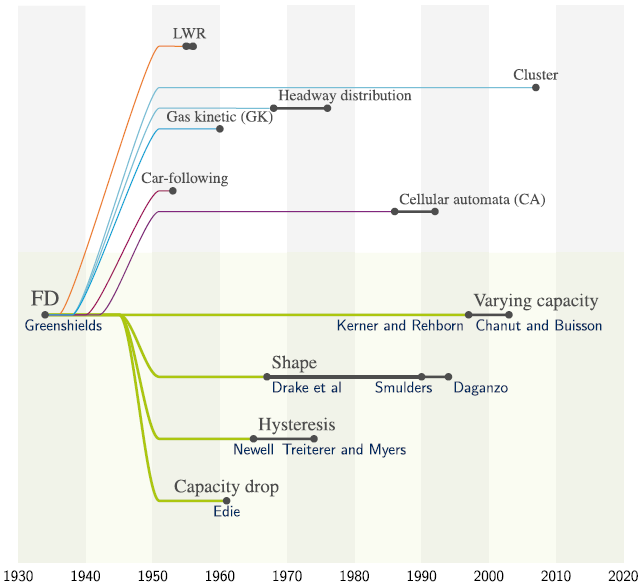
\includegraphics[width=0.9\textwidth]{family-tree}
 \caption[Überblick über die Entwicklung der Verkehrsflussmodelle]
 		{\enquote{Stammbaum} der Verkehrsflussmodelle, aus \cite{genealogy}}
 \label{figure:family-tree}
\end{figure}
\noindent
Die Fundamentalrelation, heute bekannt als Fundamentaldiagramm, kann aber auch mit Hilfe anderer Variablen, wie z. B. der Verkehrsdichte ($\rho$, der durchschnittlichen Anzahl von Fahrzeugen auf einer bestimmten Strecke) und dem Verkehrsfluss ($q$, der durchschnittlichen Anzahl von Fahrzeugen pro Zeiteinheit) wiedergegeben werden, siehe \cref{figure:fundamental-relations}. 
\begin{figure}[hptb]
 \centering
 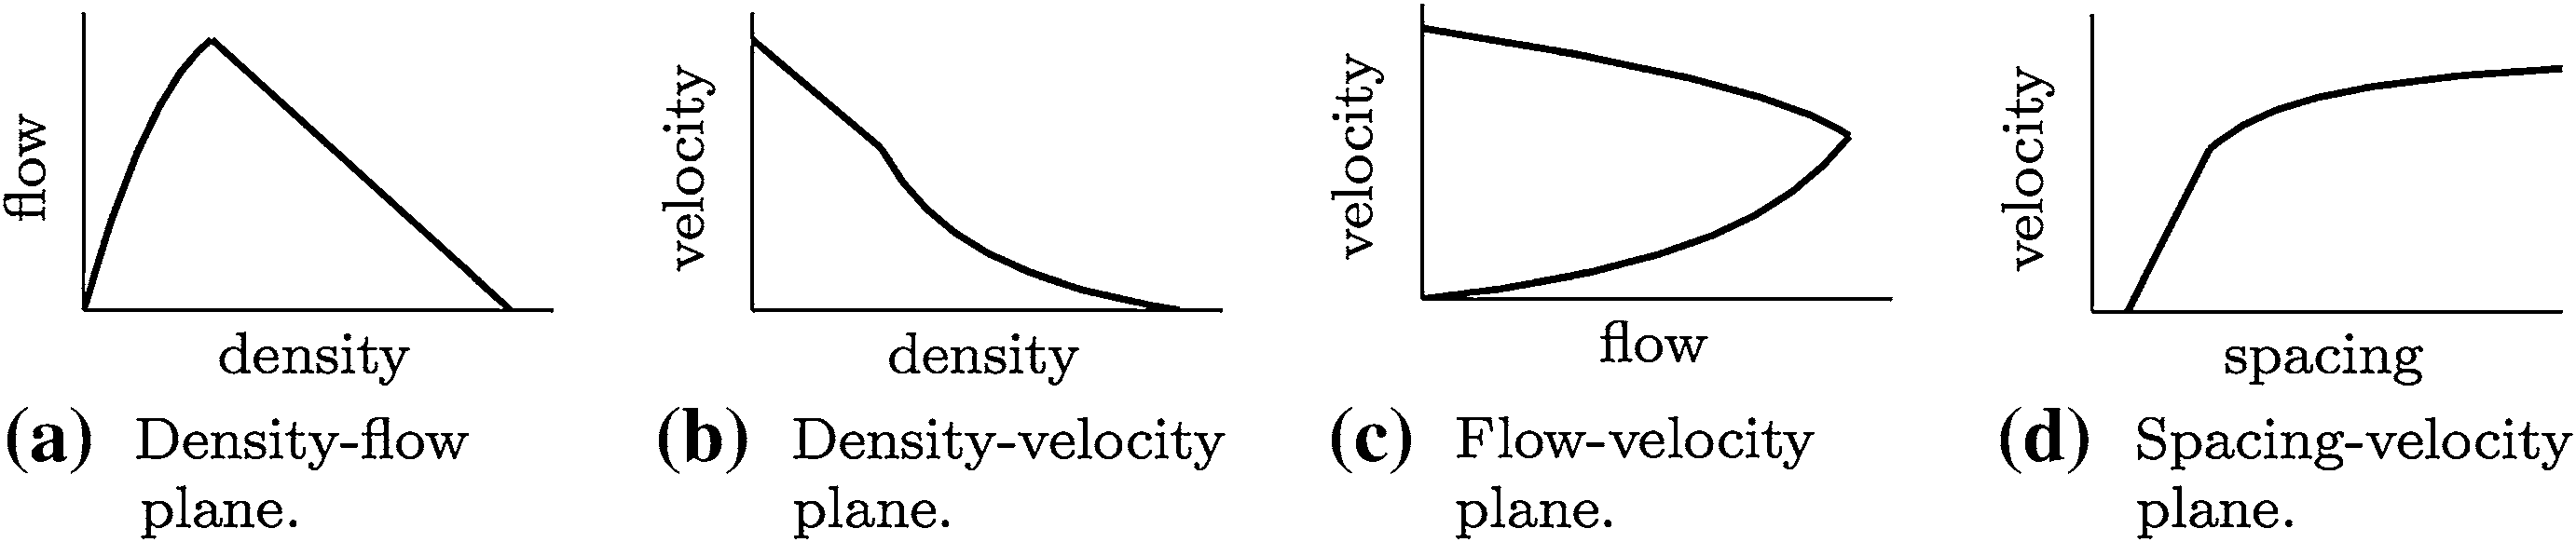
\includegraphics[width=0.9\textwidth]{fundamental-relations}
 \caption[Fundamentalrelationen in verschiedenen Ebenen]
 		{Fundamentalrelationen in verschiedenen Ebenen, aus \cite{genealogy}}
 \label{figure:fundamental-relations}
\end{figure}

Verschiedene Ansätze, Verkehrsflüsse zu simulieren, die auch unterschiedliche Sichtweisen auf Verkehr und Verkehrsteilnehmer verfolgen, %- mikro- makro- und mesoskopisch, 
wurden und werden verfolgt, vgl. \cite{dingding}.
\begin{itemize}
	\item \textit{Mikroskopische Modelle} simulieren einzelne Fahrzeug-Fahrer-Einheiten, basierend auf dem Fahrerverhalten. Zwei Modellierungsansätze können hier unterschieden werden: das Fahrzeugfolgemodell (\enquote{car-following model}) und das Zellularautomatenmodell. Zu letzterem später mehr.
	\item \textit{Makroskopische Modelle}  konzentrieren sich auf Charakteristiken des Verkehrsflusses, wie mittlere Geschwindigkeit (\enquote{average velocity}), Verkehrsdichte, -fluss und Durchschnittsgeschwindigkeit des Verkehrsstromes (\enquote{mean speed of a traffic stream}).
	\item \textit{Mesoskopische Modelle} kombinieren die beiden vorgenannten Modelle, simulieren die Fahrzeuge einzeln, nutzen aber die makroskopische Sicht, um deren Aktivitäten und Interaktionen zu beschreiben. Ein klassischer Vertreter ist das gaskinetische Modell.
\end{itemize}



\subsection{Zellularautomaten}
%\addcontentsline{toc}{subsection}{Zellularautomaten}
\label{sec:ca}

Zellularautomaten werden seit etwa 25-30 Jahren für die Verkehrssimulation verwendet.

\begin{quote}
Ein zellulärer Automat ist eine regelmäßige Annordnung von Zellen. Jede Zelle kann eine endliche Zahl von Werten / Zuständen annehmen und hat eine  begrenzte Zahl von Nachbarzellen, die sie beeinflussen können. Das Muster des gesamten zellulären Automaten ändert sich in einzelnen Schritten, die durch eine Reihe von Übergangsregeln bestimmt werden, die für alle Zellen gelten. (aus \cite{cell-autom})
\end{quote} 

\noindent
Vereinfacht kann eine Fahrspur einer Straße als Aneinanderreihung vieler Zellen gesehen werden(siehe \cref{figure:grid-umgebung}) und damit durch den Zellularautomaten abgebildet werden. 
\begin{figure}[hptb]
 \centering
 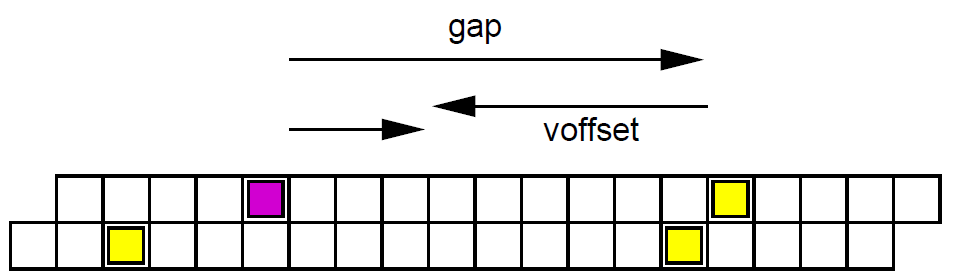
\includegraphics[width=0.9\textwidth]{grid-umgebung}
 \caption[Beispiel für eine Griddarstellung einer Straße]
 		{symbolische Griddarstellung einer Straße mit zwei Fahrspuren mit Fahrzeugen, aus \cite{multi-lane}}
 \label{figure:grid-umgebung}
\end{figure} \sa{einspurig croppen, obere Zeile und Richtungspfeil belassen}
Dies führt schließlich zu einer gridbasierten Simulationsumgebung. 


\subparagraph{Das Nagel-Schreckenberg-Modell}
%\subsubsection*{Das Nagel-Schreckenberg-Modell}
%\addcontentsline{toc}{subsubsection}{Das Nagel-Schreckenberg-Modell}
%\label{sec:na-sch}

Nagel und Schreckenberg war es 1992 gelungen, auf Basis solcher Automaten mit einfachen Regeln das mikroskopische Verhalten jedes Fahr\-zeug\-füh\-rers so abzubilden, dass sich die makroskopische Sicht auf den Verkehrsfluss als für Autobahnverkehr realistisch darstellte. 
Jedes Fahrzeug durchläuft in jedem Zeitschritt die folgenden Übergangsregeln, vgl. \cite{na-sch}. 

\begin{enumerate}
	\item \textit{Beschleunigung}: Solange ein Fahrzeug nicht seine max. Geschwindigkeit $v_{max}$ (Zellen/""Zeitschritt) erreicht hat und ein vorausfahrendes Fahrzeug weit genug entfernt ist, erhöht es die Geschwindigkeit um $1$, $v \rightarrow v+1$;
	\item \textit{Abbremsen}: Hat ein Fahrzeug ein anderes Fahrzeug $j$ Zellen vor sich, dann reduziert es die Geschwindigkeit auf $j-1$, $v \rightarrow j-1$;
	\item Zufallsgröße, auch \textit{\enquote*{Trödelwahrscheinlichkeit}}: Mit einer Wahrscheinlichkeit $p$ wird die Geschwindigkeit ($v > 0$) eines Fahrzeuges um $1$ reduziert, $v \rightarrow v-1$;
	\item \textit{Fahrzeugbewegung}: Jedes Fahrzeug wird um $v$ Zellen nach vorn gesetzt.
\end{enumerate}

\noindent
Erstmals konnte das Entstehen von \enquote{Stau aus dem Nichts} und das Vorhandensein von \enquote{Stauwellen}, die sich rückwärts durch einen solchen Stau bewegen, simulatorisch dargestellt werden.

Die Rechenumgebung wurde als eindimensionales Array mit $L$ Zellen definiert, $L$ ist dabei eine ganze Zahl. 
Jede der Zellen kann entweder von einem Fahrzeug belegt oder frei sein. 
Eine Simulation in dieser Grid-Welt hat den Vorteil, dass die Erkenntnisse auf die reale Welt skaliert werden können. 
Es wurde eine Zelllänge von 7,5\nolinebreak[4] m angenommen (vgl. \cite[S. 2227]{na-sch}), was ungefähr dem beanspruchten Platz eines Pkw - von Fahrzeugfront zu Fahrzeugfront - in einer Stausituation entspricht (Fahrzeuglänge + Abstand). 
Jedes Fahrzeug hat eine ganzzahlige Geschwindigkeit zwischen null und $v_{max}$.

\begin{table}[ht]
\begin{center}
\setlength{\tabcolsep}{0.5em} % for the horizontal padding
{\renewcommand{\arraystretch}{1.2}% for the vertical padding
\begin{tabular}{| c | c | c |}
\hline 
$v^{sim}$ in $\frac{\text{Zellen}}{\text{Zeitschritt}}$ & $\widehat{=}$ $v^{real}$ in $\frac{m}{s}$ & $=$ in $\frac{km}{h}$ \\ \hline 
$1$ & 7,5 & 27 \\ \hline
$2$ & 15 & 54 \\ \hline
$3$ & 22,5 & 81 \\ \hline
$4$ & 30 & 108 \\ \hline
$5$ & 37,5 & 135 \\ \hline
$6$ & 45 & 162 \\ \hline
\end{tabular}
}
\caption{Umrechnung Geschwindigkeiten Gridwelt $\rightarrow$ reale Welt}
\end{center}
\label{tab:umrechnung-zelle-kmh}
\end{table}

Zu Beginn eines Simulationslaufes wurden $N$ Fahrzeuge zufällig auf die $L$ Zellen verteilt.
Dies führte dazu, dass über den Durchlauf hinweg eine konstante Fahrzeugdichte $\rho$ im System garantiert werden konnte:
\begin{equation}
\rho = \dfrac{N}{L} = \dfrac{\text{Anzahl der Fahrzeuge im System}}{\text{Anzahl der Zellen des Systems}}
\nonumber
\end{equation}

\noindent
Die Simulation erfolgte unter Nutzung periodischer Randbedingungen. 
Wie in \cite[Abb. 1.5]{peri-rand} für die Umgebung von Pixeln beschrieben, werden die Fahrzeuge somit vom \enquote*{Ende} der Gridstrecke am \enquote*{Anfang} wieder eingesetzt. 
Damit einstand die Möglichkeit einer kontinuierlich arbeitenden Simulationsumgebung, siehe \cref{figure:traffic-simulation}.
\begin{figure}[hptb]
 \centering
 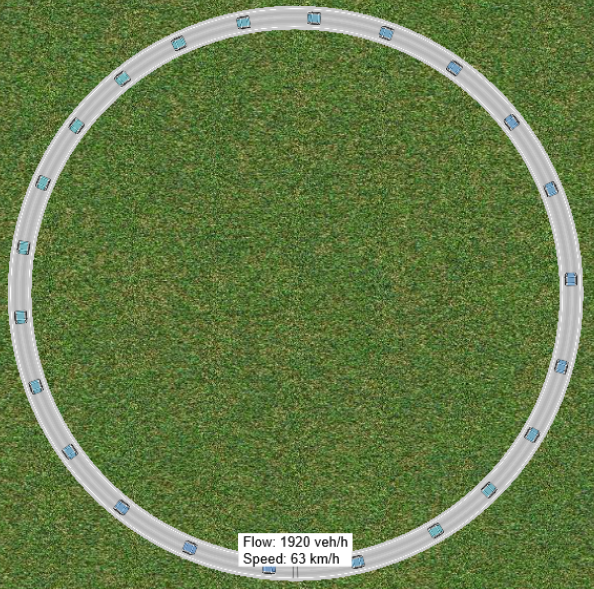
\includegraphics[width=0.75\textwidth]{traffic-simulation}
 \caption[Darstellung des Verkehrs in einem geschlossenen System]
 		{Symbolbild: Verkehr in einem Kreis (geschlossenes System), Screenshot \url{http://traffic-simulation.de}}
 \label{figure:traffic-simulation}
\end{figure} 



\subparagraph{Erweiterung auf Mehrspurigkeit}
%\subsubsection*{Erweiterung auf Mehrspurigkeit}
%\addcontentsline{toc}{subsubsection}{Erweiterung auf Mehrspurigkeit}
%\label{sec:multi-lane}

Um Verkehr auf mehrspurigen Fahrbahnen zu simulieren, war das Originalmodell nicht geeignet. 
1996 folgte deswegen eine Ausdehnung auf Mehrspurigkeit \cite{multi-lane} - zwei Spuren. 
Regeln, die prüfen, ob ein Spurwechsel vorteilhaft ist und einen sicheren, weil kollisionsfreien, und nicht behindernden Spurwechsel ermöglichen, wurden hinzugefügt. Die Regeln 1-3 wurden übernommen. Nach Simulationsläufen, die unerwünschtes Verhalten zeigten, waren die finalen Regeln wie folgt:

\textit{Hinweis:} $\Delta x$ $\widehat{=}$ dem Abstand zum vorausfahrenden Fahrzeug, die Indizes $b$ (\enquote*{behind} - für rückwärtigen Verkehr) und $o$ (\enquote*{other} - für Verkehr auf der Spur auf die gewechselt werden soll) können auch kombiniert werden. 

\begin{itemize}
	\item \textit{Sicherheitsbedingung}: die Geschwindigkeit des Fahrzeugs auf der Spur auf die gewechselt werden soll, darf nicht größer als der Abstand des Fahrzeugs sein (keine Behinderung des Nachfolgeverkehrs), $v^{o,b} \leq \Delta x^{o,b}-1$;
	\item \textit{Intention zum Spurwechsel}: Fahrzeug kann nicht so schnell fahren, wie es möchte, $v_{max} > \Delta x-1$ \\
	UND\\
	die andere Spur ist nicht schlechter als die aktuelle Spur, $\Delta x^{o} \geq \Delta x$
	\item \textit{nach dem Spurwechsel}: diese Regeln werden mit einer gewissen Wahrscheinlichkeit $p_{l2r}$ (\enquote{Zurückwechselwahrscheinlichkeit}) ausgeführt, \\
	ausreichend großer Abstand zum hinteren Fahrzeug auf der rechten Spur, $v^{o,b}_{max} \leq \Delta x^{o,b}-1$ \\
	UND \\
	ausreichend Platz auf der rechten Spur, $v \leq \Delta x^{o}-1$
\end{itemize}

Wenn es die festgelegten Kriterien zulassen, erfolgt der Spurwechsel auf die linke Spur immer, da dieser nicht an eine Wahrscheinlichkeit geknüpft ist.
Lediglich um die Überbevölkerung der Überholspur zu vermeiden, wurde eine Wahrscheinlichkeit $p_{l2r}$ für das zurückwechseln eingeführt.

Was dieser Modellierung fehlt, ist die Berücksichtigung irregulärer Verhaltensweisen der Fahrer - Unsicherheiten (z. B. Fehleinschätzungen oder Ängste), Ablenkungen (z. B. Gespräche mit anderen Fahrzeuginsassen, Telefonieren, Suche im Handschuhfach oder nach der fallen gelassenen Zigarette). 

Zusätzlich ist die Bremswirkung, wie auch im ursprünglichen Nagel-Schreckenberg-Modell, \enquote{über\-di\-men\-sio\-niert}. 
Vollbremsungen aus Höchstgeschwindigkeit sind innerhalb kürzester Distanz möglich \cite{acc-free}.
Daraus ergibt sich eine weitere fehlende Komponente der Realität.
Denn auch Unfälle gehören zum Verkehrsgeschehen. \\
Studien zufolge sind drei Viertel der Autofahrer abgelenkt, wenn sie am Steuer sitzen. 
Jeder zehnte Verkehrsunfall in Deutschland wird durch unaufmerksame Autofahrer verursacht. 
In Österreich und der Schweiz geht man, aufgrund der Einordnung in eine eigene Kategorie für diese Art Unfälle, von einer Rate von etwa 30\% der Unfälle mit Personenschäden oder gar Toten aus. (vgl. \cite{dvr-studie})

Laut Statistischem Bundesamt gab es 2016 auf Autobahnen 21193 Unfälle, davon 1435 innerhalb von Baustellen \cite{unf2016}. 
Bei den etwa 13000 km Autobahn \cite{autob2016} entspricht dies durchschnittlich etwa einem Unfall pro 200 km Strecke pro Tag. 
In Wirklichkeit wird es aber Unfallschwerpunkte geben, die diesen Durchschnittswert überschreiten.



\subsection{Stochastische Ansätze}
% \addcontentsline{toc}{subsection}{Stochastische Ansätze}
\label{sec:stochastic-approaches}

Es gibt inzwischen Ansätze, die das mikroskopische Verhalten der Fahrzeugführer aus Realdaten  stochastisch modelliert haben \cite{stoch-carfollow}. 
In den aggregierten Daten wurde eine Laplace-Verteilung der Beschleunigungswerte erkannt. 
Das daraus entwickelte Modell wurde getestet. 
Die Reproduktion der Sicherheitsparameter, wie Zeit bis zur Kollision (TTC, time to collision) und der Bremsrate um einen Unfall zu verhindern (DRAC, deceleration rate to avoid crash) gelang. 
Allerdings konnte das Fundamentaldiagramm nicht nachgestellt werden.

\cite{multi-fuzzy} integriert den Ansatz der Mehrspurigkeit in einem Multiagenten-Fuzzy-System. 
Die Spuren werden als Vereinigung mehrerer miteinander kommunizierender einspuriger Zellularautomaten (\enquote{continuous cellular automata}) beschrieben. 
Diese Kommunikation zwischen den Spuren beschränkt sich auf die Sicherheitskriterien, wenn ein Fahrzeug die Spur wechseln möchte. 
Intentionen zum Wechsel zwischen den Spuren werden durch fortwährend aktualisierte \enquote{Stresslevel} je Fahrzeug beeinflusst, die Wahrscheinlichkeiten dafür durch einen Bernoulli-Prozess berechnet.
Dieser Ansatz arbeitet mit Gridzellen und achtet auf Kollisionsfreiheit.



\subsection{Das Social-Force-Vehicle-Modell}
% \addcontentsline{toc}{subsection}{Das Social-Force-Vehicle-Modell}
\label{sec:social-force-vm}

In \cite{dat-ba} wurde mit dem \enquote{Social-Force-Vehicle-Modell} ein neuer Vorschlag für die Simulation von Spurwechseln entwickelt. 
Das Modell orientiert sich bei den Fahrzeugbewegungen an den Grundlagen des Nagel-Schreckenberg-Modells, vermeidet Unfälle aber in erster Linie nicht durch Abbremsen, sondern durch Ausweichen, also Spurwechsel. 

Im Gegensatz zur ursprünglichen erdachten Nutzung der \enquote{Social Forces} für Fußgänger, wie z. B. in \cite{soc-for} beschrieben, wird dieses System auf die Gridzellen angewandt, wirken als eine Art \enquote{Anziehungskraft} und liefern bei Auswahl einen Impuls für die Beibehaltung oder Änderung der Fahrspur. 
\begin{figure}[hptb]
 \centering
 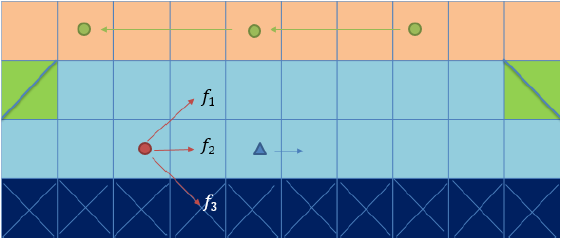
\includegraphics[width=0.7\textwidth]{social-forces}
 \caption[\enquote{Social Forces} für Grid-Zellen]{Vorschlag der \enquote{Social Forces} für Grid-Zellen (Fahrzeug auf Normalspur), aus \cite{dat-ba}}
 \label{figure:social-forces}
\end{figure}
\noindent
Von den ein Fahrzeug umgebenden acht Zellen müssen, aufgrund der Bewegungsrichtung, nur die drei betrachtet werden, die sich in Fahrtrichtung befinden.

Die Kräfte der Zellen, siehe \cref{figure:social-forces}, werden für jedes Fahrzeug zu jedem Zeitschritt $t$, da dessen Position zum Zeitpunkt $t + 1$ von der Position im vorhergehenden Zeitschritt abhängt, über verschiedene Funktionen berechnet. Das betrachtete Fahrzeug (Ego) befindet sich:
\begin{itemize}
	\item auf der Hauptspur 
	\begin{itemize}
		\item $f_{1}(a,v,\lambda) = \e^{\lambda(1-\frac{a}{v+\xi})}$ 
		\item $f_{2}(a,v,\lambda) = \frac{a}{\lambda(v+0,1)}$ 
		\item $f_{3} = 0$ 
	\end{itemize}
Hierbei ist $a$ der Abstand zum vorausfahrenden Fahrzeug, $v$ die relative Geschwindigkeit zwischen Ego und dem vorausfahrenden Fahrzeug und $\lambda$ ein Skalierungsfaktor. $\xi$ ist ein sehr kleiner positiver Wert, der die Durchführbarkeit der Division im Falle von $v=0$ sicherstellen soll. Für $f_{3}$ gibt es keinen Wert zu berechnen, da sich dort der Standstreifen befindet, der nicht befahren werden kann.
	\item auf der Überholspur 
	\begin{itemize}
		\item $h_{1} = 0$ 
		\item $h_{2}(a^{\prime},v^{\prime},\lambda) = \frac{v^{\prime}}{\lambda(a^{\prime}+0,1)}$ 
		\item $h_{3}(a^{\prime},v^{\prime},\lambda) = \e^{\lambda(1-\frac{v^{\prime}}{a^{\prime}+\omega})}$ 
	\end{itemize}
Hierbei ist $a^{\prime}$ der relative Abstand zum vorausfahrenden Fahrzeug auf der Hauptspur, $v^{\prime}$ die relative Geschwindigkeit zwischen Ego und dem vorausfahrenden Fahrzeug auf der Hauptspur und $\lambda$ auch hier der Skalierungsfaktor. $\omega$ entspricht $\xi$, im Fall dass $v^{\prime}=0$. Für $h_{1}$ wird kein Wert berechnet, da sich bei Betrachtung einer zweispurigen Fahrbahn in dieser Richtung keine weitere Spur in Fahrtrichtung befindet.
\end{itemize}

Die letztendliche Auswahl der Zielzelle für einen \enquote{Impuls zur Spurwahl} wird mittels \enquote{Fit\-ness-proportionate Selection} durchgeführt.

%%%%%

\subparagraph{\enquote{Fitness-proportionate Selection} oder \enquote{Roulette-wheel sampling}}

Die Konzept der \enquote{Fitness-proportionate Selection} kommt aus dem Bereich der genetischen Algorithmen. 
\cite{gen-algo} beschreibt es in einem Beispiel anhand einer Population von $n=4$ Strings, die man repräsentativ auch als Individuen oder Wahlmöglichkeiten ansehen kann. 
Jedem dieser Strings ist ein Funktionswert $f$ (Fitnesswert), ein Maß für Profit, Nutzwert oder Güte zugeordnet, den es zu maximieren gilt. 
Strings mit einem höheren Fitnesswert haben eine höhere Wahrscheinlichkeit, einen oder mehrere Nachkommen für die Folgegeneration beizutragen.
Demnach ist dies eine künstliche Version des Darwin'schen \enquote{Survival of the Fittest}.

\begin{table}[ht]
\begin{center}
\setlength{\tabcolsep}{0.5em} % for the horizontal padding
{\renewcommand{\arraystretch}{1.2}% for the vertical padding
\begin{tabular}{| l  c  c |}
\hline 
No. & Fitnesswert $f$ & \% von Gesamt \\ \hline 
1 & 169 & 14,4 \\ 
2 & 576 & 49,2 \\ 
3 & 64 & 5,5 \\ 
4 & 361 & 30,9 \\ \hline
Gesamt & 1170 & 100,0 \\ \hline
\end{tabular}
}
\caption{Beispiel nach \cite[Table 1.1]{gen-algo}}
\label{tab:beispiel-tabelle-roulette}
\end{center}
\end{table}

Ein einfacher Weg \textit{Fitness-proportionate Selection} zu veranschaulichen ist \textit{Roulette-wheel sampling}. 
Dabei wird jeder Option ein Bereich (Slot) auf einem Rouletterad zugewiesen, welcher von der Größe her deren Fitnesswert entspricht, siehe \cref{figure:meta-chart}. 

\begin{figure}[hptb]
 \centering
 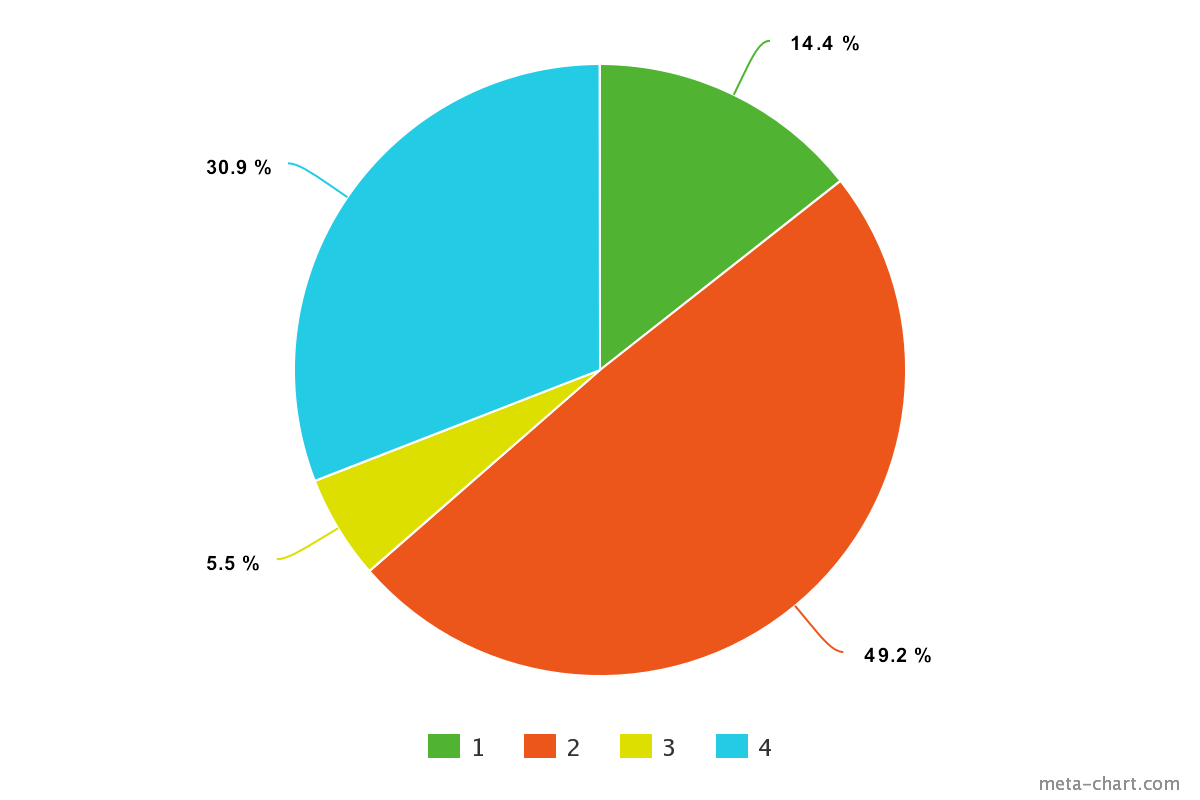
\includegraphics[width=0.7\textwidth]{meta-chart}
 \caption[gewichtetes Roulette-Rad (fitness-proportionate selection]
 		{schematische Darstellung eines gewichteten Rouletterades für der Beispiel in \cref{tab:beispiel-tabelle-roulette}}
 \label{figure:meta-chart}
\end{figure}

Benötigt man z. B. auch in der Nachfolgegeneration vier Strings, würde das Rouletterad viermal gedreht.
Das Individuum in dessen Slot die Kugel liegen bleibt, würde ausgewählt.

Aufgrund der Größe der Slots von String 2 und String 4 ist es z. B. möglich, dass String 2 für die Kindgeneration zweimal und String 4 gar nicht ausgewählt wird.

%%%%%

\subparagraph{Verwendung im Social-Force-Vehicle-Modell}

Im Social-Force-Vehicle-Modell gibt es zwei Möglichkeiten, aus denen gewählt werden kann. 
Zum einen jeweils das Geradeausfahren, zum anderen die Möglichkeit aus- respektive einzuscheren.
Für die Wahl der Alternative ist nur eine Entscheidung zwischen den jeweils zwei Möglichkeiten nötig.

Entgegen des Zwangs zum Ausscheren oder einer vorgegebenen Wahrscheinlichkeit für das Einscheren in der mehrspurigen Version des Nagel-Schreckenberg-Modells wird eine stochastische Simulationsmöglichkeit der Neigung zum Spurwechsel aufgezeigt.
Es entsteht eine Ungewissheit, ob die wahrscheinlichste Alternative ausgewählt wird oder ob die andere, weniger wahrscheinliche, das Verhalten bestimmen wird. 

\subparagraph{Möglichkeit von Kollisionen im Social-Force-Vehicle-Modell}

Da Kollisionen im Modell durch Ausweichen verhindert werden sollen, aber die \enquote{Bremskomponente} aus dem Ursprungsmodell entfernt wurde, ist in bestimmten Situationen ein Auffahrunfall denkbar.



%Bereits seit den 1950er Jahren wurden strömungsdynamische Ansätze für die Simulation von Verkehrsflüssen entwickelt. 
%Außerdem gab es ab den 1980er Jahren auch boolsche Simulationsmodelle, die mit Gitter-Gas-Automaten Flüssigkeiten simulieren konnten.
%Anfang der 1990er wurde von Kai Nagel und Michael Schreckenberg in \cite{na-sch} ein Verfahren vorgestellt, welches Autobahnverkehr basierend auf Zellularautomaten modelliert. 
%
%\begin{quote}
%Ein zellulärer Automat ist eine regelmäßige Annordnung von Zellen. Jede Zelle kann eine endliche Zahl von Werten / Zuständen annehmen und hat eine  begrenzte Zahl von Nachbarzellen, die sie beeinflussen können. Das Muster des gesamten zellulären Automaten ändert sich in einzelnen Schritten, die durch eine Reihe von Übergangsregeln bestimmt werden, die für alle Zellen gelten. (aus \cite{cell-autom})
%\end{quote}
%
%\noindent
%Vereinfacht kann eine Fahrspur einer Straße als Aneinanderreihung vieler solcher Zellen gesehen werden. 
%Dies führt schließlich zu einer gridbasierten Simulationsumgebung. 
%In \cite{na-sch} wird die Rechenumgebung als eindimensionales Array mit $L$ Zellen definiert. 
%Jede der Zellen kann entweder von einem Fahrzeug belegt oder frei sein. 
%Eine Simulation in dieser Grid-Welt hat den Vorteil, dass die Erkenntnisse auf die reale Welt skaliert werden können. 
%Es wird eine Zelllänge von 7,5\nolinebreak[4] m angenommen (vgl. \cite[S. 2227]{na-sch}), was ungefähr dem beanspruchten Platz eines Pkw - von Fahrzeugfront zu Fahrzeugfront - in einer Stausituation entspricht (Fahrzeuglänge + Abstand). 
%Jedes Fahrzeug hat eine ganzzahlige Geschwindigkeit zwischen null und $v_{max}$.
%
%\begin{table}[ht]
%\begin{center}
%\setlength{\tabcolsep}{0.5em} % for the horizontal padding
%{\renewcommand{\arraystretch}{1.2}% for the vertical padding
%\begin{tabular}{| c | c | c |}
%\hline 
%$v^{sim}$ in $\frac{Zellen}{Zeitschritt}$ & $\widehat{=}$ $v^{real}$ in $\frac{m}{s}$ & $=$ in $\frac{km}{h}$ \\ \hline 
%$1$ & 7,5 & 27 \\ \hline
%$2$ & 15 & 54 \\ \hline
%$3$ & 22,5 & 81 \\ \hline
%$4$ & 30 & 108 \\ \hline
%$5$ & 37,5 & 135 \\ \hline
%$6$ & 45 & 162 \\ \hline
%\end{tabular}
%}
%\caption{Umrechnung Geschwindigkeiten Gridwelt $\rightarrow$ reale Welt}
%\end{center}
%\label{tab:umrechnung-zelle-kmh}
%\end{table}
%
%\noindent
%Die beobachtete Durchschittsgeschwindigkeit von 4,5 Zellen/Zeitschritt, der als eine Sekunde angenommen wird, entspricht etwa der einer Geschwindigkeit von 120 km/h (vgl. \cite[S. 2227]{na-sch}). 
%
%In \cite{na-sch} war es erstmals gelungen, Wechselwirkungen zwischen Fahrzeugen im Einspurfall darzustellen und u. a. das Entstehen von Staus, ohne dass ein Grund dafür vorlag, zu modellieren. 
%Mit drei Regeln, die auf jedes Fahrzeug gleichzeitig und gleichermaßen anzuwenden waren, wurde ein realistischer Verkehrsfluss generiert. 
%Die folgenden Regeln, die die Kollisionsfreiheit sichern, sind die Grundlage für die, heute als \enquote{Nagel-Schreckenberg-Modell} bekannte, Modellierung:
%
%\begin{itemize}
%\item \textit{Beschleunigung}: Solange ein Fahrzeug nicht seine max. Geschwindigkeit $v_{max}$ (Zellen/""Zeitschritt) erreicht hat und ein vorausfahrendes Fahrzeug weit genug entfernt ist, erhöht es die Geschwindigkeit um $1$, $v \rightarrow v+1$;
%\item \textit{Abbremsen}: Hat ein Fahrzeug ein anderes Fahrzeug $j$ Zellen vor sich, dann reduziert es die Geschwindigkeit auf $j-1$, $v \rightarrow j-1$;
%\item Zufallsgröße, auch \textit{\enquote*{Trödelwahrscheinlichkeit}}: Mit einer Wahrscheinlichkeit $p$ wird die Geschwindigkeit ($v > 0$) eines Fahrzeuges um $1$ reduziert, $v \rightarrow v-1$
%\end{itemize}
%
%\noindent
%Die Anweisungen werden in der angegebenen Reihenfolge - für alle Fahrzeuge gleichzeitig - ausgeführt und jedes Fahrzeug um die entsprechende Anzahl Zellen weiter gesetzt.
%
%Dehnt man dieses Modell aber auf mehrere Fahrspuren aus, stößt es an seine Grenzen, weil die Modellierung von Überholvorgängen, bzw. genauer gesagt für das \enquote{Ausscheren} und \enquote{Einscheren}, nicht Teil des ursprünglichen Modells ist. 
%\cite{multi-lane} liefert eine \enquote*{multi-lane}-Betrachtung, wobei die ursprünglichen drei Regeln durch weitere ergänzt wurden, die zum einen ein Auffahren des Nachfolgeverkehrs auf den Spurwechsler und zum anderen auch des die Spur wechselnden auf vorausfahrende Fahrzeuge verhindern. \\
%In der Betrachtung, ob die Aktualisierung der Fahrzeuge parallel oder sequentiell erfolgen soll, wurde erkannt, dass dies für das entwickelte Modell nur geringe Unterschiede macht, da die Rate der Spurwechsel mit den festgelegten Regeln eher gering ist. \\
%Gleichzeitig wurde auch beobachtet, dass Fahrzeuge nicht wieder von der Überholspur in die Normalspur wechselten. Dies wurde mit weiteren Regeln und einer Spurwechselwahrscheinlichkeit abgestellt. Eine weitere Kalibrierung des Modells wurde in einer Folgearbeit durchgeführt. \\
%Durch die Konstanthaltung der Anzahl generierter Fahrzeuge und die Veränderung der Systemgröße konnten verschiedene Verkehrsdichten simuliert werden.
%
%\cite{multi-lane} zeigt mehrere Diagramme. Eine Untersuchung von realen Spurwechselvorgängen ergab, dass eine Umkehr der Benutzungshäufigkeit der rechten und linken Spuren bei einem Verkehrsfluss $q_{12}$ von etwa 1200 (Fahrzeugen) pro Stunde auf beiden Spuren erfolgt.
%
%Die Simulation ergab, dass der Punkt, an dem beide Spuren gleichermaßen benutzt werden, deutlich unter dem Punkt liegt, an dem der maximale Verkehrsfluss erreicht wird, siehe \cref{figure:verkehrsfluss-spurnutzung}.
%
%\begin{figure}[hptb]
% \centering
% 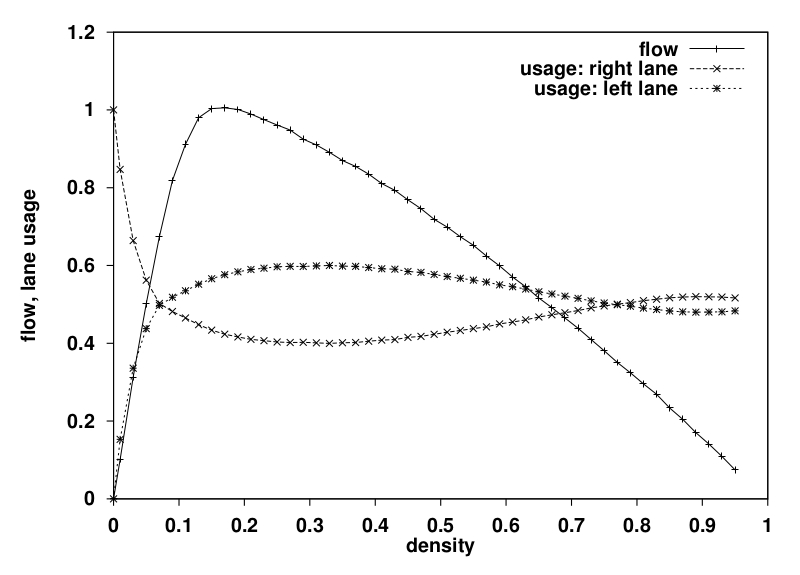
\includegraphics[width=0.7\textwidth]{verkehrsfluss-spurnutzung}
% \caption[Verkehrsfluss und Spurnutzung als Funktion der Verkehrsdichte]{Verkehrsfluss und Spurnutzung als Funktion der Verkehrsdichte, aus \cite{multi-lane}}
% \label{figure:verkehrsfluss-spurnutzung}
%\end{figure}
%
%\noindent
%Ein weiteres Resultat der Simulation ist eine mehrfache Umkehr der Nutzung der Fahrspuren abhängig von der Verkehrsdichte, wenn andere Parameter konstant gehalten werden, siehe \cref{figure:verkehrsfluss}.
%
%\begin{figure}[hptb]
% \centering
% 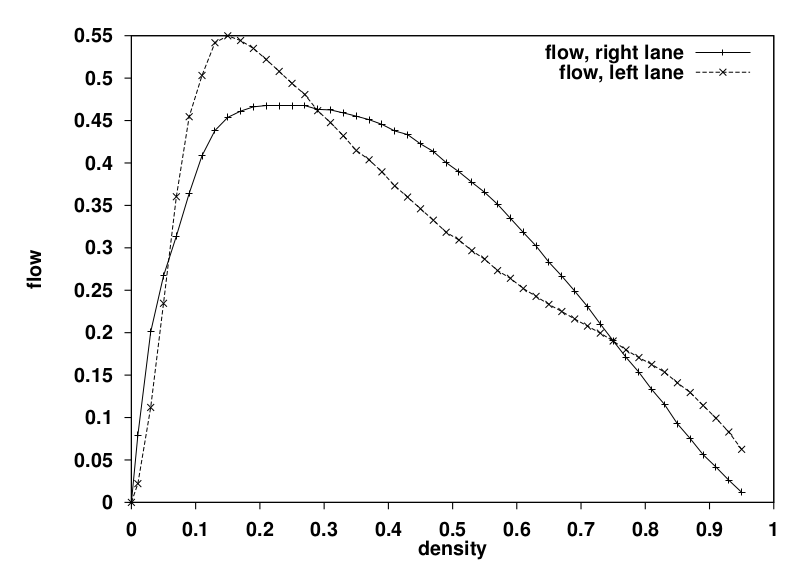
\includegraphics[width=0.7\textwidth]{verkehrsfluss}
% \caption[Verkehrsfluss als Funktion der durchschnittlichen Verkehrsdichte]{Verkehrsfluss auf den Fahrspuren als Funktion der durchschnittlichen Verkehrsdichte, aus \cite{multi-lane}}
% \label{figure:verkehrsfluss}
%\end{figure}
%
%\noindent
%Die Festlegung einer Wahrscheinlichkeit für das Zurückwechseln von der linken auf die rechte Fahrspur führte zu einer unterschiedlichen Spurwechselfrequenz, siehe \cref{figure:spurwechselfrequenz}.
%
%\begin{figure}[hptb]
% \centering
% 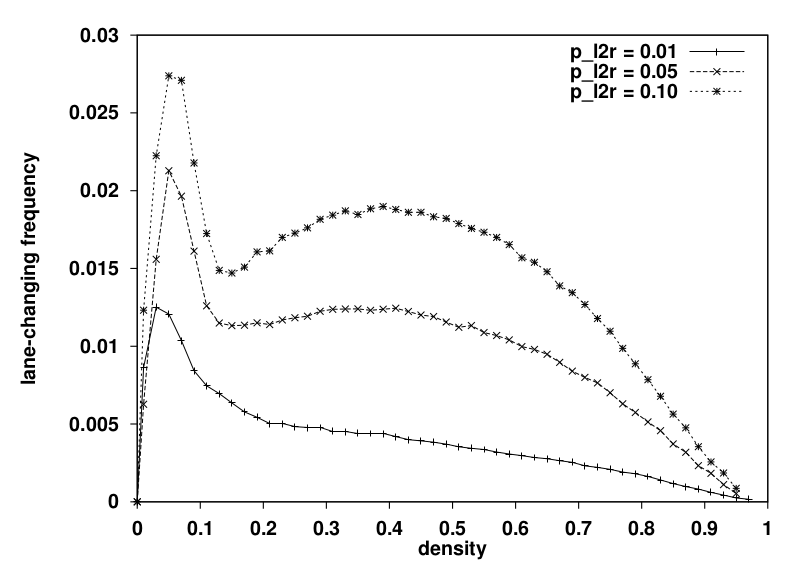
\includegraphics[width=0.7\textwidth]{spurwechselfrequenz}
% \caption[Spurwechselfrequenz als Funktion der Verkehrsdichte]{Spurwechselfrequenz als Funktion der Verkehrsdichte für verschiedene Spurwechselwahrscheinlichkeiten, aus \cite{multi-lane}}
% \label{figure:spurwechselfrequenz}
%\end{figure}
%
%\pagebreak
%In \cite{dat-ba} wurde mit dem \enquote{Social-Force-Vehicle-Modell} ein neuer Ansatz für die Simulation von Spurwechseln entwickelt.
%Auch hier wird eine Grid-Umgebung verwendet.
%Im Gegensatz zur ursprünglichen erdachten Nutzung der \enquote{Social Forces} für Fußgänger, wie z. B. in \cite{soc-for} beschrieben, wird dieses System auf die Gridzellen angewandt. Die Kräfte der Zellen, siehe \cref{figure:social-forces}, werden für jedes Fahrzeug zu jedem Zeitschritt $t$ berechnet, da seine Position zum Zeitpunkt $t + 1$ von der Position im vorhergehenden Zeitschritt abhängt.
%Von den ein Fahrzeug umgebenden acht Zellen müssen, aufgrund der Bewegungsrichtung, nur die drei betrachtet werden, die sich in Fahrtrichtung befinden.
%
%\begin{figure}[hptb]
% \centering
% 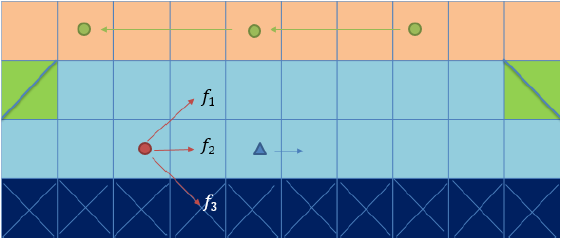
\includegraphics[width=0.7\textwidth]{social-forces}
% \caption[\enquote{Social Forces} für Grid-Zellen]{Vorschlag der \enquote{Social Forces} für Grid-Zellen, aus \cite{dat-ba}}
% \label{figure:social-forces}
%\end{figure}
%
%\noindent
%Die letztendliche Auswahl der Zielzelle wird mittels \enquote{Fitness-proportionate Selection} durchgeführt.
%Entgegen des Zwangs zum Ausscheren und einer fest vorgegebenen Wahrscheinlichkeit wird eine stochastische Simulationsmöglichkeit der Neigung zum Spurwechsel aufgezeigt. 
    \section{Research Gap}
\label{sec:researchgap}

In der Multi-Lane-Version des Nagel-Schreckenberg-Modells (siehe \cite{multi-lane}) geben die Regeln einen Zwang zum Einleiten des Überholvorganges, wenn sich die Möglichkeit dazu ergibt, vor. Ebenso wurde für den Rückwechsel auf die Normalspur eine Wahrscheinlichkeit festgelegt.

Das Verhalten des Entscheiders Mensch, was auch im Straßenverkehr eine große Rolle spielt, wurde bisher eher als eine Art \enquote{Black Box} betrachtet. 
Jeder Fahrzeugführer trifft zu jedem Zeitpunkt unter gleichen Voraussetzungen die gleiche Entscheidung. 
Dies ist aber in der Realität nicht so. 
Ein Fahrer kann z. B. vorsichtiger sein als ein anderer und, trotz des gleichen Abstands und der gleichen Geschwindigkeiten, auf ein Überholmanöver verzichten, weil er seine Umwelt anders einschätzt.

In \cite{dat-ba} wird der Hang zum Wechsel oder zur Beibehaltung der Spur nicht nur durch fest vorgegebene Wahrscheinlichkeiten simuliert, sondern durch individuell für jedes Fahrzeug zu jedem Zeitschritt berechnete \enquote{Kräfte}, deren \enquote*{Entscheidung}, durch entsprechende berechnete Wahrscheinlichkeiten getragen, mehr oder weniger häufig zur Ausführung kommen. 
Durch die gezielte Beachtung des umgebenden Verkehrs und das Bewerten der zur Wahl stehenden Alternativen soll es nun möglich sein, das menschliche Verhalten besser als bisher abzubilden.

Das Hauptaugenmerk von \cite{dat-ba} lag auf der theoretischen Modellentwicklung/""Modellierung. 
Eine praktische Umsetzung und somit die Kontrolle des Erdachten und natürlich die Möglichkeit eines Vergleichs zwischen dem neuen Ansatz und bereits existierenden Modellierungen, z. B. dem Mehrspurmodell aus \cite{multi-lane}, ist bisher nicht durchgeführt worden. 
Dies ist Ziel dieser Arbeit.

\subsection*{Mögliches Problem}
\addcontentsline{toc}{subsection}{Mögliches Problem}

Aus der Art und Weise, wie der Ansatz in das ursprüngliche Modell nach \cite{na-sch} (und nicht in die Mehrspurvariante nach \cite{multi-lane}) integriert wurde, könnte ein Problem entstehen.
Eine der drei Regeln, die die Kollisionsfreiheit sichern sollen - das Abbremsen - wurde entfernt und durch das \enquote{Social-Force-Modell} ersetzt (siehe \cite{dat-ba}, S. 21 \& Abb. 16, bzw. Vortragsfolien S. 7).
Dies kann dazu führen, dass in der Simulation ein Auffahrunfall unausweichlich ist.
Auch wenn Verkehrsunfälle in der realen Welt durchaus vorkommen, sollte man sie in dieser Simulation nicht provozieren. Zudem ist die Unfallhäufigkeit so gering, dass sie bei betrachteter Zeitspanne und Streckenlänge unbedeutend ist.

\begin{figure}[hptb]
 \centering
 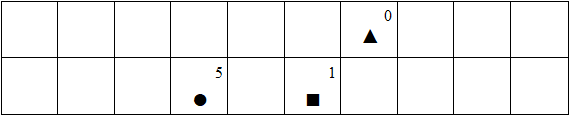
\includegraphics[width=0.6\textwidth]{problem-beispiel}
 \caption[Problem-Beispiel]{Beispiel für ein Problem-Szenario, drei Fahrzeuge und deren Geschwindigkeiten}
 \label{figure:problem-beispiel}
\end{figure}

\noindent
In \cref{figure:problem-beispiel} würde dem Fahrzeug $\bullet$ nach dem Multi-Lane-Modell aus \cite{multi-lane} das Ausscheren vorgegeben, denn die linke Spur bietet mehr Platz als die rechte und es gibt keinen nachfolgenden Verkehr auf der anderen Spur. 
Fahrzeug $\blacktriangle$ ist $j=3$ Felder vor $\bullet$.
Ein Abbremsen von $\bullet$ auf $v_{\bullet}=j-1=2$ würde veranlasst.
Dass $\blacktriangle$ gleichzeitig um $1$ beschleunigen könnte, spielt keine Rolle. \\
Nach dem \enquote{Social-Force-Modell} würde für das Fahrzeug $\bullet$ wahrscheinlich eine höhere Kraft der entsprechenden Zelle und somit Wahrscheinlichkeit für das Ausscheren berechnet werden.
Dies muss aber nicht zur Entscheidung in Richtung Spurwechsel führen.
$\blacksquare$ kann im aktuellen Zeitschritt max. auf $v_{\blacksquare}=2$ beschleunigen, $\blacktriangle$ max. auf $v_{\blacktriangle}=1$.
Da Fahrzeug $\bullet$ seine Geschwindigkeit aber nur durch die Zufallsgröße \enquote{Trödeln} um max. $1$ reduzieren könnte, würde es beim Simulationsschritt \enquote{Fahren} auf das gleiche Grid-Feld oder gar davor gesetzt werden. \\
Da ein solches Szenario insbesondere bei Stockungen und an Stauenden auftreten dürfte, wären dort Auffahrunfälle unvermeidbar. 

Das \enquote{Social-Force-Modell} wird im normalen Verkehrsfluss einen Teil der möglichen Unfallszenarien durch Ausweichen verhindern, aber bei \enquote*{Auswahl} der weniger wahrscheinlichen Alternative geradeaus zu fahren, wird sich das fehlende \enquote*{Bremsen} bemerkbar machen.

    \section{Realisierung}
\label{sec:realisierung}

Das Simulationstool, welches für diese Arbeit verwendet wurde, ist eine Modifikation einer Software, die als \enquote{Traffic Simulation Game} für einen Workshop für Doktoranden\footnote{\url{https://lightjason.github.io/news/2017-09-workshop/}} erstellt wurde.

In diesem Workshop mussten die Teilnehmer mit Hilfe der Agentensprache ein Fahrzeug so steuern, dass dieses auf einem 50 km langen Straßenstück, welches zufällig Bereiche mit unterschiedlich hohen Geschwindigkeitsbegrenzungen enthielt, möglichst wenige Verkehrsverstöße beging und die Strecke dennoch möglichst schnell zurücklegt.

Für die Zwecke dieser Arbeit musste die Software angepasst werden.
Dabei mussten während der Tests der ersten Agentenpläne Korrekturen vorgenommen werden, da sonst eine fehlerfreie Simulation nicht möglich gewesen wäre. 
Mehr dazu nachfolgend in \cref{sec:anpassungen-probleme}.
\pk{Kann, darf, soll, muss ich hier darauf hinweisen, dass die Programmierung nicht meine Aufgabe war und dass Du das gemacht hast?}
\sa{Das musst Du sogar machen, das war aber eine explizite Vorgabe für Deine Arbeit, Du solltest aber auch dazu schreiben, dass Du eben einige Anpassungen gemacht hast, da es nicht richtig funktioniert hat}




\subsection{Anpassungen der Simulationssoftware}
\label{sec:anpassungen-probleme}

Einer der Hauptunterschiede zur Softwareversion des Workshops ist, dass die Simulationen hier auf einer unendlichen Strecke stattfinden.
Fahrzeuge, die das Streckenende passieren, werden mit gleichen Verhaltenswerten am Anfang wieder eingesetzt.
Dieses Umsetzen selbst bereitete keine Probleme, allerdings resultierten solche aus der Unterbrechung der Strecke.



\subsubsection{Schwierigkeiten bei der Simulation der Ringform der Strecke}
\label{sec:probleme-ringform}

Die Streckenunterbrechung führte dazu, dass es eine Pause in der Sichtbarkeit der Fahrzeuge untereinander gab, wenn sich diese an unterschiedlichen Enden der Strecke befanden.
Aufgrund dieser \enquote{Unsichtbarkeit} war es unmöglich, eine Abstandsberechnung zwischen den einzelnen Fahrzeugen durchzuführen und führte zu einer freien Beschleunigung, da eine freie Strecke vermutet wurde.

Nachfolgend ist dies anhand eines Auszugs aus einem Log einer Simulation mit zwei Fahrzeugen dargestellt.
\enquote{...} bezeichnet Kürzungen der Ausgabe.

In Zeitschritt 315 war Fahrzeug \texttt{vehicle20} gerade noch in der letzten Zelle der Fahrbahn und überschreitet diese Grenze einen Zeitschritt später.
Die Beliefliste beider Fahrzeuge ist ab dem Schritt 316 leer.
Erst nach vier Zeitschritten befindet sich auch das Folgefahrzeug (\texttt{vehicle0}) am Anfang der Fahrspur und ist ab Zeitschritt 320 wieder für Fahrzeug \texttt{20} sichtbar (andersherum ebenso).

\footnotesize\begin{verbatim}
----- step 315 ----------------
      vehicle0   -> BELIEFLIST   [view/vehicle[id[vehicle20], ... direction[forward[]]]]]]
      vehicle20   -> BELIEFLIST   [view/vehicle[id[vehicle0], ... direction[backward[]]]]]]
      vehicle0   in lane   1   in cell   331.0   @   87.11188616490347   kph
      vehicle20   in lane   1   in cell   400.0   @   88.65039571533352   kph
----- step 316 ----------------
      vehicle0   -> BELIEFLIST   []
      vehicle20   -> BELIEFLIST   []
      vehicle0   in lane   1   in cell   345.0   @   87.89778423377561   kph
      vehicle20   in lane   1   in cell   14.0   @   88.65039571533352   kph
----- step 317 ----------------
...
----- step 318 ----------------
...
----- step 319 ----------------
      vehicle0   -> BELIEFLIST   []
      vehicle20   -> BELIEFLIST   []
      vehicle0   in lane   1   in cell   387.0   @   89.01152857206483   kph
      vehicle20   in lane   1   in cell   56.0   @   88.65039571533352   kph
----- step 320 ----------------
      vehicle0   -> BELIEFLIST   [view/vehicle[id[vehicle20], ... direction[forward[]]]]]]
      vehicle20   -> BELIEFLIST   [view/vehicle[id[vehicle0], ... direction[backward[]]]]]]
      vehicle0   in lane   1   in cell   1.0   @   89.79742664093698   kph
      vehicle20   in lane 1 in cell 70.0 @ 88.65039571533352 kph
\end{verbatim}
\normalsize

Für die Simulation mit mehreren Fahrzeugen stellte dies insbesondere ein Problem dar, weil eine Stauwelle, die sich in ihrer Rückwärtsbewegung dem Anfang der Strecke näherte, von Fahrzeugen am Ende der Strecke nicht erkannt werden konnte.
Dies führte zu dem Verhalten, dass Fahrzeuge vom Ende der Strecke an den Anfang gesetzt werden sollten, dort aber nicht in eine freie Zelle gesetzt werden konnten.
Die Simulationsumgebung sieht hier vor, dass das Fahrzeug auf die freie Zelle hinter das jeweils letzte Fahrzeug gesetzt wird.
\\
Zelle 1 ist die erste zu besetzende Zelle einer Lane, die freie Zelle hinter dem Fahrzeug war Zelle 0.
Allerdings wurden die Fahrzeuge, die sich bereits dort befanden, jeweils noch ein Feld weiter nach hinten gesetzt und das neue Fahrzeug dazwischen einfügt.

Es ergab sich bei einigen Simulationsläufen ein Häufung von Positionspunkten im negativen Teil der Strecke.
In der Simulation in \cref{figure:negativ-sammeln} trat das Problem direkt am Anfang des Durchlaufs aufgrund der langen Standzeit (siehe \cref{sec:accelerategroove}) des direkt am Anfang der Lane verorteten Fahrzeuges auf und konnte über die Simulationsdauer nicht abgebaut werden.
\begin{figure}[hptb]
 \centering
 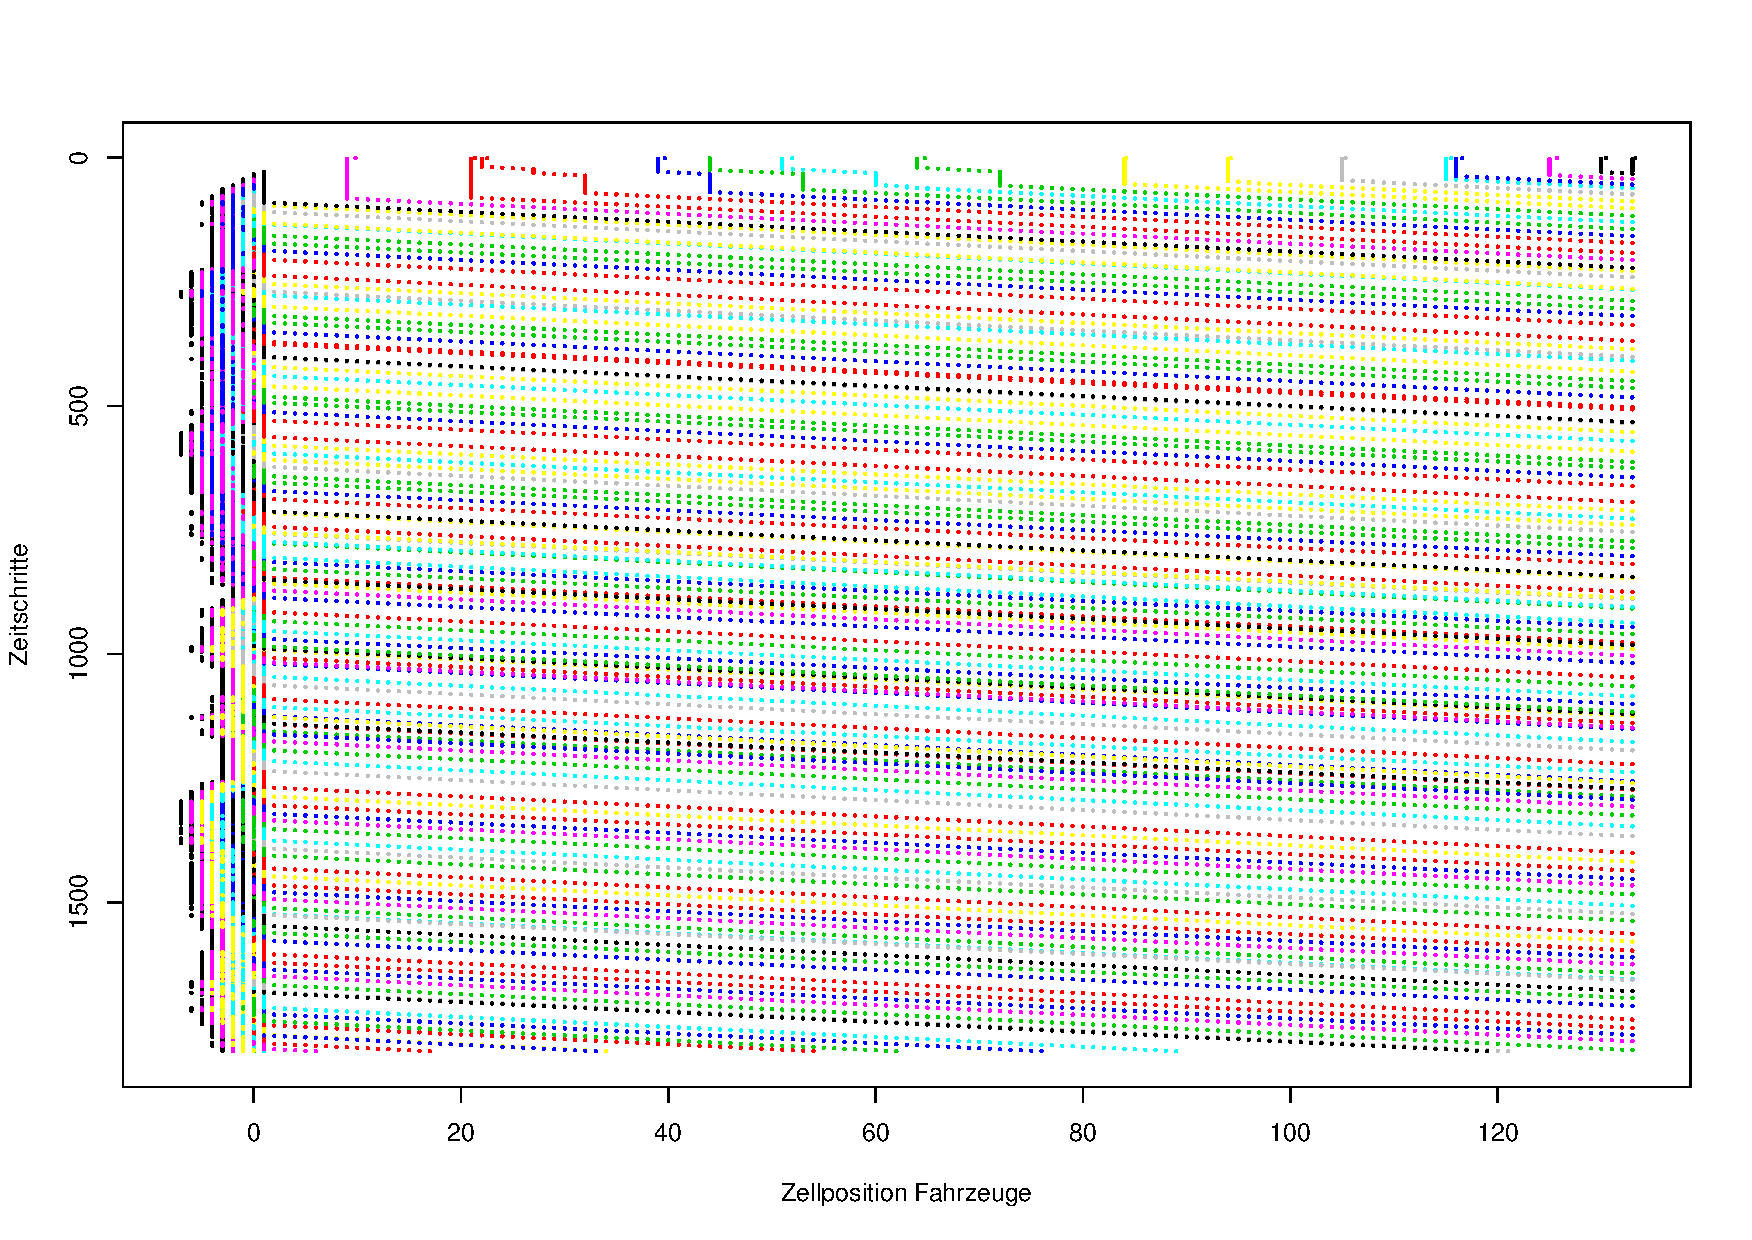
\includegraphics[width=0.9\textwidth]{negativ-sammeln}
 \caption[Punktehäufung im negativen Bereich]
 		 {Häufung der Punkte im negativen Bereich (Position-Zeit-Diagramm)}
 \label{figure:negativ-sammeln}
\end{figure} 

In \cref{figure:view-range-no-clip} wird die Problematik beispielhaft am Sichtfeld des gelben Fahrzeugs grafisch verdeutlicht. 
Gleiches gilt analog für die rückwärtige Sicht des violetten Fahrzeugs.

\begin{figure}[hptb]
  \centering
    \subfigure[ohne Umbruch]{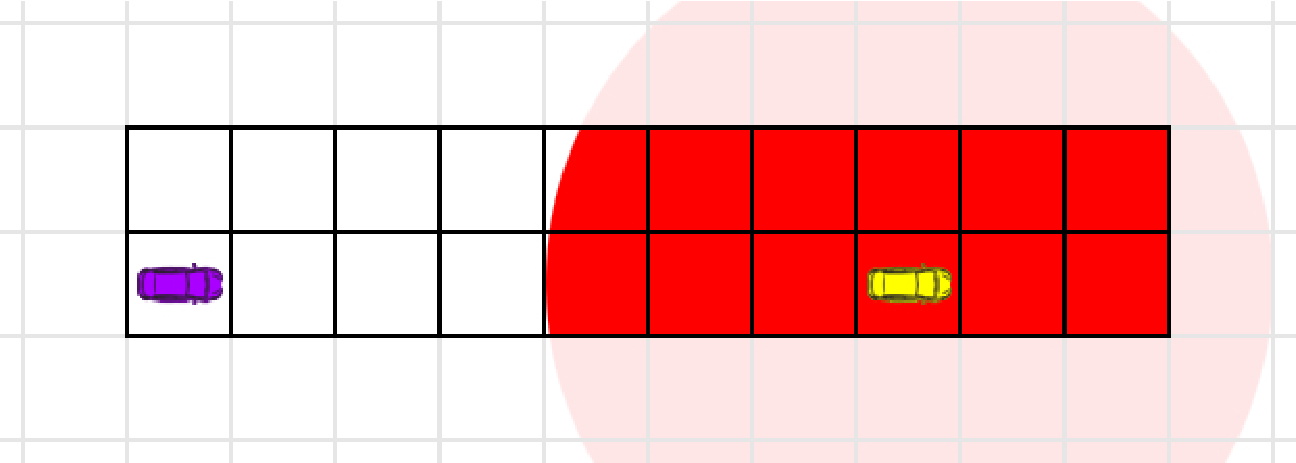
\includegraphics[width=0.8\textwidth]{view-range-no-clip}\label{figure:view-range-no-clip}} \\
    \subfigure[mit Umbruch]{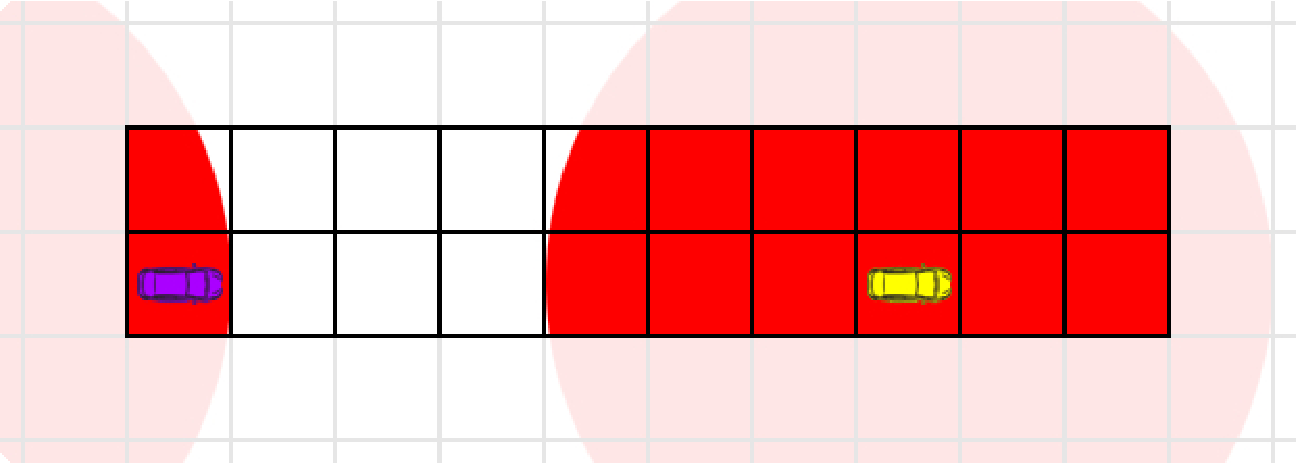
\includegraphics[width=0.8\textwidth]{view-range-clip}\label{figure:view-range-clip}}
  \caption[Umbrechen des Sichtfelds eines Fahrzeugs am Ende der Lane]
          {Sichtfeld des gelben Fahrzeugs am Ende der Lane, Quelle Auto-Silhouette: vecteezy.com}
  \label{figure:view-range-no-clip-clip}
\end{figure}

Für die Erstellung der sichtbaren Umgebung der Fahrzeuge werden die Zellen zur \enquote{view range}, die sich innerhalb der im Szenario angegebenen Entfernung befinden.
Diese werden als relative Angaben mit dem jeweiligen Fahrzeug als Mittelpunkt gespeichert und in jedem Zeitschritt auf reale Koordinaten umgerechnet.
Befindet sich dann ein anderes Fahrzeug in einer dieser Zellen, befindet es sich im Sichtfeld und eine Entfernung und Richtung wird berechnet.

Die Schwierigkeit bestand darin, die Zellen am anderen Ende der Strecke mit in die Liste der relativen Zellpositionen aufzunehmen, siehe \cref{figure:view-range-clip}, und virtuelle Zellpositionen korrekt auf reale Positionen umzurechnen.

\begin{figure}[hptb]
  \centering
    \subfigure[vorher: Durchlauf mit Fehler]{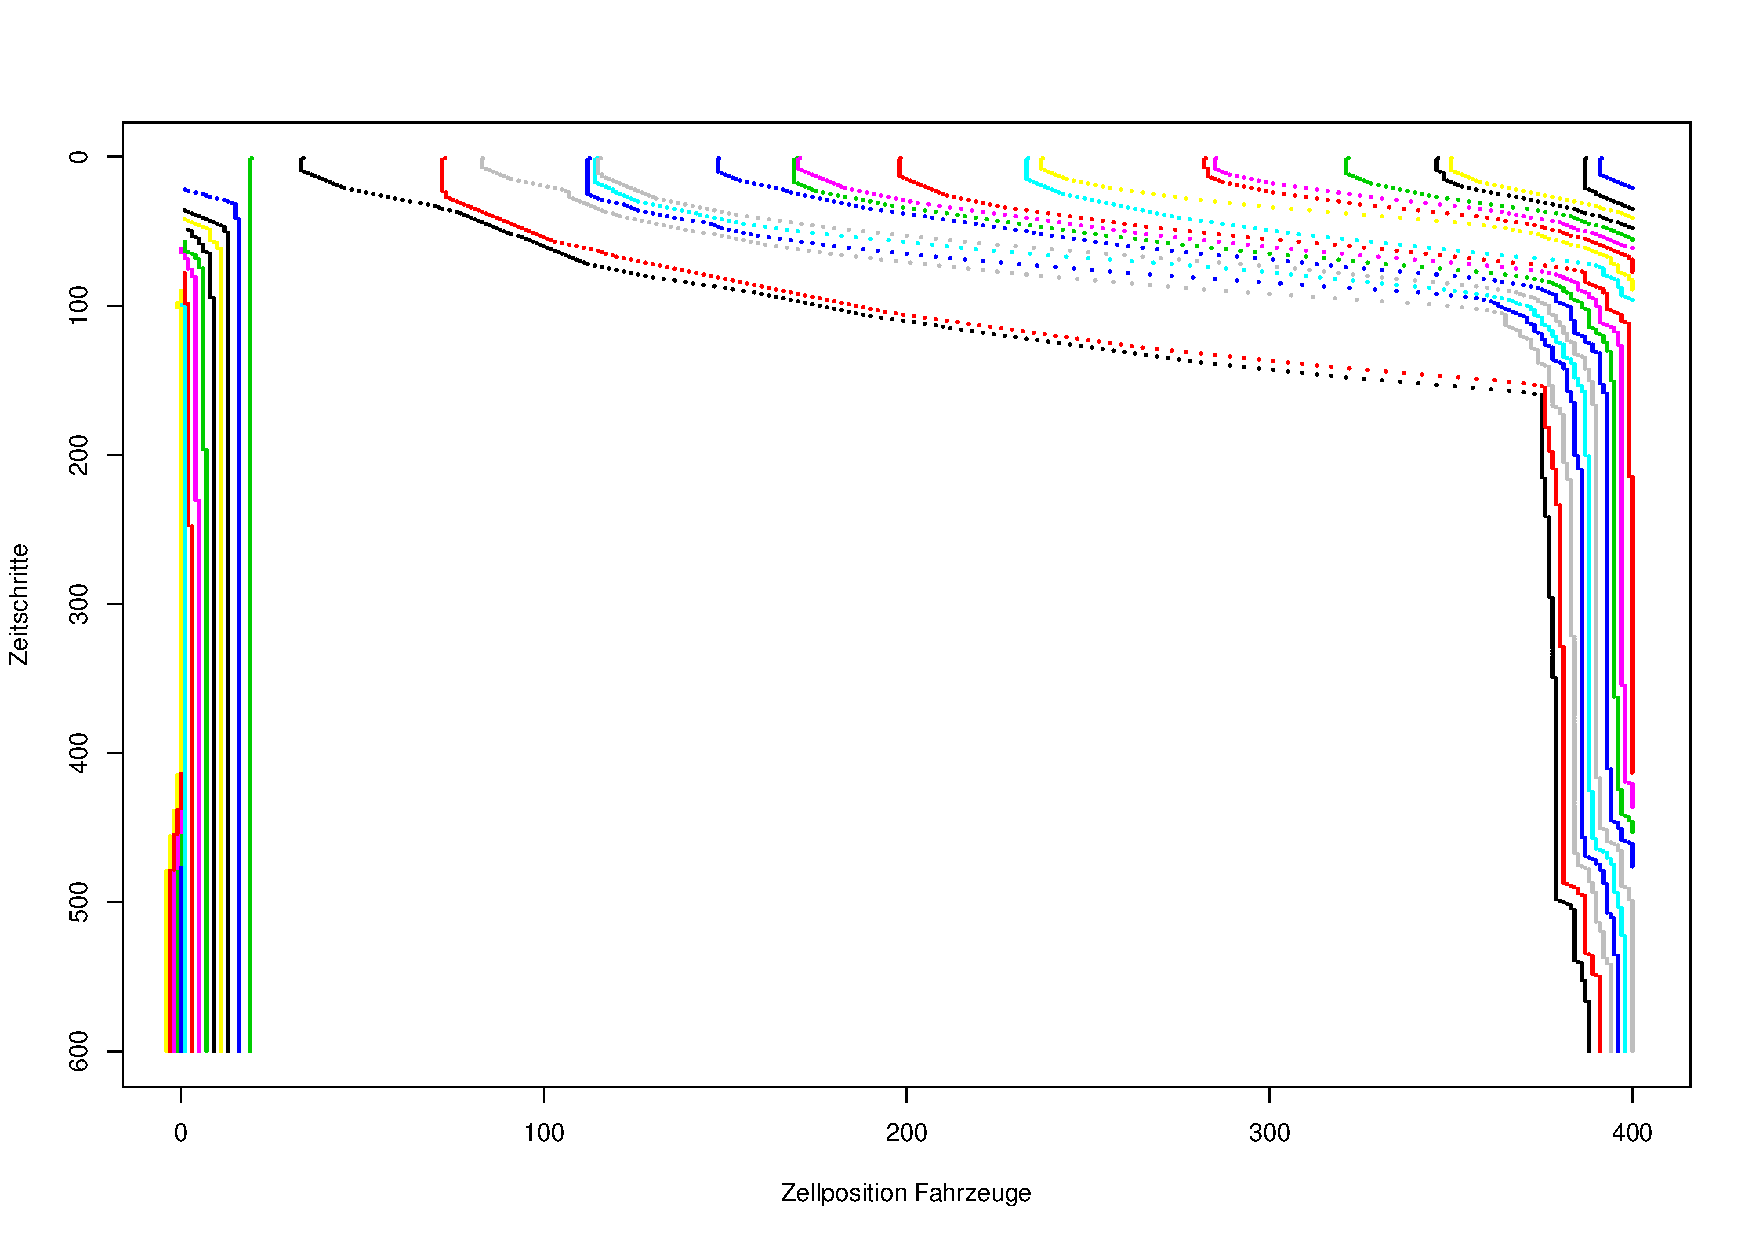
\includegraphics[width=0.45\textwidth]{go-negative_release-v175_fail}\label{figure:go-negative-fail}} \qquad 
    \subfigure[nachher: Durchlauf ohne Fehler]{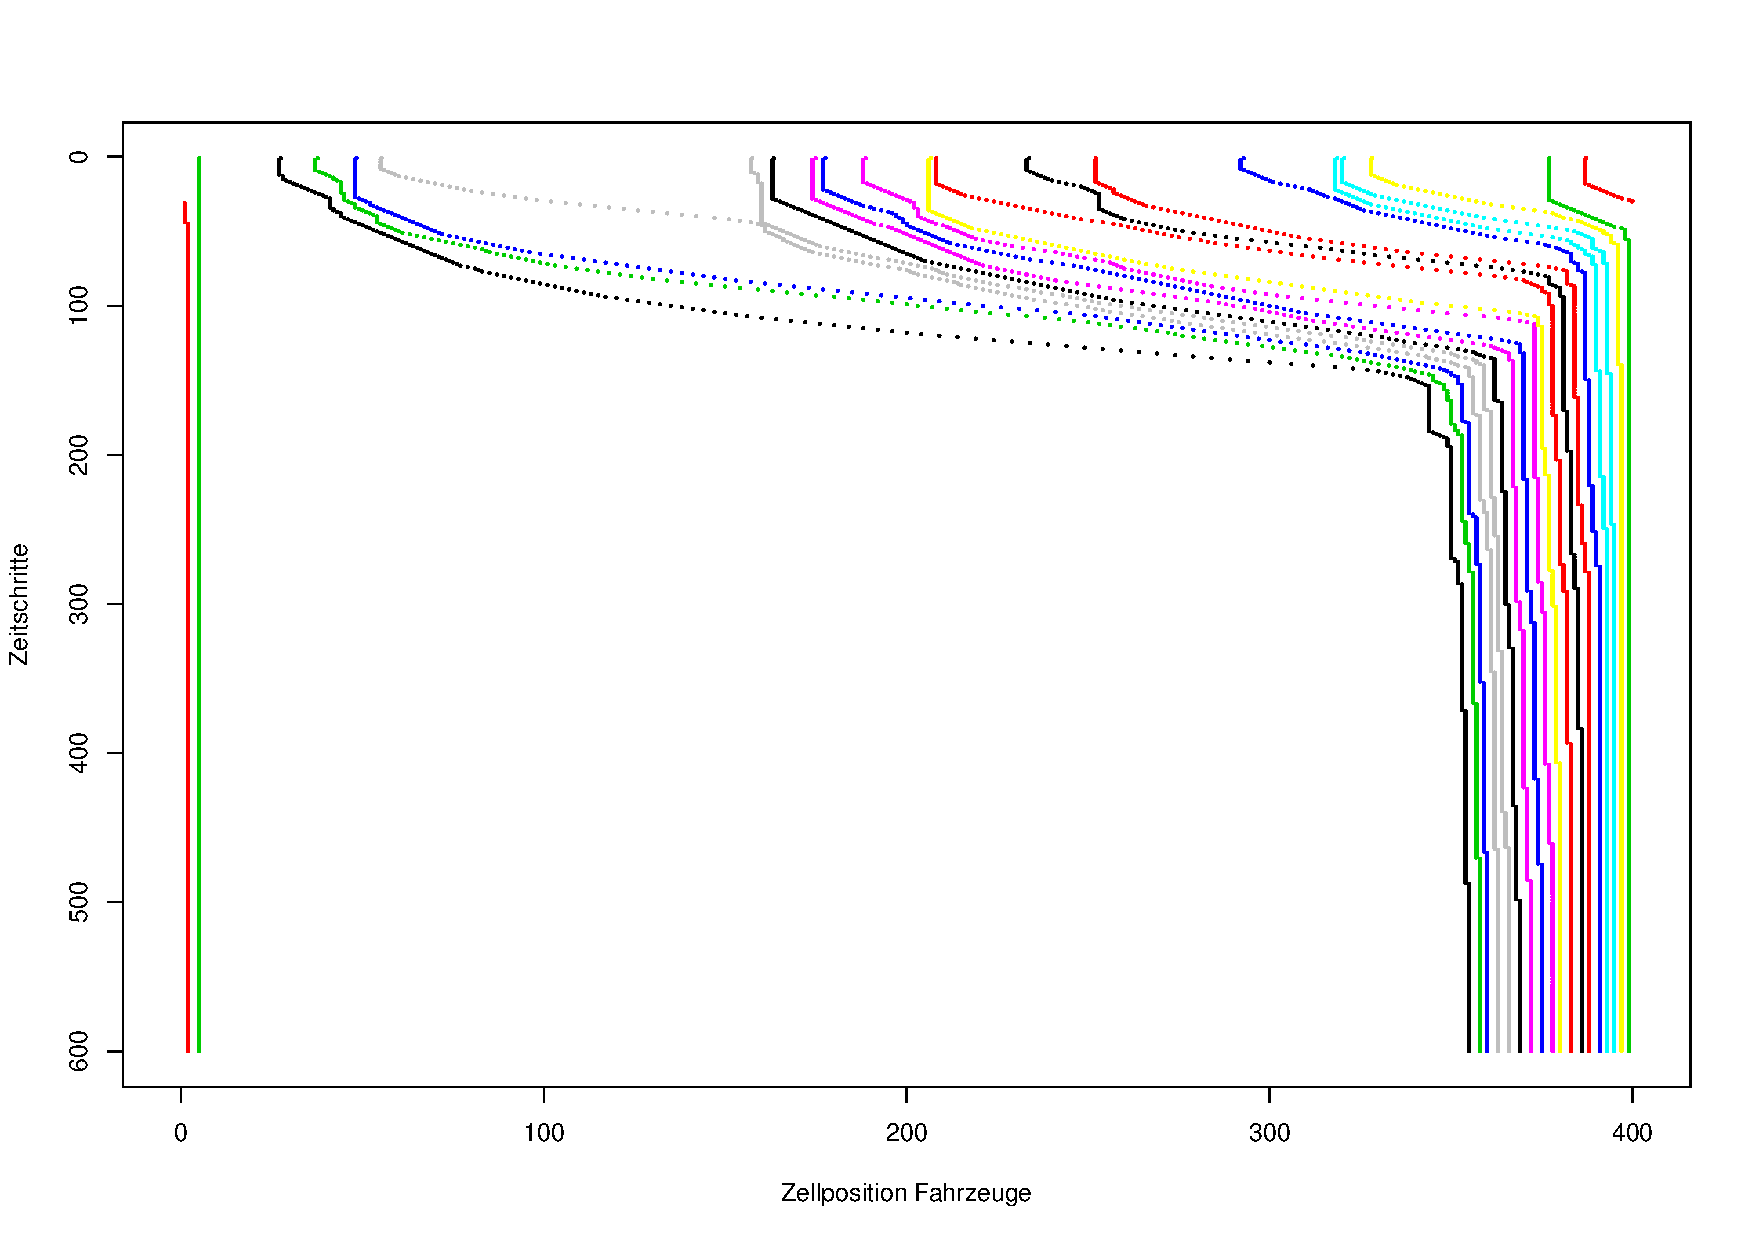
\includegraphics[width=0.45\textwidth]{go-negative_release-v185_success}\label{figure:go-negative-success}}
  \caption[Fehlerbehebung: Übergang vom Streckenende zum Anfang]
          {Fehlerbehebung des Übergangs vom Streckenende zum Anfang}
  \label{figure:go-negative}
\end{figure}

Durch Testläufe unterschiedlicher Versionen der Simulationssoftware mit identischen Szenariovorgaben - ein Fahrzeug wurde mit einer so kleinen Geschwindigkeit generiert, dass es in seiner Startzelle verblieb - konnte die Behebung des Fehlverhaltens nachgewiesen werden, siehe \cref{figure:go-negative}.

Danach konnten dann auch Stauwellen beobachtet werden, die sich rückwärts vom Streckenanfang her darüber hinaus am Streckenende fortsetzten. 



\subsubsection{Unterteilung des Sichtfeldes der Fahrzeuge}
\label{sec:unterteilung-sichtfeld}

Um die relative Position eines anderen Fahrzeugs in der Umwelt festzustellen, kann die Richtung, in der dieses sich befindet, bestimmt werden.
Die Simulationssoftware hatte für das Sichtfeld der Fahrzeuge eine Unterteilung in acht Sektoren vorgesehen, sodass neben den Richtungen vorwärts, rückwärts, links und rechts auch Unterscheidung in Zwischenschritte links vorwärts, rechts vorwärts usw. möglich war, siehe \cref{figure:car-view-8sectors}.

\begin{figure}[hptb]
  \centering 
   \subfigure[acht Sektoren]{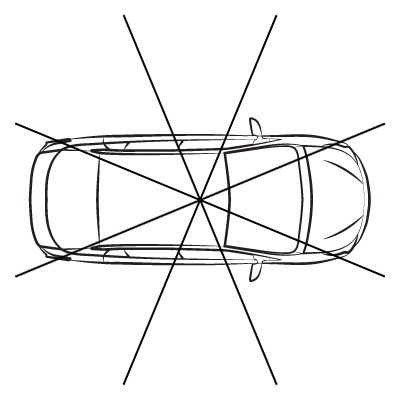
\includegraphics[width=0.3\textwidth]{car-view-8sectors}\label{figure:car-view-8sectors}}\qquad 
   \subfigure[zwei Sektoren]{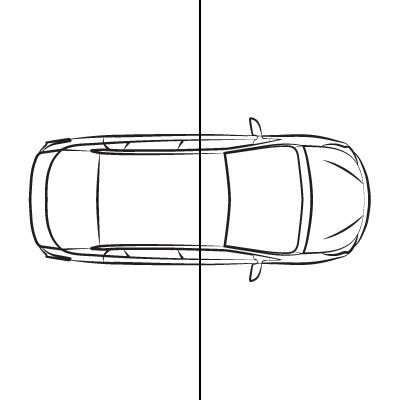
\includegraphics[width=0.3\textwidth]{car-view-2sectors}\label{figure:car-view-2sectors}}\qquad 
   \subfigure[vier Sektoren]{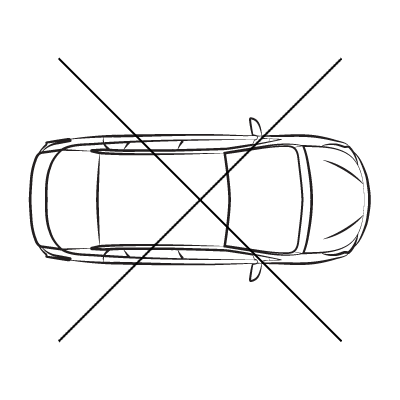
\includegraphics[width=0.3\textwidth]{car-view-4sectors}\label{figure:car-view-4sectors}}
  \caption[mögliche Unterteilung des Sichtfeldes]
          {mögliche Unterteilung des Sichtfeldes, Quelle Auto-Silhouette: vecteezy.com} 
  \label{figure:car-view-sectors}
\end{figure}

Eine solch feine Unterscheidung war nicht nötig.
Es sollte genügen, feststellen zu können, ob sich ein anderes Fahrzeug relativ zum betrachteten Fahrzeug im vorwärtigen oder rückwärtigen Raum befindet, siehe \cref{figure:car-view-2sectors}. 
Die Abdeckung der Umwelt sollte dabei ohne Unterbrechung sein.
Für die Simulation nach dem Einspurmodell von Nagel-Schreckenberg funktionierte dies ohne Probleme.

Bei einem Testlauf des Mehrspurmodells mit vier Fahrzeugen kam es allerdings zur Kollision zweier Fahrzeuge. 
Bei der Kontrolle des Logs wurde festgestellt, dass ein Fahrzeug (\texttt{vehicle0}), welches sich auf der Überholspur (lane 2) befand, ein anderes Fahrzeug (\texttt{vehicle20}) direkt neben sich nicht \enquote*{gesehen} hatte. 
Erkennbar in der Zeile \enquote{\texttt{PIA1}}, die nur ausgelöst wurde, wenn sich keinerlei Verkehr im Sichtfeld des Fahrzeuges befindet.
Es gab in dieser Konstellation demnach keine Zuordnung dieser Position zu einer der beiden Bereiche.
Daraufhin, so wie es das Verhalten des Agenten vorsah, wurde zum nächsten Schritt (366) in die Hauptspur gewechselt. 
Im diesem Zeitschritt kam es dann zum Auslösen des Kollisionsereignisses, da der Abstand zwischen \texttt{vehicle0} und \texttt{vehicle20} nicht ausreichend groß war, um das hintere Fahrzeug mit seiner aktuellen Geschwindigkeit die volle Strecke zu bewegen.

\footnotesize\begin{verbatim}
--- step 365 ----------------
         vehicle20   in lane   1   in cell   333.0   @   74.21582362319865   kph
         vehicle2   in lane   1   in cell   282.0   @   129.99324819683062   kph
         vehicle0   in lane   2   in cell   333.0   @   99.94723620551235   kph
PIA1     vehicle0   sees no traffic at all -> Pull-in
         vehicle1   in lane   1   in cell   90.0   @   130.8321253026147   kph
--- step 366 ----------------
         vehicle20   in lane   1   in cell   4.0   @   74.21582362319865   kph
         vehicle2   in lane   1   in cell   289.0   @   131.11124225593747   kph
         vehicle0   in lane   1   in cell   3.0   @   100.80986539456516   kph
TFC100   vehicle0   has vehicle in-front of -> decelerate
COS      vehicle0   STOPPED -> collision
OUT      vehicle0   -> Pull-out attempt successful
         vehicle1   in lane   1   in cell   97.0   @   130.64144521630223   kph
\end{verbatim}
\normalsize

Das Sichtfeld der Fahrzeuge wurde hierauf zu einem Vier-Sektoren-Modell abgewandelt, siehe \cref{figure:car-view-4sectors}, und die Pläne für Ein- und Ausscheren, der hiervon gleichermaßen betroffen sein dürfte, angepasst.
Es werden nun jeweils die beiden Sektoren kontrolliert, die die Bewegungs- bzw. Orientierungsrichtung darstellen. 
Nach vorn und hinten wird jeweils auch auf Entfernungen geprüft, seitlich genügt es auf reine Präsenz/Nichtpräsenz von anderen Fahrzeugen zu prüfen.

Im Rahmen dieser Umstellung wurde festgestellt, dass es bei der Richtungsbestimmung einen Fehler in der Simulationssoftware gab.
Die Berechnung lieferte für beide seitlichen Richtungen ein und denselben Wert.
Der Fehler war durch die Verwendung der Methode \texttt{acos} entstanden, wobei nicht beachtet wurde, dass der arccos nur im Bereich 0 bis $ \pi $ definiert ist, hier aber der Vollkreis zugrunde liegt.





\subsection{Entwicklung des Agentenverhaltens}
\label{sec:entwicklung-agentenplan}

Die mathematischen Gleichungen in \cite{na-sch} beschreiben gut, welches Verhalten dem Agenten zu geben ist: 
\begin{itemize}
\itemsep0em
	\item wenn möglich beschleunigen
	\item zufällige Reduktion der Geschwindigkeit (Trödeln)
	\item wenn nötig abbremsen
\end{itemize}


\subsubsection{Zustandsautomat}

Das oben beschriebene Verhalten wurde mit Hilfe eines endlichen Automaten beschrieben, siehe \cref{figure:fsm-nasch}.

\begin{figure}[hptb]
 \centering
 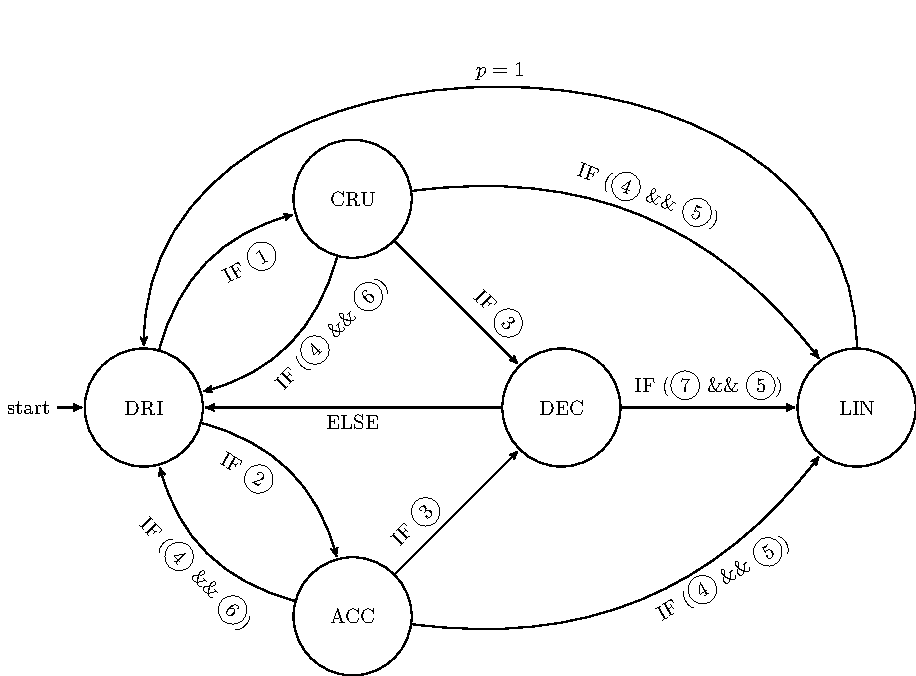
\includegraphics[width=0.9\textwidth]{fsm-nasch}
 \caption[Zustandsautomat für das Agentenverhalten]
 		{Zustandsautomat für das Agentenverhalten nach dem Nagel-Schreckenberg-Modell}
 \label{figure:fsm-nasch}
\end{figure}

Erläuterungen zu \cref{figure:fsm-nasch}:
\begin{enumerate}
\itemsep0em
	\item  $ v_{aktuell}  >=  v_{limit} $
	\item  $ v_{aktuell}  <  v_{limit} $
	\item  \enquote{Verkehr voraus}
	\item  \enquote{kein Verkehr voraus} UND $ p_{linger} $
	\item  \enquote{kein Verkehr voraus} UND $ 1 - p_{linger} $
	\item  $ v_{aktuell}  > 0 $ UND $ p_{linger} $
\end{enumerate}

Startzustand ist ein allgemeiner Zustand \texttt{DRI} (Drive/Fahren), in dem nichts am Verhalten des Agenten geändert wird.
Von hier aus ist der Zustand \texttt{ACC} (Accelerate/Beschleunigen) zu erreichen, wenn die aktuelle Geschwindigkeit unter der max. zulässigen liegt. 
Der Zustand \texttt{CRU} (Cruisen) wird erreicht, wenn die max. zulässige Geschwindigkeit erreicht oder überschritten ist.

Die Übergänge aus den zwei letztgenannten Zuständen sind identisch. 
Ist kein vorausfahrender Verkehr vorhanden und wird nicht getrödelt erfolgt der Übergang zurück in den normalen \texttt{DRI}-Zustand.
Wird stattdessen zufällig mit Wahrscheinlichkeit $ p_{linger} $ das Trödeln angestoßen, wird der entsprechende Zustand \texttt{LIN} erreicht.
Ist Verkehr voraus, wird der Zustand \texttt{DEC} (Decelerate/Verzögern, Bremsen) erreicht.

Aus dem \texttt{DEC}-Zustand kann zufällig ein Übergang in den \texttt{LIN}-Zustand erfolgen ansonsten zurück in den allgemeinen \texttt{DRI}-Zustand.
Aus dem \texttt{LIN}-Zustand wird zwangsläufig wieder in den \texttt{DRI}-Zustand übergegangen.

Ein Zeitschritt der Simulation entspricht dabei einem Zyklus vom Startzustand ausgehend bis zur Rückkehr dorthin.


\subsubsection{Agentenplan}

Der o.g. Automat wurde in die Agentensprache \enquote{übersetzt}. 
Die Agentenversion unterscheidet sich dabei leicht von der Automatenversion. 

Der Agent beginnt im Plan \enquote{\texttt{cruise}}, von dem aus alle weiteren Pläne (\enquote{\texttt{accelerate}}, \enquote{\texttt{linger}}, \enquote{\texttt{decelerate}}) gestartet werden.
Außerdem ruft sich der Plan selbst wieder auf.
\\
Während der Simulationsläufe diente dieser Plan zudem dem Loggen der Statusdaten.
Das komplette Listing siehe \cref{lst:nasch}.

\begin{minipage}[hptb]{0.95\textwidth}
\begin{lstlisting}[style=asl, 
                   keywords={!cruise}, 
                   keywords={[2]}, 
                   keywords={[3]}, 
                   caption={Auszug aus Agentenscript: single lane-Version},
                   label={lst:nasch-auszug}]      
!cruise.

// --- start all other plans ---
+!cruise <-
    !accelerate;
    !decelerate;
    !linger;
    !cruise
.\end{lstlisting}
\end{minipage}

Der \texttt{accelerate}-Plan war ursprünglich mit der Bedingung ausgestattet, dass die Beschleunigung nur erfolgen soll, wenn die aktuelle Geschwindigkeit unter der zulässigen liegt.
Hier ergab sich das Problem, dass auch bei vorwärtigem Verkehr eine Beschleunigung durchgeführt wurde und die nachfolgende Verzögerung diesen Geschwindigkeitszuwachs in jedem Zeitschritt zusätzlich abbauen musste.
Die Fähigkeit zu verzögern war entsprechend schlecht.

Abgestellt wurde dies durch den Zusatz, dass eine Beschleunigung ebenfalls ausbleiben soll, wenn sich ein Fahrzeug im vorwärtigen Sichtbereich befindet.
Mit der Vergrößerung des Sichtfeldes, siehe \cref{sec:sichtweite}, wurde es nötig, außerdem die Entfernung mit in die Bedingung aufzunehmen, ab der nicht mehr beschleunigt werden soll.

Um einen realen Folgeverkehr zu ermöglichen erfolgt die Ausnahme, dass dennoch beschleunigt werden darf, solange das Folgefahrzeug langsamer ist.

Der \texttt{linger}-Plan modelliert das zufällige Verringern der Geschwindigkeit. 
Mit einer Wahrscheinlichkeit von $10 \%$ wird das Trödeln ausgeführt.
Die Intensität der Verzögerung wurde nach einigen Tests, siehe \cref{sec:lingersweetspot}, auf den Wert \texttt{0,3}, was 30 $\%$ der Bremskraft entspricht, festgelegt.

Die Verzögerung des Agenten wird durch den \texttt{decelerate}-Plan gesteuert. 
Dort wird das Abbremsen bei vorwärtigem Verkehr geregelt. 
Auch hier wurde es nach Erweiterung des Sichtfeldes nötig, zusätzliche Bedingungen für die relative Geschwindigkeit und einen Abstand zwischen den Fahrzeugen einzufügen, um die Lücke nicht zu groß werden zu lassen und das Abbremsen nicht übermäßig stark ausfällt.

Die realistische Modellierung der Geschwindigkeitsänderungen macht es unmöglich, dass die Fahrzeuge in aufeinanderfolgenden Zellen hinterher fahren.
Vielmehr muss, wie im realen Verkehr auch, ein gewisser Abstand, innerhalb dessen der Nachfolgeverkehr reagieren kann, eingehalten werden.
Ein Wert von 100 m erschien in der Simulation sinnvoll, um die Kollisionshäufigkeit zu verringern. 
Für eine Geschwindigkeit von 100 km/h entspricht diese Entfernung nach der Faustformel, siehe \cite{bremsweg}, dem Bremsweg.

Ist der Geschwindigkeitsunterschied zwischen Fahrzeugen allerdings zu groß, können diese nicht verhindert werden.

\paragraph*{Tests des Agentenplanes}
Um die Wirksamkeit der Anweisungen für die Agenten zu testen, wurden in der Szenarienvereinbarung zwei Arten von Fahrzeugen, welche mit identische Plänen ausgestattet waren, zum Einsatz gebracht.
Der einzige Unterschied, den es zwischen den Fahrzeugen gab, war, dass eines seine Geschwindigkeit aus einem niedrigeren Intervall zugewiesen bekam.
\\
Somit war sichergestellt, dass das schnellere Fahrzeug im Laufe der für Testzwecke kurz gehaltenen Simulationzeit auf das langsamere aufholen würde.
Es war wiederholbar zu testen, ob das Abbremsen bei vorwärtigem Verkehr funktionierte.

\sa{own: [Grafik Speedcurve][Grafik Cellcurve]}
%\begin{figure}[hptb]
%  \centering 
%   \subfigure[Zellpostionen]{\includegraphics[width=0.5\textwidth]{image1name}\label{figure:image1name}}\qquad 
%   \subfigure[Geschwindigkeit]{\includegraphics[width=0.5\textwidth]{image2name}\label{figure:image2name}}
%  \caption{lalala} 
%  \label{figure:imagename}
%\end{figure}






\subsection{Verfeinerung des Agentenverhaltens}
\label{sec:verfeinerung-agentenplan}

Das Szenario für die Simulation kann über eine YAML-Datei individuell eingestellt werden.
Es gibt u.a. die Möglichkeit, die Streckenlänge und die Simulationsdauer, die Zellgröße und die Zeitschrittgröße und über Intervalle die Geschwindigkeit und die Beschleunigungs- und Verzögerungswerte der Fahrzeuge anzugeben.



\subsubsection{Einstellmöglichkeiten in der Szenarienkonfiguration}
\label{einstellungen-szenario}

%\subsubsection{Einstellmöglichkeiten für Zellgröße und Länge der Zeitschritte}

\paragraph*{Zellgröße:}
\label{zellgroesse-zeitschritte}
Die Entwicklung der Agentenpläne wurde ausschließlich in einer Simulationsumgebung mit einer Zellgröße von 7,5 m durchgeführt.
Als das Verhalten der Agenten zufriedenstellend war, wurde u.a. auch wegen der in \cref{sec:bremsverhalten} angemerkten Bremsprobleme, getestet, inwiefern sich die Zelllänge verkürzen lässt und welchen Einfluss dies auf die Simulation hat.

% --- für Ausblick, Phil FB 27feb
% --- war vorerst nur solala formuliert
%Bei der Aufgrund der Parallelausführung der Simula-
%tion ergeben sich für die Entscheidungsgrundlagen der einzelnen Agenten unterschiedliche Vor-
%aussetzungen. Ein Fahrzeug sah z.B. regelmäßig die Position eines anderen Fahrzeugs aus dem
%vorangegangenen Zeitschritt und musste aufgrund dieser Informationen handeln. Hier konnten
%z.B. kritische Situationen nicht erkannt werden.

\paragraph*{Zeitschrittlänge:}
Die Länge der Zeitschritte lässt sich in der Konfiguration in Minuten oder Bruchteilen davon angeben. 
Dies stellte sich als unpraktikabel heraus, da z.B. eine Dauer von einer Sekunde durch den Dezimalbruch für $\frac{1}{60}$ angegeben werden müsste, der aber eine Periodizität aufweist.

Begonnen wurde mit einer Zeitschrittlänge von 0,1 min, was sechs Sekunden entspricht. 
Diese Länge erwies sich als nicht sinnvoll, da zwischen den einzelnen Entscheidungszeitpunkten eine zu lange Zeitspanne liegt.

Die Entwicklung der Agentenpläne wurde mit einer Schrittlänge von drei Sekunden, 0,05 min, durchgeführt und genügte für diesen Zweck völlig.
Für die Tests auf Leistungsfähigkeit wurde die Schrittlänge dann auf 0.025 min, 1,5 Sekunden, reduziert.
\\
Ausführlich siehe \cref{setup-multilane-scenarios}.


%\subsubsection{Festlegen der Beschleunigungs-/Verzögerungswerte und der Sichtweite}

\paragraph*{Beschleunigung/Verzögerung:}
\label{beschl-verz}
Das originale Modell von Nagel und Schreckenberg legt Beschleunigung, Verzögerung und Sichtweite sehr einfach fest.
Bedingt durch die Zellgröße von \mbox{7,5 m}, die Ganzzahligkeit der Geschwindigkeit und die Zeitschrittlänge von 1 Sekunde ergeben sich Beschleunigungswerte von 7,5 $\frac{m}{s^{2}}$. 
Durch die Möglichkeit, die Geschwindigkeit innerhalb eines einzigen Zeitschrittes von der Maximalgeschwindigkeit \enquote{5} auf Null zu verringern, ergibt sich theoretisch eine Verzögerung von \mbox{37,5 $\frac{m}{s^{2}}$}.
Dies ist unrealistisch.

Die Simulationsumgebung arbeitet hier mit frei wähl- und einstellbaren Werten. 
In \cite{unfallrekonstruktion} sind die Werte für eine Vielzahl von Fahrzeugen aufgelistet. 
Für die Simulation wurden real möglichen Werte zwischen 3,5 und \mbox{7 $\frac{m}{s^{2}}$} für die Beschleunigung und zwischen 8 und \mbox{10 $\frac{m}{s^{2}}$} für die Verzögerung gewählt.
Der Wert wird für jedes Fahrzeug bei der Initialisierung im Rahmen dieser Intervalle zufällig festgelegt.
Die Dosierung der möglichen Beschleunigung bzw. Verzögerung wird im Agentenscript festgelegt.

\paragraph*{Sichtweite:}
\label{sec:sichtweite}
Für die Sichtweite ergibt sich für im NaSch-Modell der theoretische Wert von \mbox{$ 5 \times $ 7,5 m}, also 37,5 Meter (bzw. je nach max. möglicher Geschwindigkeit  $ v_{max} $: \mbox{$ v_{max} \times $ 7,5 m}).
\\
Für die in der Agentensimulation vorliegenden \enquote{realen} Bremsvorgänge ist diese Entfernung unzureichend. 

Die Sichtweite im Straßenverkehr kann laut \cite{sichtweite} aufgrund von physiologischen und psychologischen Gründen in drei Zonen eingeteilt werden:
\begin{itemize}
\itemsep0em
	\item \enquote{Fernorientierung/Information}, auf Autobahnen etwa zwischen 600 und 360 Metern
	\item \enquote{Bereitschaft/Entscheidung}, etwa zwischen 360 und 110 Metern
	\item \enquote{Nahorientierung/Handlung}, unter 110 Metern
\end{itemize}

Durch die fehlende Reaktionsträgheit, die maßgeblich durch die menschliche Komponente auftritt, hier aber fehlt, muss nicht die Phase der Fernorientierung ausgeschöpft werden. 
Ein Wert der Sichtweite mittig im Intervall der Entscheidung genügt, um bis zum Beginn der Handlungsphase \enquote{tätig zu werden}.

Für die Sichtweite wurde der Wert 250 m gewählt.
Dieser liegt ungefähr mittig im Intervall der Entscheidungsphase und sollte den Agenten genügend Raum für Reaktionen geben. 
In den Agentenplänen wird schließlich die Handlung durch Bedingungen auf einen Bereich unter 110 m beschränkt.


\subsubsection{Einstellmöglichkeiten im Agentenverhalten (Parameter)}

\paragraph*{Festlegen der Trödelparameter:}
\label{sec:lingersweetspot}

Im Originalmodell wird dem jeweiligen Fahrzeug im Trö"-del"-fall eine Geschwindigkeitseinheit wieder abgezogen. 
In jenem Zeitschritt erfolgt somit keine Beschleunigung, bzw. bei Fahren mit max. möglicher Geschwindigkeit wird diese reduziert. 
Auf das Abbremsen vor einem Hindernis hat dies keinen Einfluss, weil die mögliche Geschwindigkeit an Größe der vorhandenen Lücke angepasst wird.

Für die Simulation musste ein Wert gefunden werden, der dieses Verhalten näherungsweise nachbildet.
Im Laufe mehrerer Testdurchgänge schien eine Intensität der Verzögerung von \texttt{0,3} die getätigte Beschleunigung am besten zu egalisieren. 
Hierbei ist noch die Streuung der Be"-schleu"-ni"-gungs- und Verzögerungswerte zu beachten, sodass das Trödeln unterschiedlich große Effekte haben kann.

Für das Abbremsen in der Agentensimulation kann sich das Trödeln positiv auf den Bremsweg auswirken, da ein zusätzlicher Bremsimpuls erzeugt wird. 
Hier wird im allgemeinen aber im Summe eine Verzögerung über dem max. möglichen Wert erziehlt.
\\
Aufgrund der \enquote{Bremsprobleme}, siehe \cref{sec:bremsverhalten}, wurde dies aber vorerst in Kauf genommen.

Für die Trödelwahrscheinlichkeit $ p_{linger} $ wurde beobachtet, dass deren Höhe kaum einen Einfluss auf das Verhalten bei max. möglicher Geschwindigkeit hatte.
Bei den Geschwindigkeitsreduktionen glichen sich Stärke und Muster.
//
Eine signifikante Veränderung trat jedoch bei der Beschleunigung der Fahrzeuge auf.
Je höher die Wahrscheinlichkeit desto flacher wird der Anstieg bei der Beschleunigung.
Die Verzögerungen in dieser Simulationsumgebung treten weniger wegen des Geschwindigkeitsverlustes auf, sondern wegen der Verlängerung der Zeit wieder zur ursprünglichen Geschwindigkeit zurückzukehren.
\sa{own: add 3 linger speed graphs 0,3 0,5 0,7}

Weiterhin hat die Trödelwahrscheinlichkeit bei gleicher Höhe, abhängig von gefahrenen Geschwindigkeiten, unterschiedliche Einflüsse auf den Verkehrsfluss.
\\
Bei einer max. möglichen Geschwindigkeit von 50 km/h erzeugt erst eine Wahrscheinlichkeit von \texttt{0,5} einen merklichen Effekt. Für eine Geschwindigkeit von 100 km/h ist dies bei gleicher Fahrzeuganzahl bereits bei einem Wert von \texttt{0,3} der Fall.
\\
Bei Werten darüber hinaus wurde beobachtet, dass die Beschleunigung eines oder mehrerer Fahrzeuge so gehemmt wurde, dass ein Erreichen der möglichen Geschwindigkeit für alle im System befindlichen Fahrzeuge nicht möglich war.

Für die Dauertests mit einer max. möglichen Geschwindigkeit von 100 km/h wurden die Parameter im \texttt{linger}-Plan somit auf Wahrscheinlichkeit von \texttt{0,3} und eine Bremsintensität von \texttt{0,3} festgelegt.





\subsection{Festlegen des Setups für die Langzeittests}
\label{setup-multilane-scenarios}

Den nachfolgenden Ausführungen liegt das hier beschriebene Szenario zugrunde:
\begin{itemize}
\itemsep0em
	\item Anzahl Lanes: 1
	\item Streckenlänge: 1 km
	\item Simulationsdauer: 30 min
	\item Anzahl Fahrzeuge: 2
	\item max. zulässige Geschwindigkeit: 100 km/h
	\item Trödelwahrscheinlichkeit: 0,1
\end{itemize}
Mit dem bereits erwähnten Vorgehen - identische Agentenpläne, unterschiedliches Geschwindigkeitsintervall bei der Initialisierung ($ Fzg^{S} $ = schnelleres Fahrzeug (rote Kurve), $ v \in [80; 130] $, $ Fzg^{L} $ = langsameres Fahrzeug (schwarze Kurve), $ v \in [70; 90] $) - wurde das Verhalten der Agenten, ausgehend von einer Zellgröße von 7,5 Metern (in 2,5 m-Schritten absteigend) und einer Zeitschrittgröße von 0,1 Minuten (jew. halbiert), in jew. drei Durchgängen getestet.

Für die Auswertung, ob eine Zellgröße/Zeitschrittlänge-Kombination für eine Simulationsdurchführung nutzbar ist, wurde der Ausdruck der Geschwindigkeiten der beiden Fahrzeuge über die Simulationszeit genutzt.


\subsubsection{Zellgröße 7,5 m}

\begin{figure}[hptb]
  \centering 
   \subfigure[1. Durchlauf]{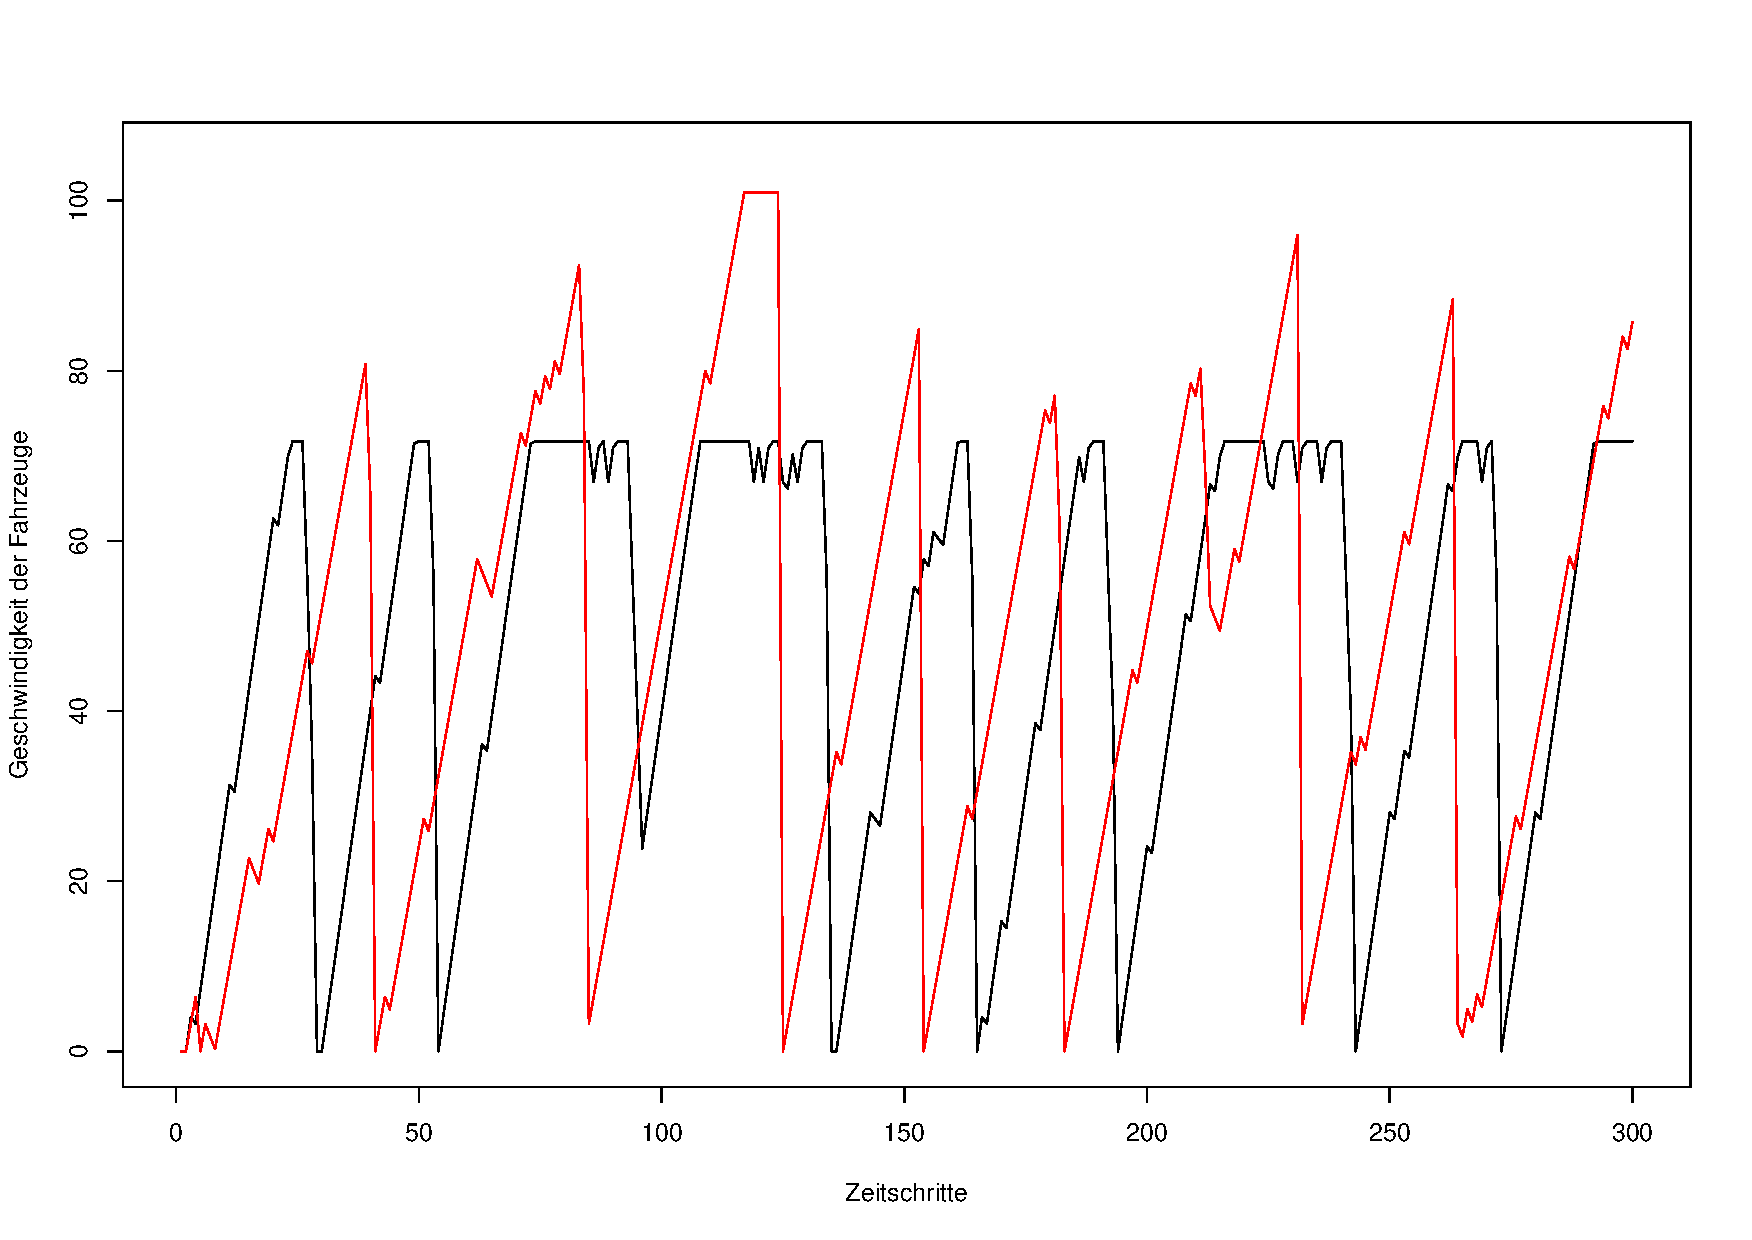
\includegraphics[width=0.3\textwidth]{speed_run1}\label{figure:run1}}\qquad 
   \subfigure[2. Durchlauf]{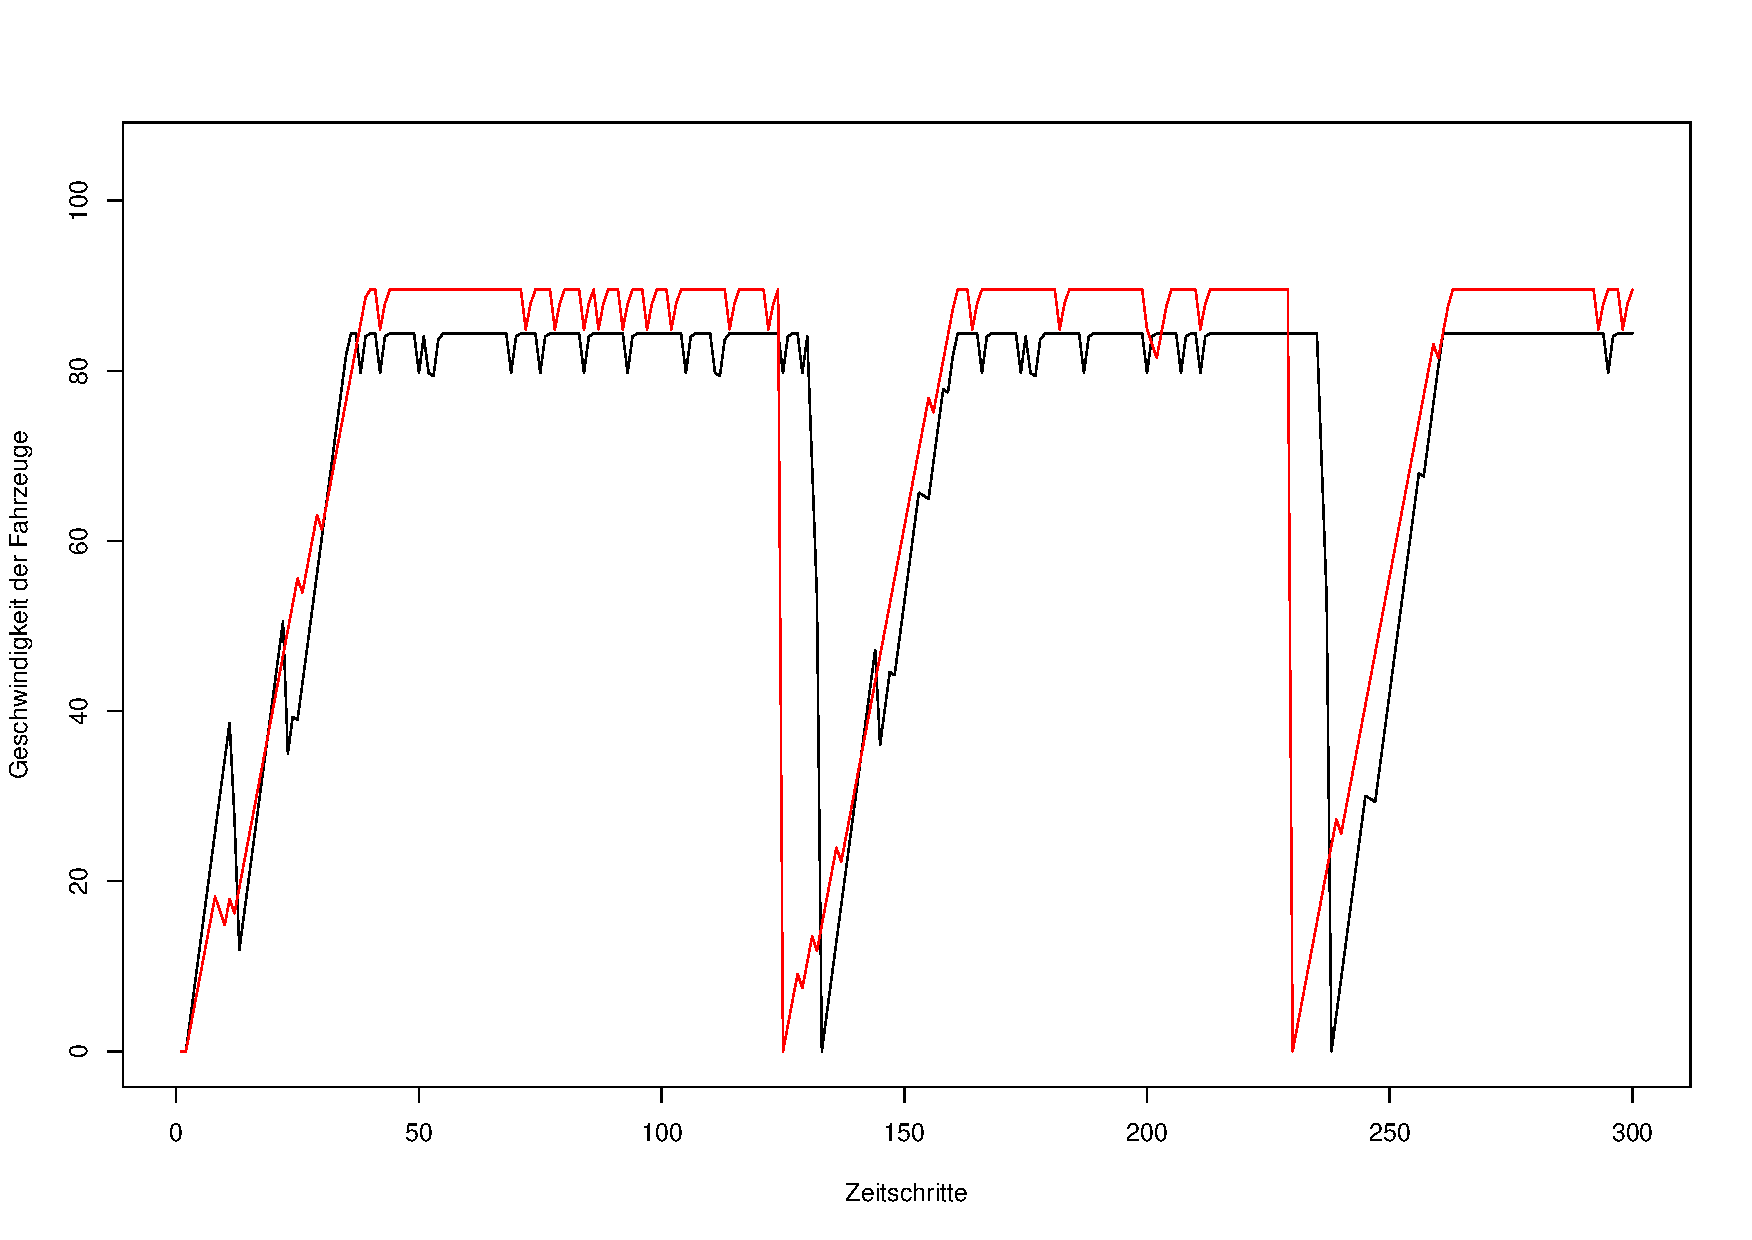
\includegraphics[width=0.3\textwidth]{speed_run2}\label{figure:run2}}\qquad 
   \subfigure[3. Durchlauf]{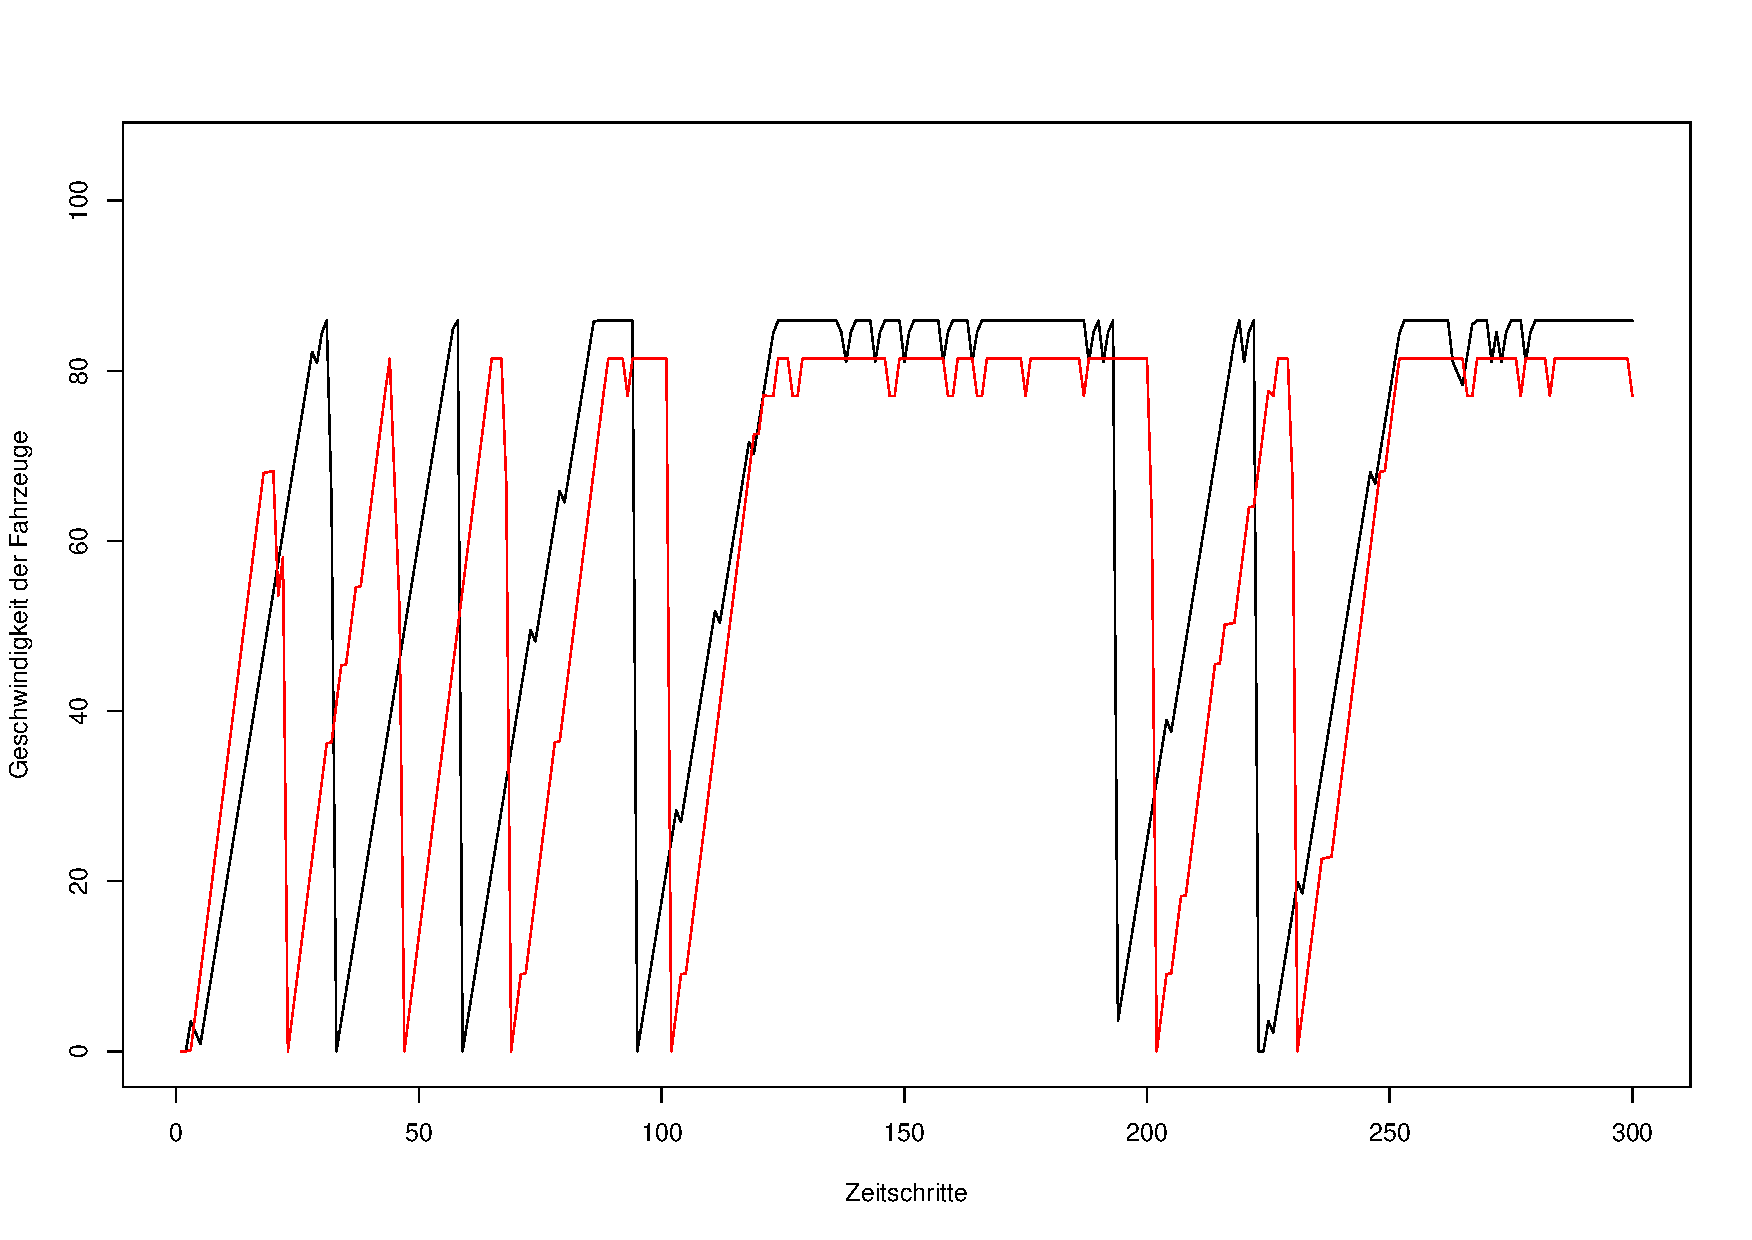
\includegraphics[width=0.3\textwidth]{speed_run3}\label{figure:run3}}
  \caption{Simulationen mit Zellgröße 7,5 m und Zeitschrittlänge 0,1 min} 
  \label{figure:run1-3}
\end{figure}

In allen drei Kurvenverläufen in \cref{figure:run1-3} sind mehrfach Reduktionen der Geschwindigkeit auf Null zu sehen. 
Dies zeigt, dass an diesen Stellen eine Kollision stattgefunden hat. Das Kollisionsereignis wird vom Simulationstool ausgelöst, wenn ein Fahrzeug nicht in der Lage wäre, im nächsten Zeitschritt die für seine Geschwindigkeit entsprechende Streckenlänge zurückzulegen.

Die Zeitschrittlänge von 0,1 Minuten, was sechs Sekunden entspricht, ist nicht ausreichend, um Geschwindigkeit in ausreichendem Maße abzubauen, um genug Abstand vom Vordermann einzuhalten.

Auf die Ausführung von Durchgängen mit dieser Zeitschrittgröße und kleinerer Zellgröße wurde verzichtet.

\begin{figure}[hptb]
  \centering 
   \subfigure[1. Durchlauf]{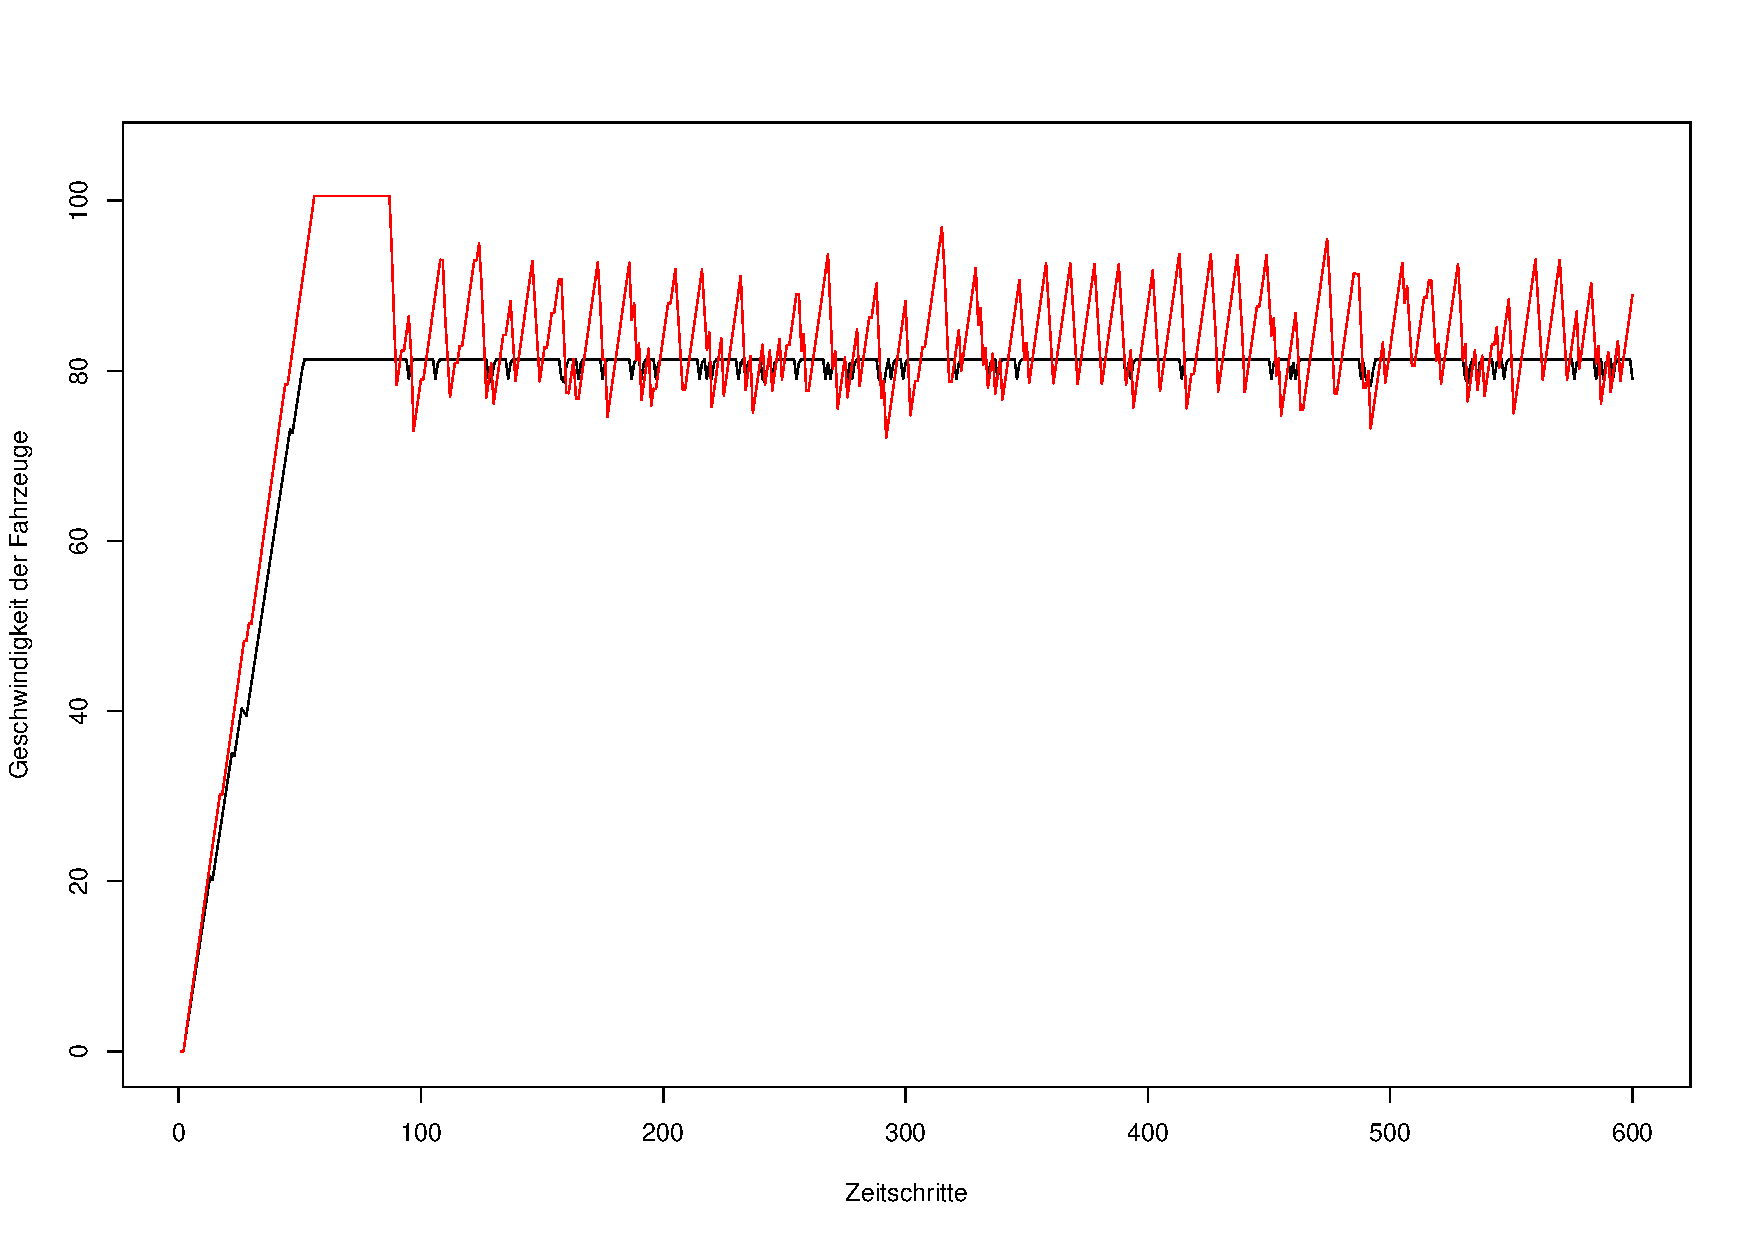
\includegraphics[width=0.3\textwidth]{speed_run4}\label{figure:run4}}\qquad 
   \subfigure[2. Durchlauf]{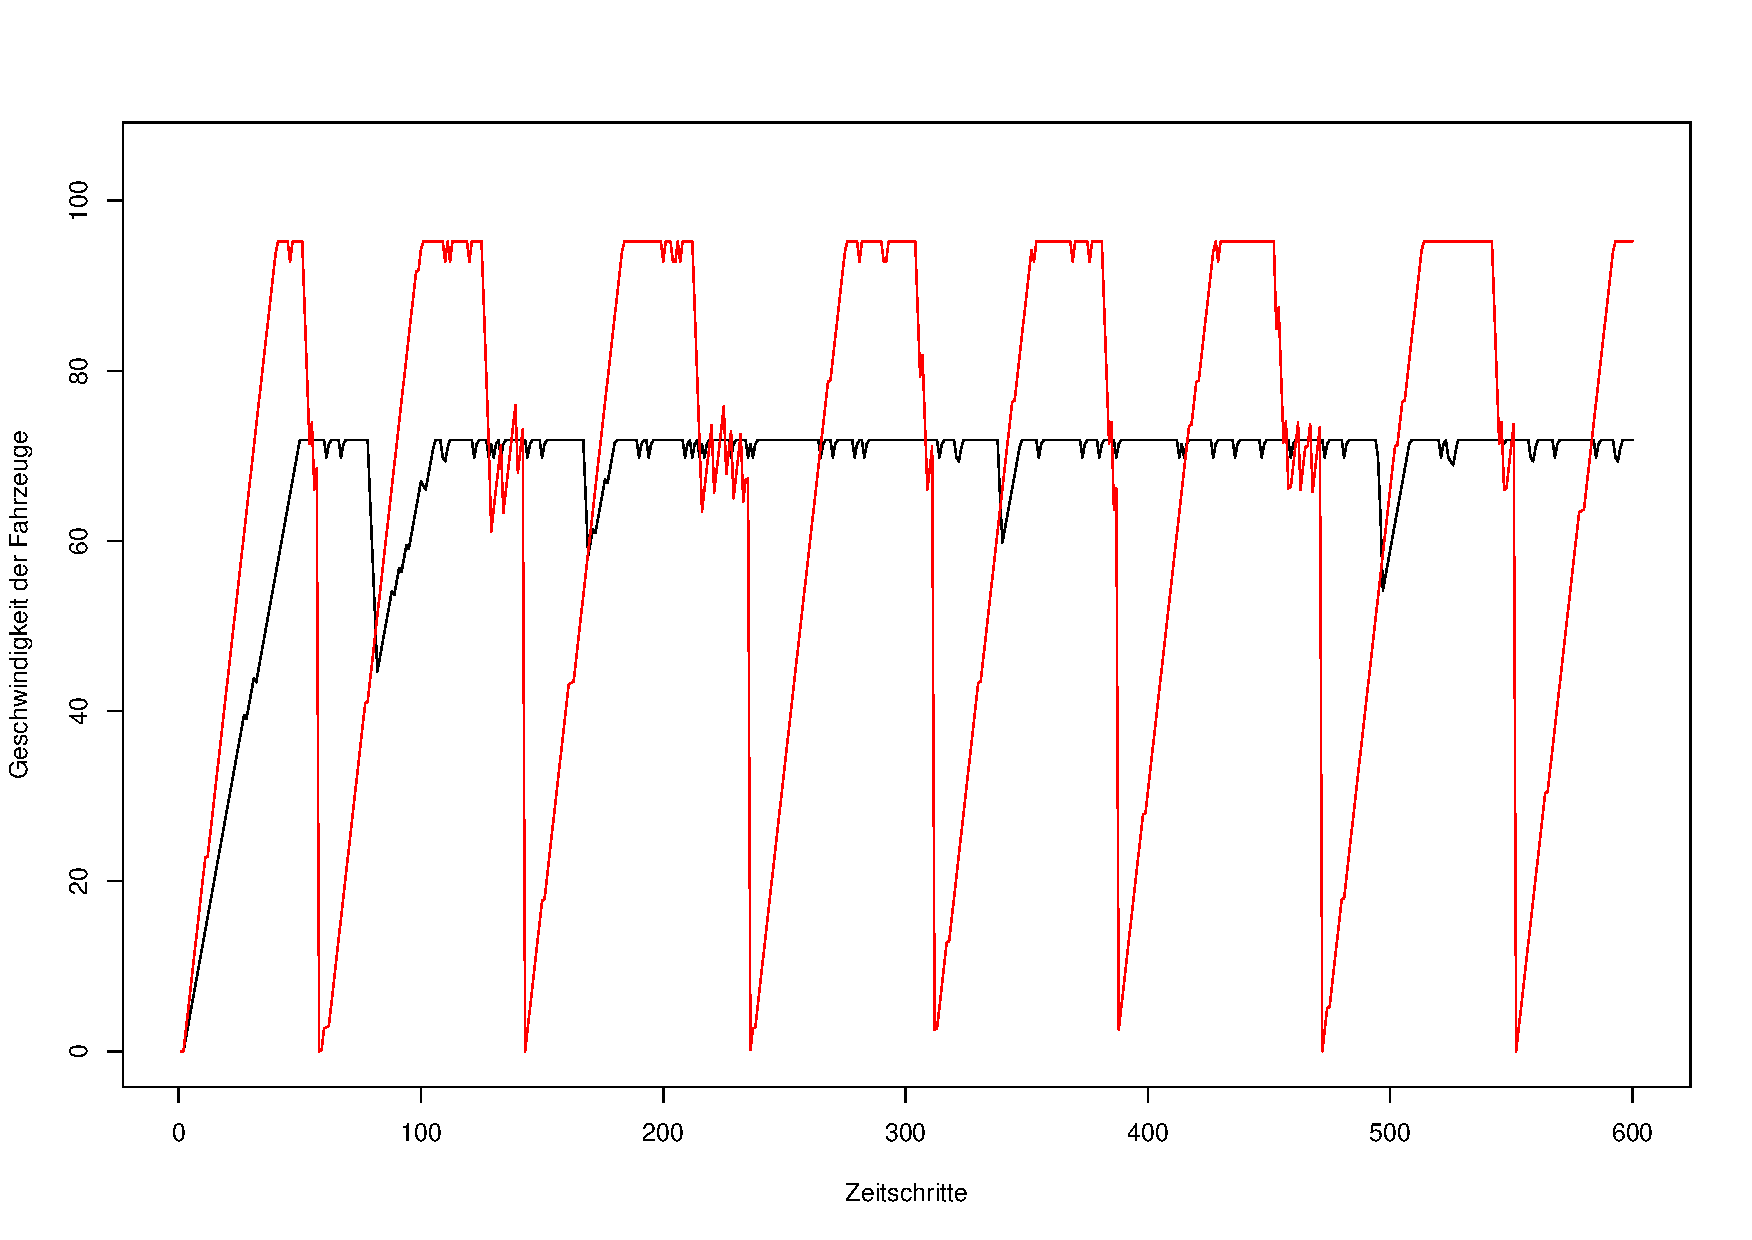
\includegraphics[width=0.3\textwidth]{speed_run5}\label{figure:run5}}\qquad 
   \subfigure[3. Durchlauf]{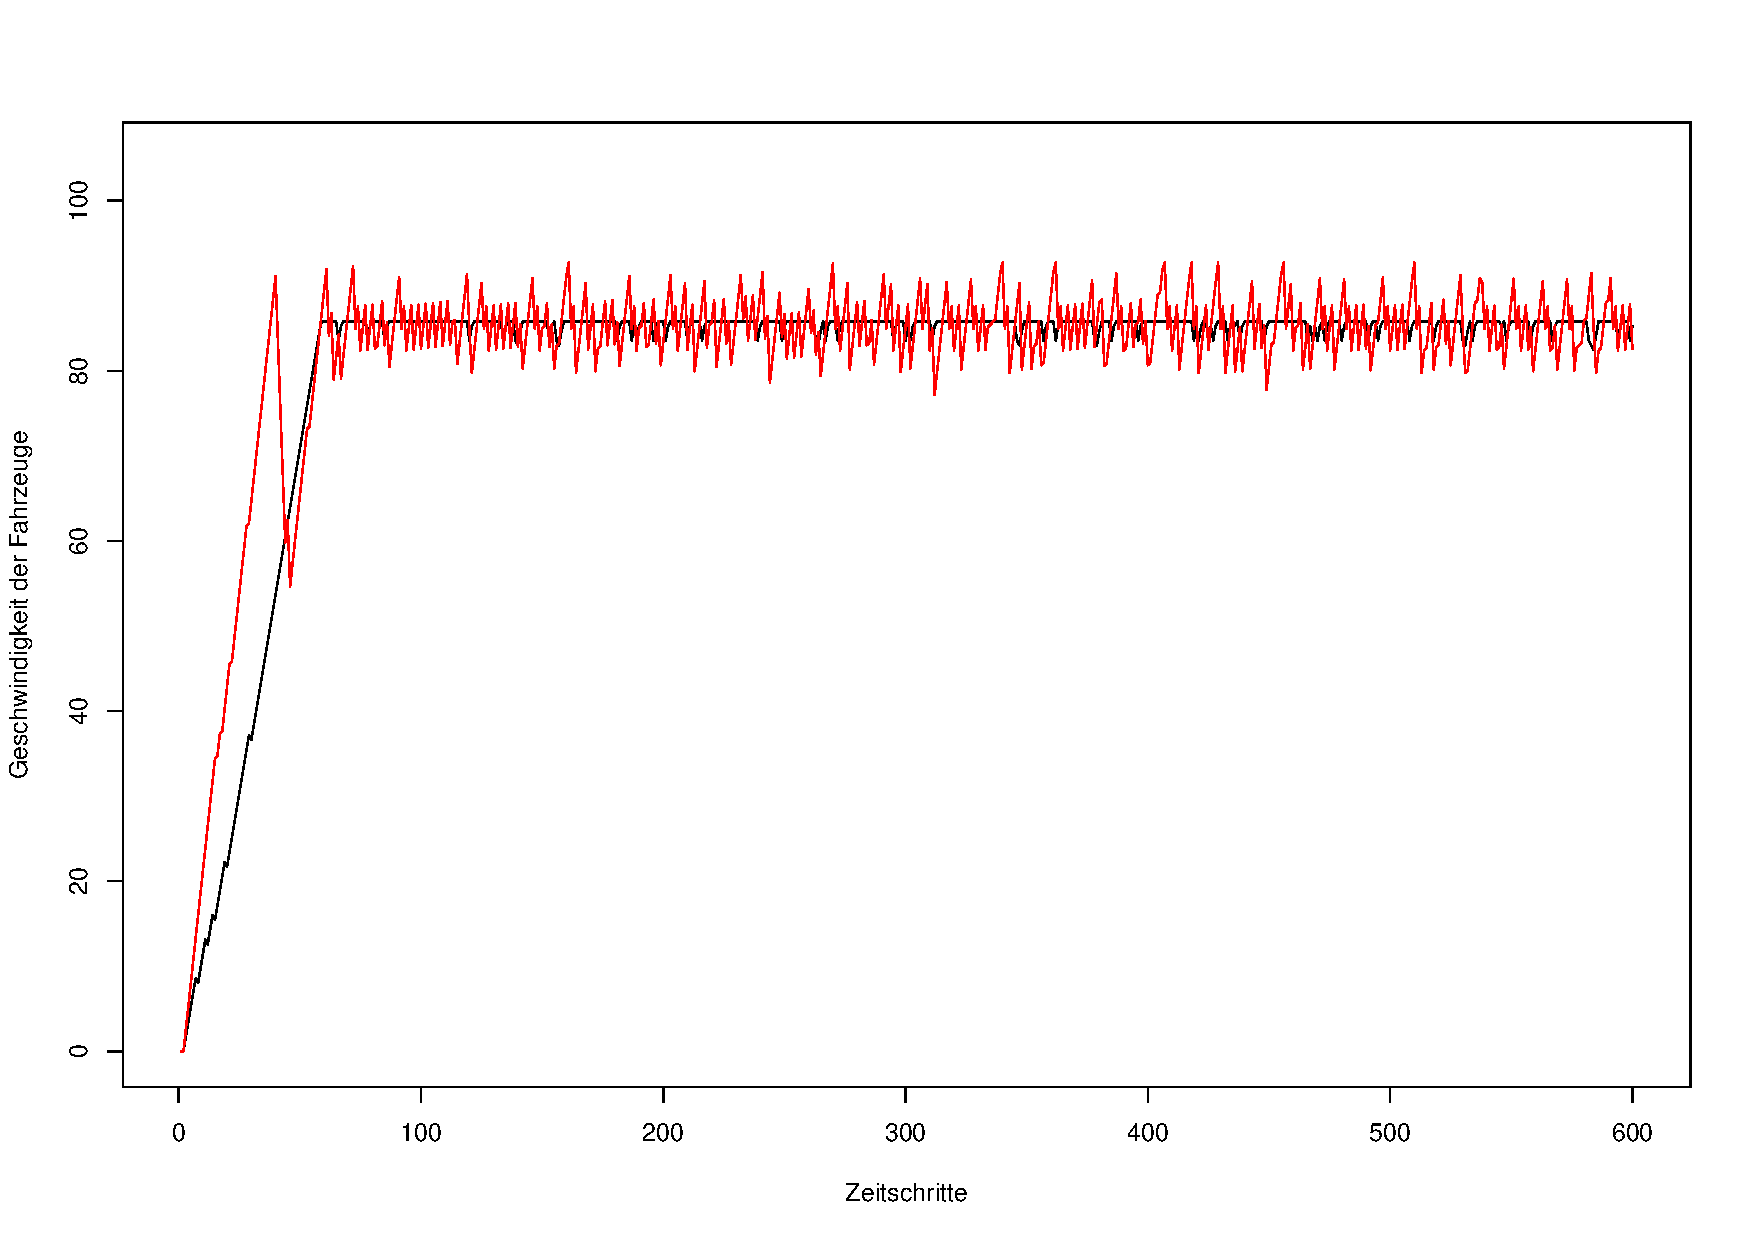
\includegraphics[width=0.3\textwidth]{speed_run6}\label{figure:run6}}
  \caption{Simulationen mit Zellgröße 7,5 m und Zeitschrittlänge 0,05 min} 
  \label{figure:run4-6}
\end{figure}

Die Verläufe der Kurven in \cref{figure:run4-6} zeigen in zwei von drei Fällen, dass sich die Geschwindigkeit des auffahrenden Fahrzeuges um die des langsameren Fahrzeuges einpendelt.

Im Plot des zweiten Durchlaufes ist zu sehen, dass auch in dieser Konstellation Kollisionen stattgefunden haben.
Die Geschwindigkeit des langsameren Fahrzeuges lag in diesem Durchlauf im Vergleich zu den anderen beiden um einiges niedriger.

\begin{figure}[hptb]
  \centering 
   \subfigure[1. Durchlauf]{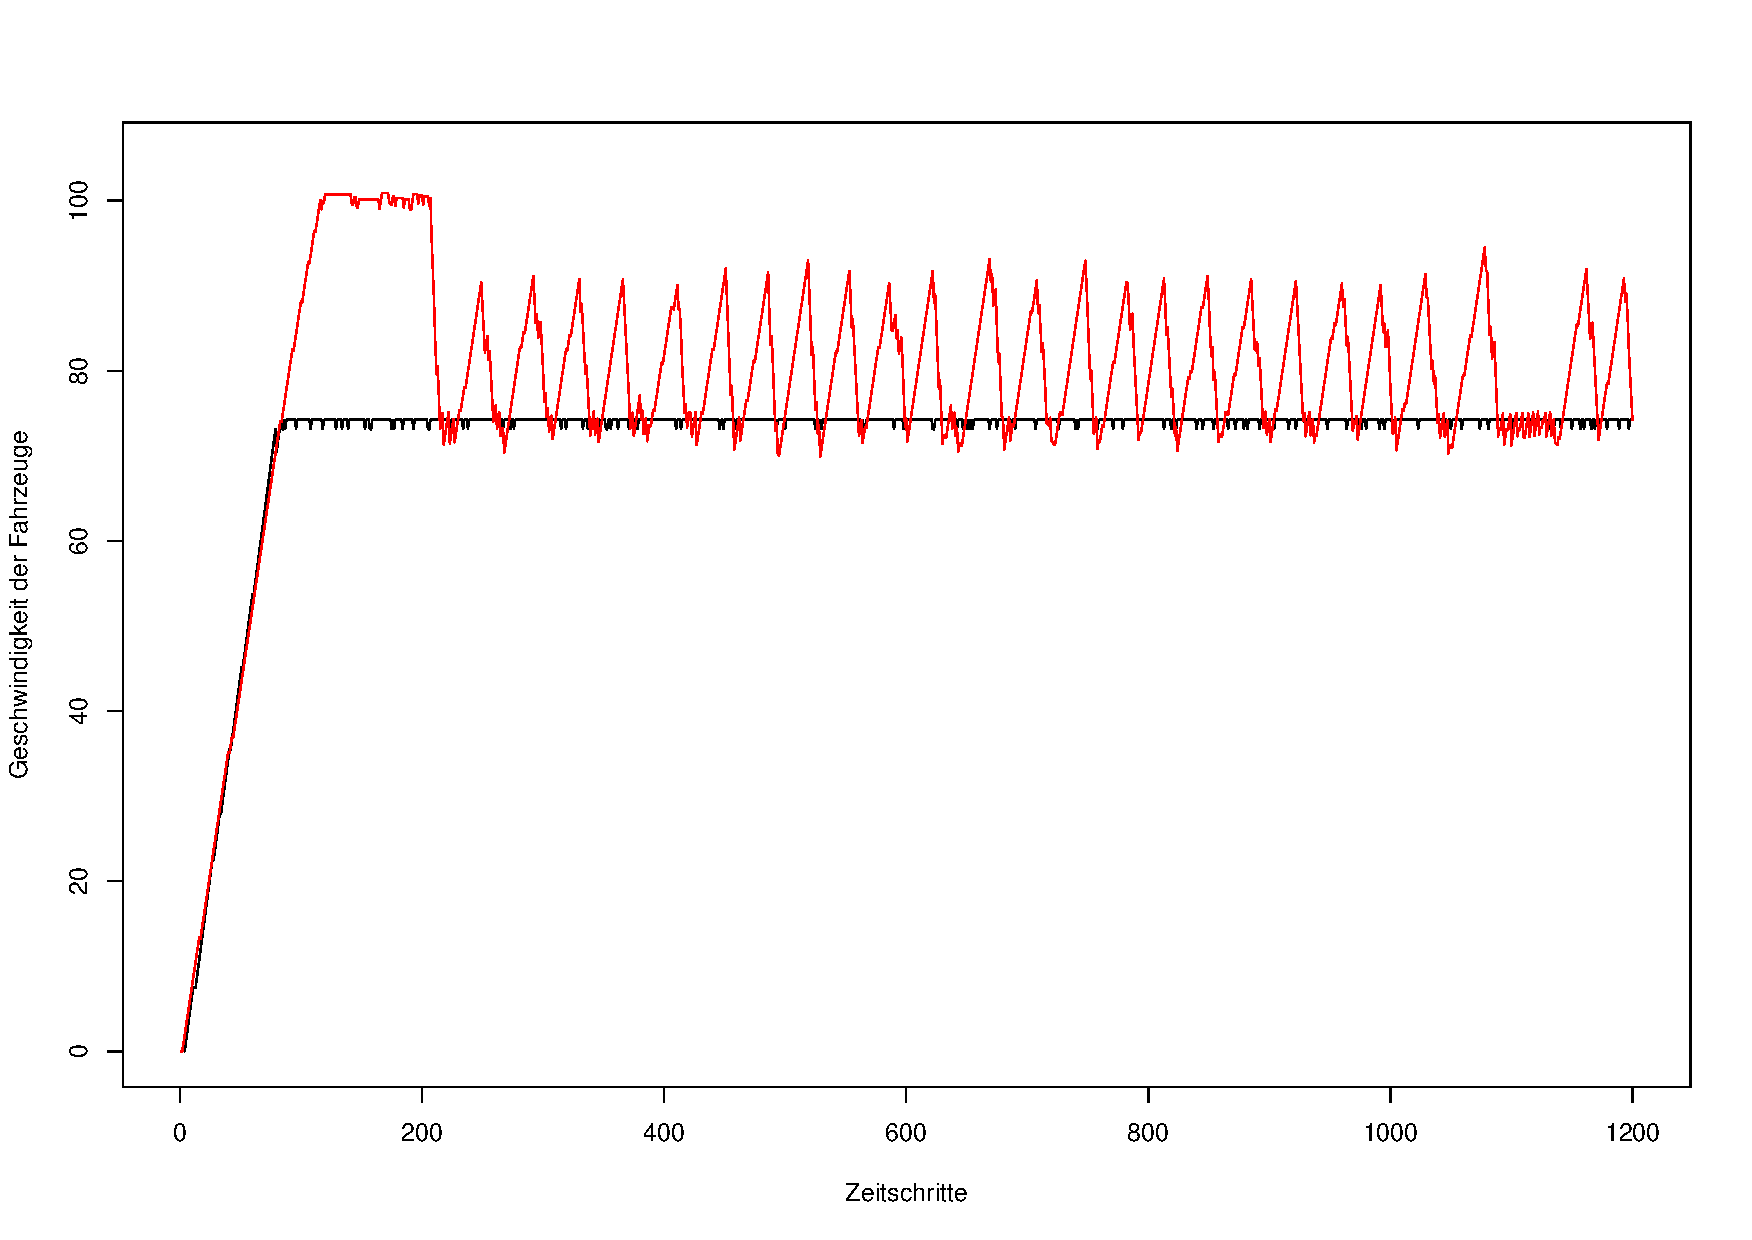
\includegraphics[width=0.3\textwidth]{speed_run7}\label{figure:run7}}\qquad 
   \subfigure[2. Durchlauf]{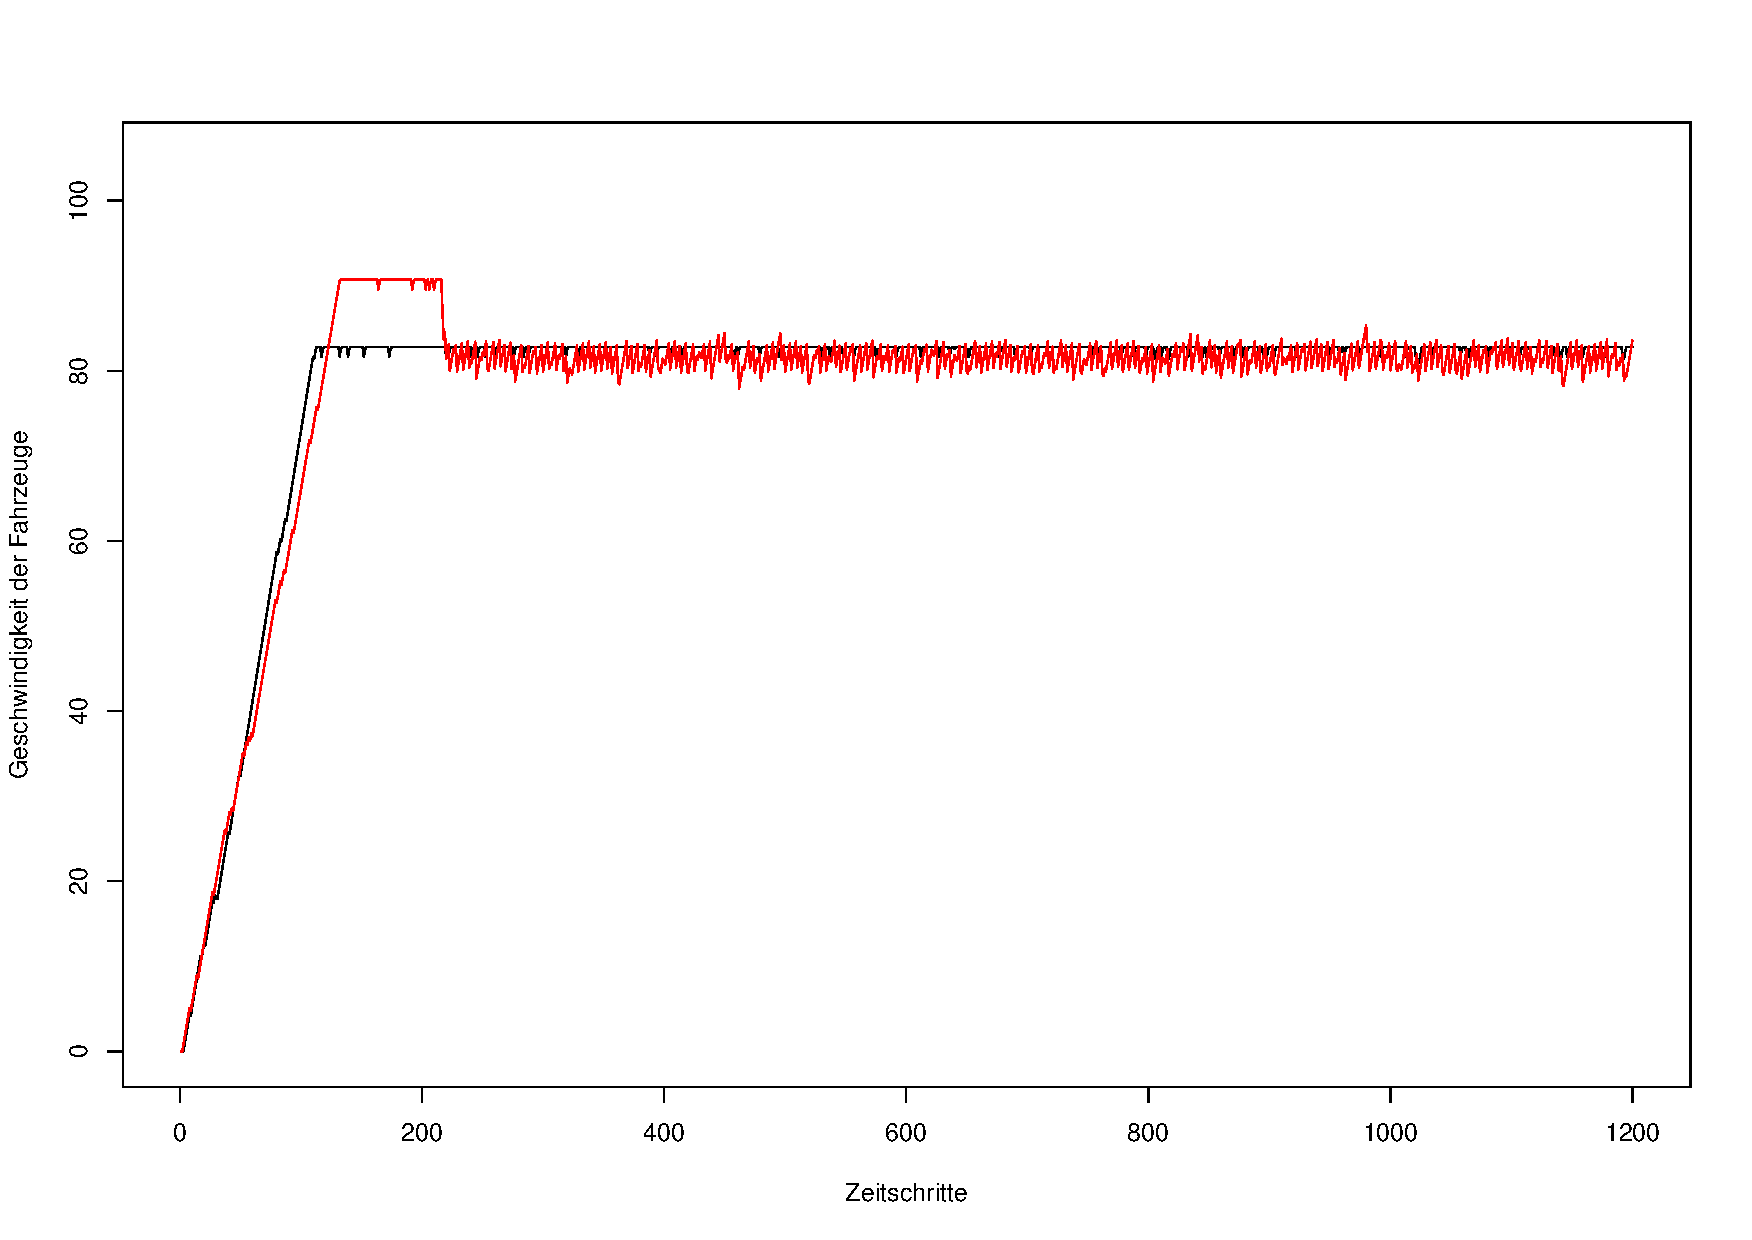
\includegraphics[width=0.3\textwidth]{speed_run8}\label{figure:run8}}\qquad 
   \subfigure[3. Durchlauf]{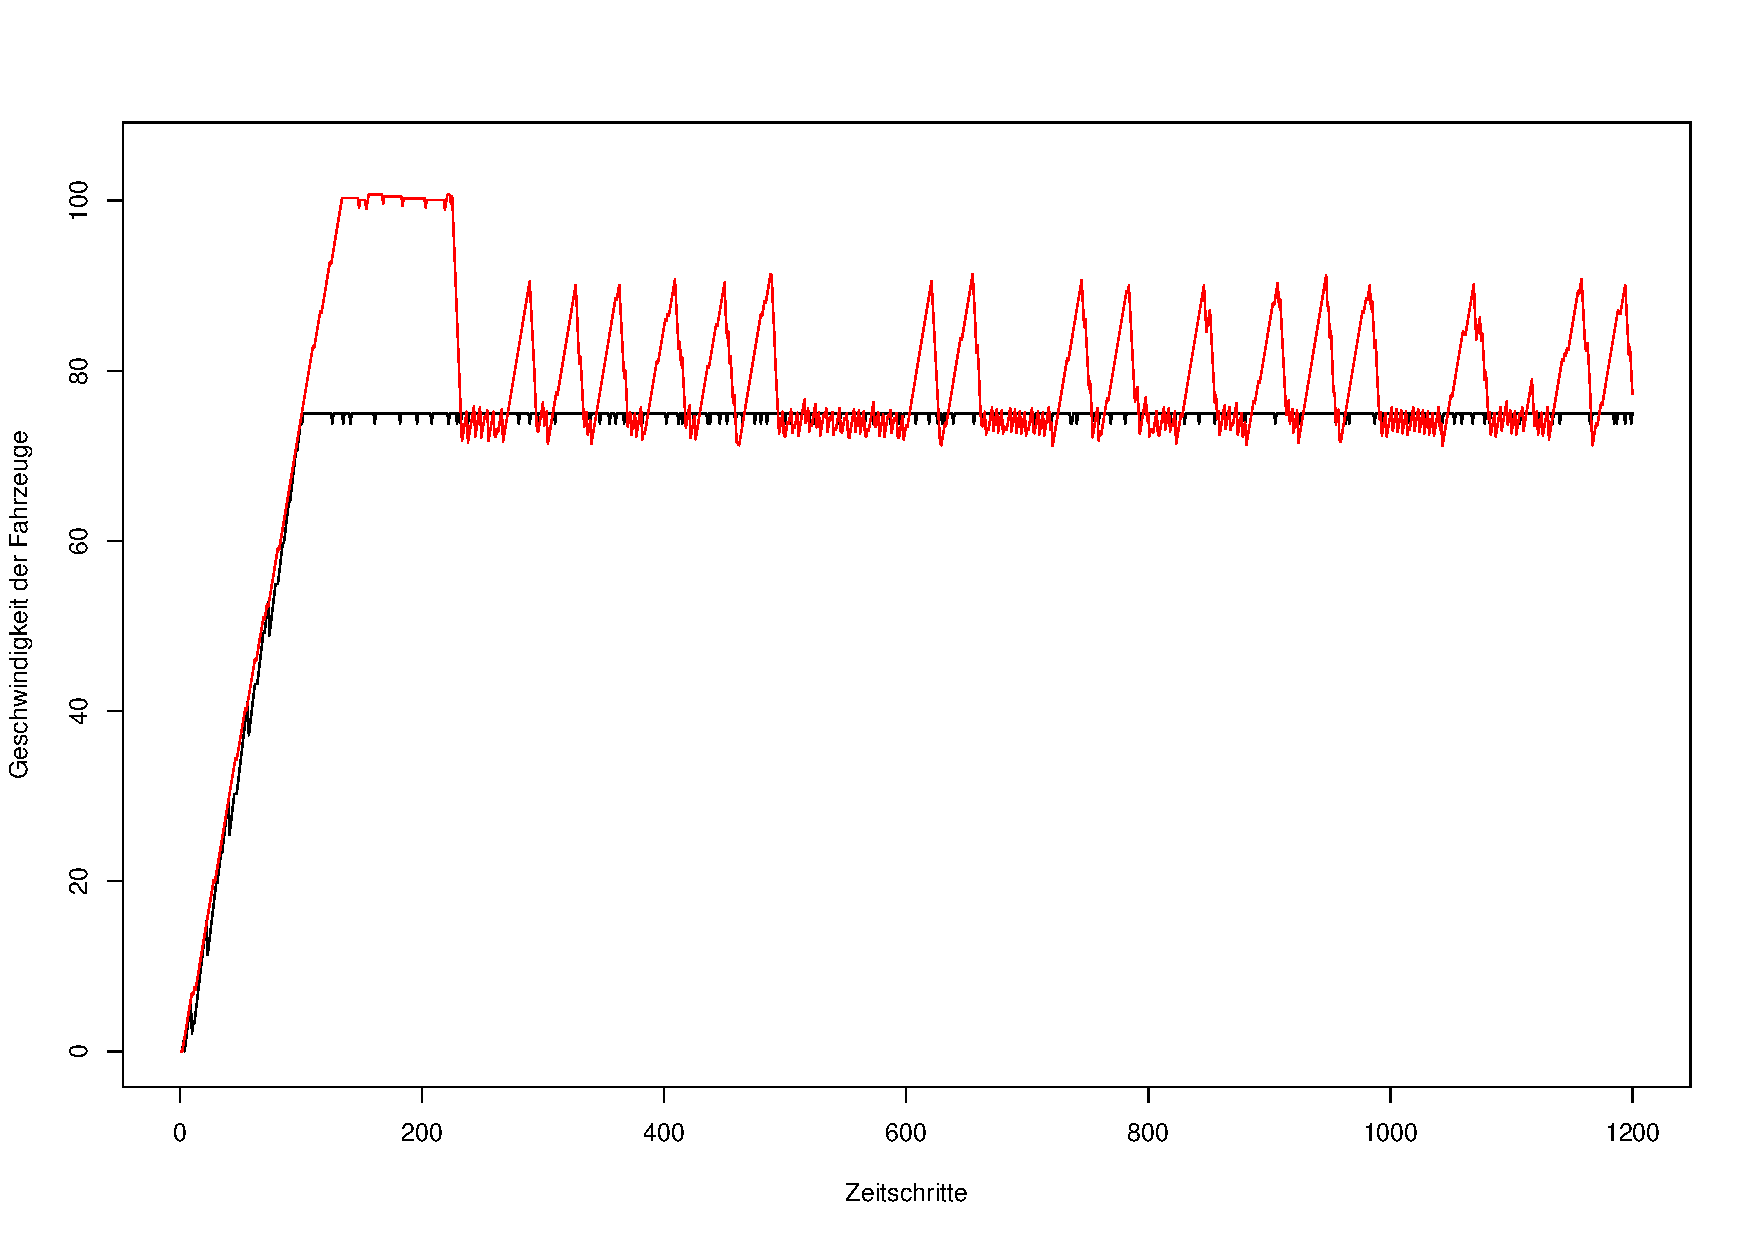
\includegraphics[width=0.3\textwidth]{speed_run9}\label{figure:run9}}
  \caption{Simulationen mit Zellgröße 7,5 m und Zeitschrittlänge 0,025 min} 
  \label{figure:run7-9}
\end{figure}

Die Geschwindigkeitskurve des schnelleren Fahrzeugs weist in \cref{figure:run7} ein sägezahnähnliches Muster auf.
Dies resultiert aus den, im Vergleich zu den herbeigeführten Geschwindigkeitszuwächsen, großen Zellen.
Ein Geschwindigkeitsunterschied von zehn bis 15 km/h reicht bei entsprechend zugrunde liegender Ausgangsgeschwindigkeit nicht aus, eine Verkürzung des Abstands herbeizuführen.
Da sich die Abbrems- und Beschleunigungsmanöver identisch wiederholen, kommt es zu dieser Musterbildung.

Das Plot in \cref{figure:run8} zeigt ein Einordnen hinter dem langsameren Fahrzeug und die Beibehaltung dessen Geschwindigkeit.
Das in \cref{figure:run9} ist nahezu eine Mischform aus den ersten beiden Kurven.


\subsubsection{Zellgröße 5,0 m}

\begin{figure}[hptb]
  \centering 
   \subfigure[1. Durchlauf]{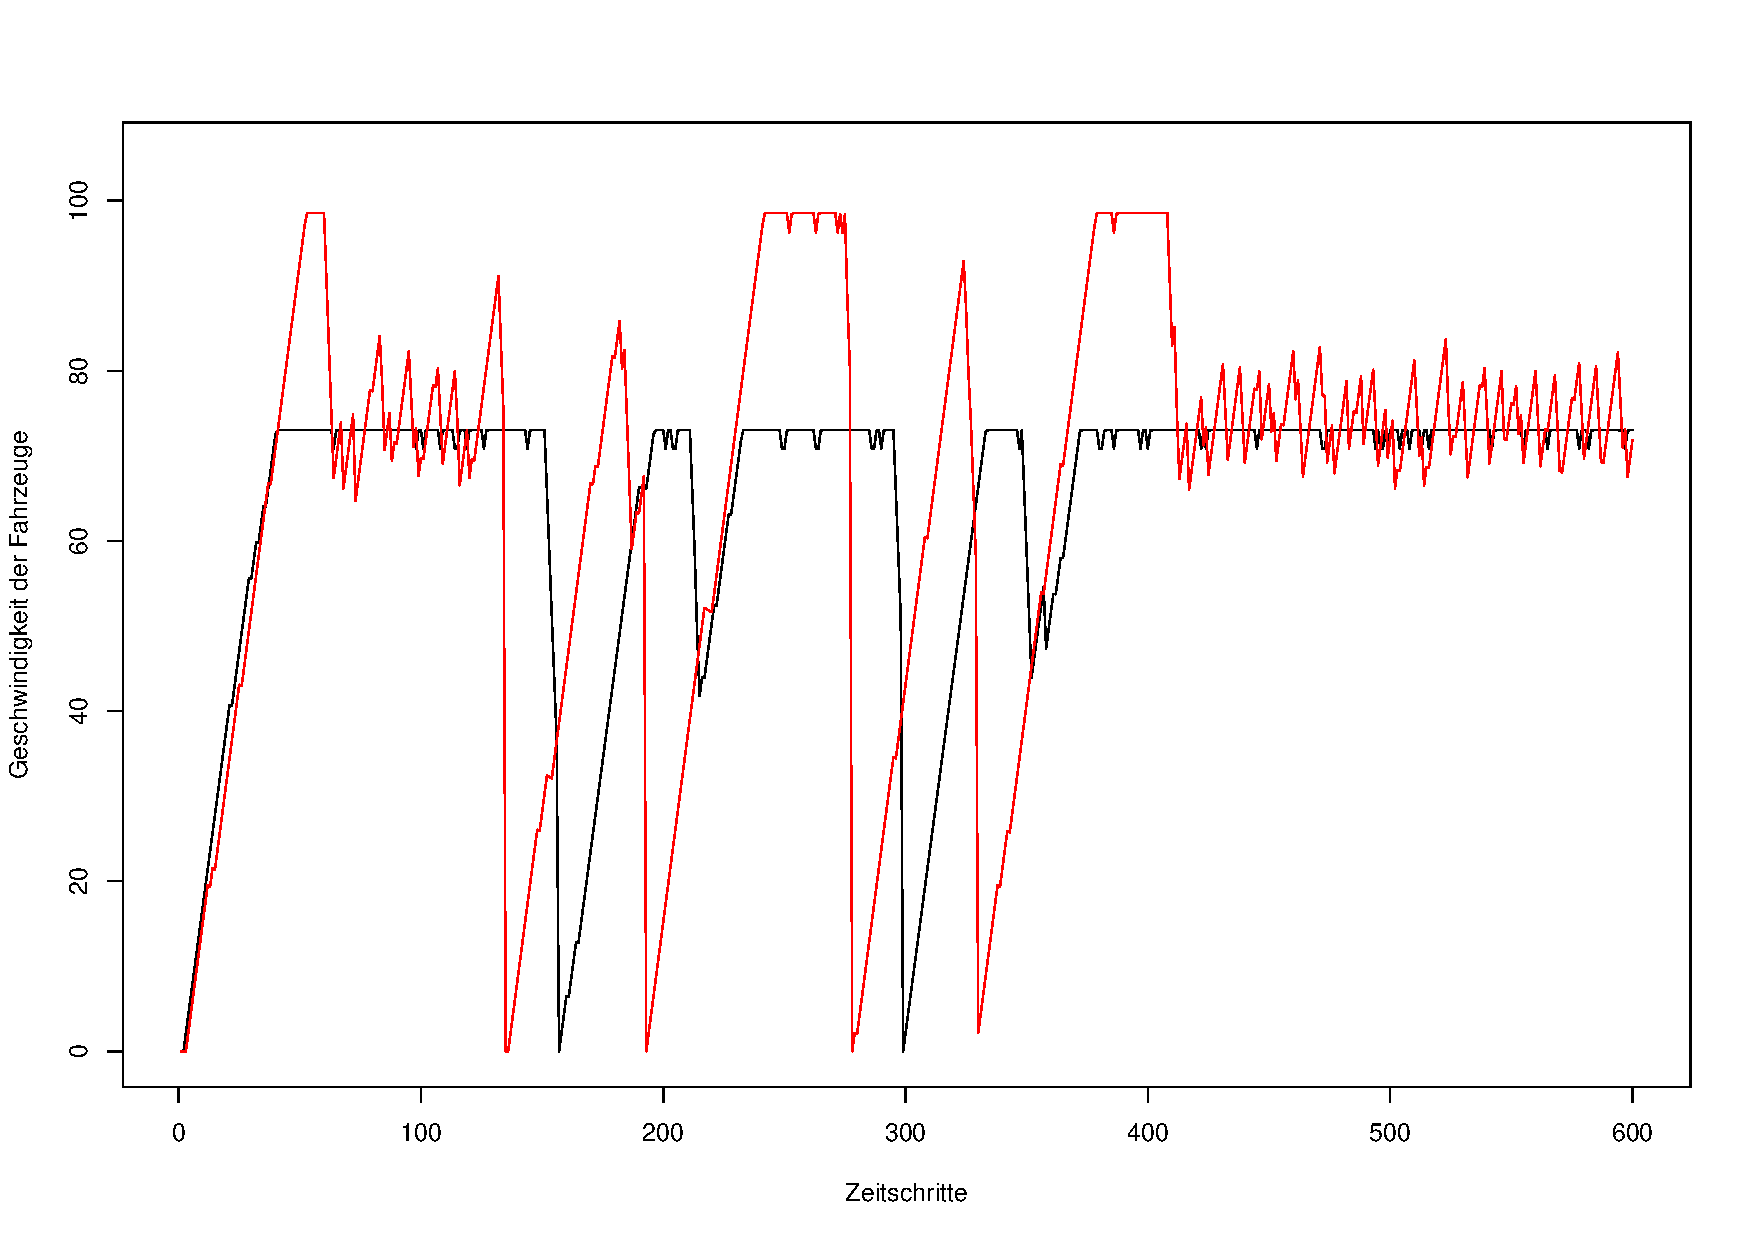
\includegraphics[width=0.3\textwidth]{speed_run14}\label{figure:run14}}\qquad 
   \subfigure[2. Durchlauf]{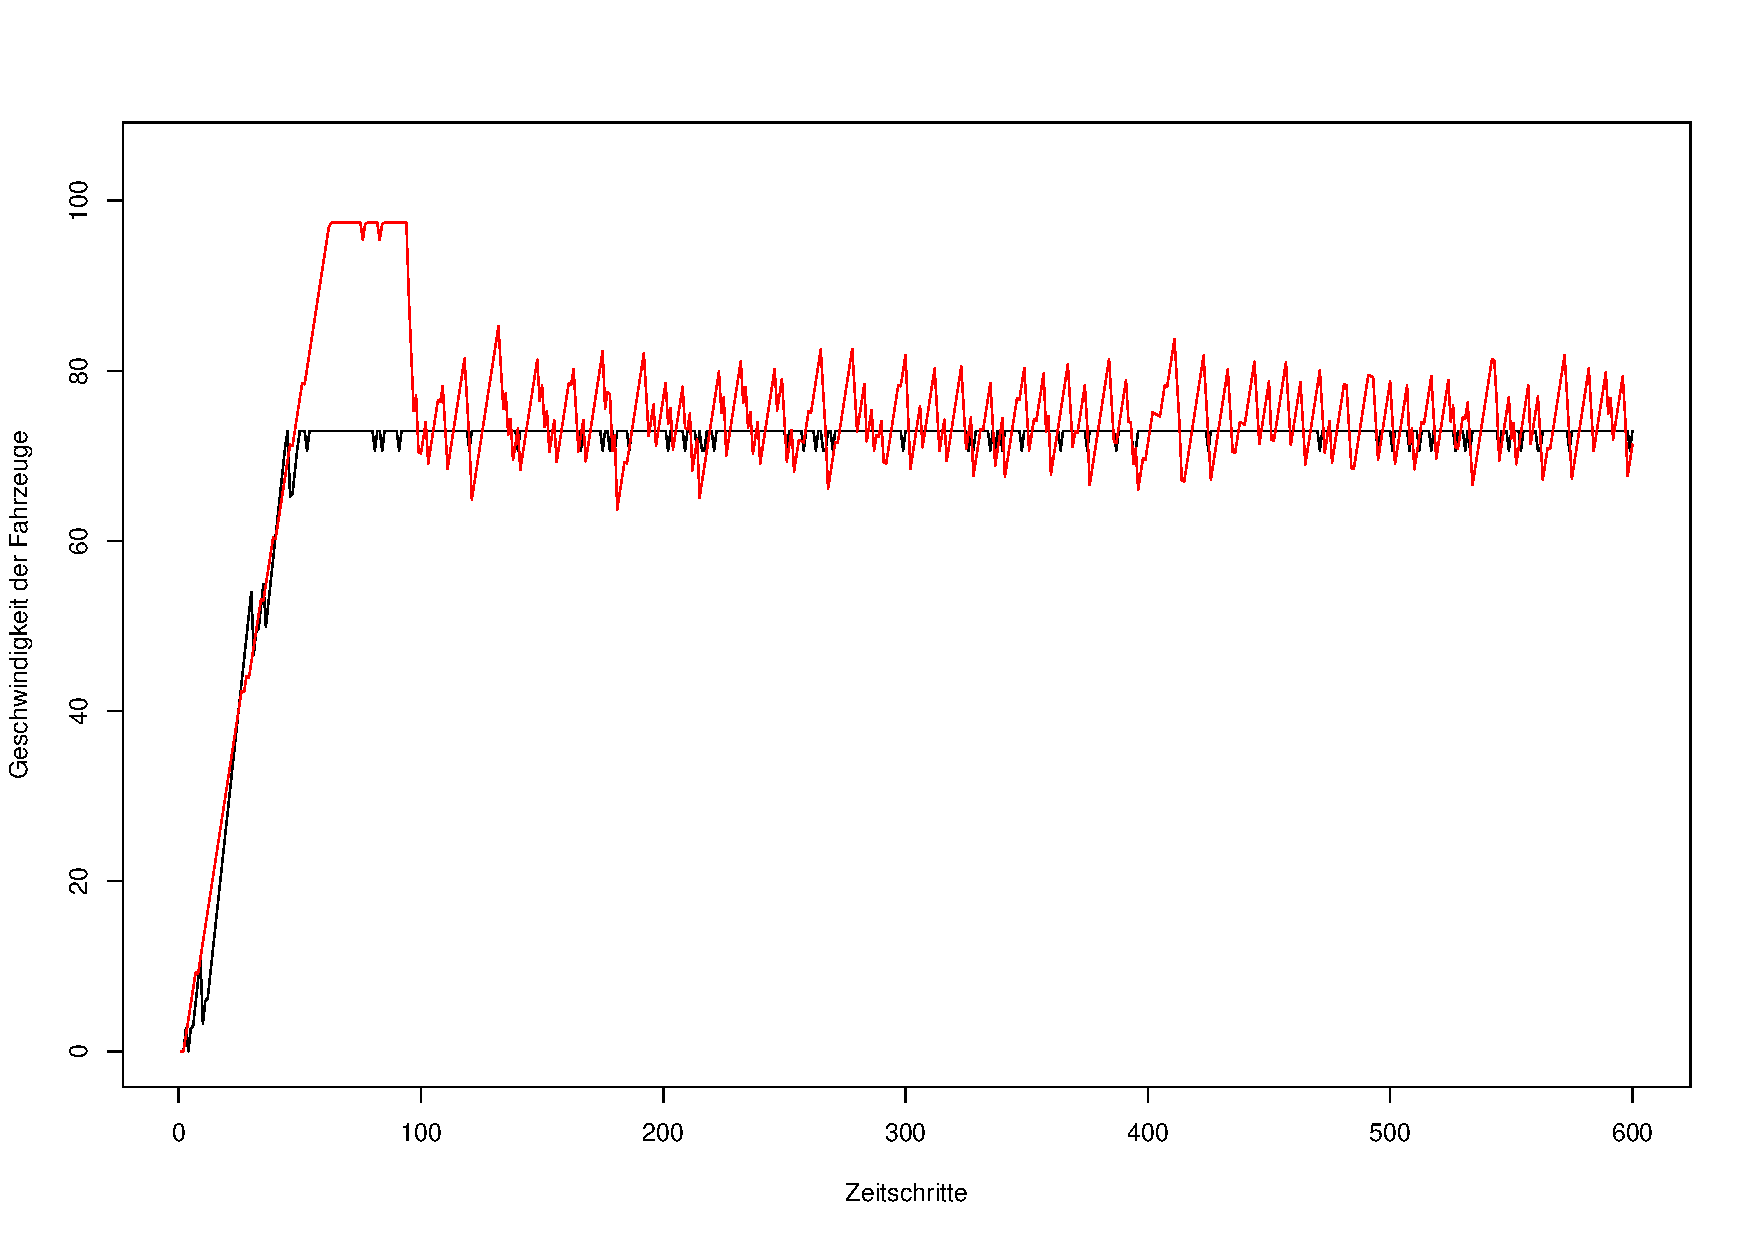
\includegraphics[width=0.3\textwidth]{speed_run15}\label{figure:run15}}\qquad 
   \subfigure[3. Durchlauf]{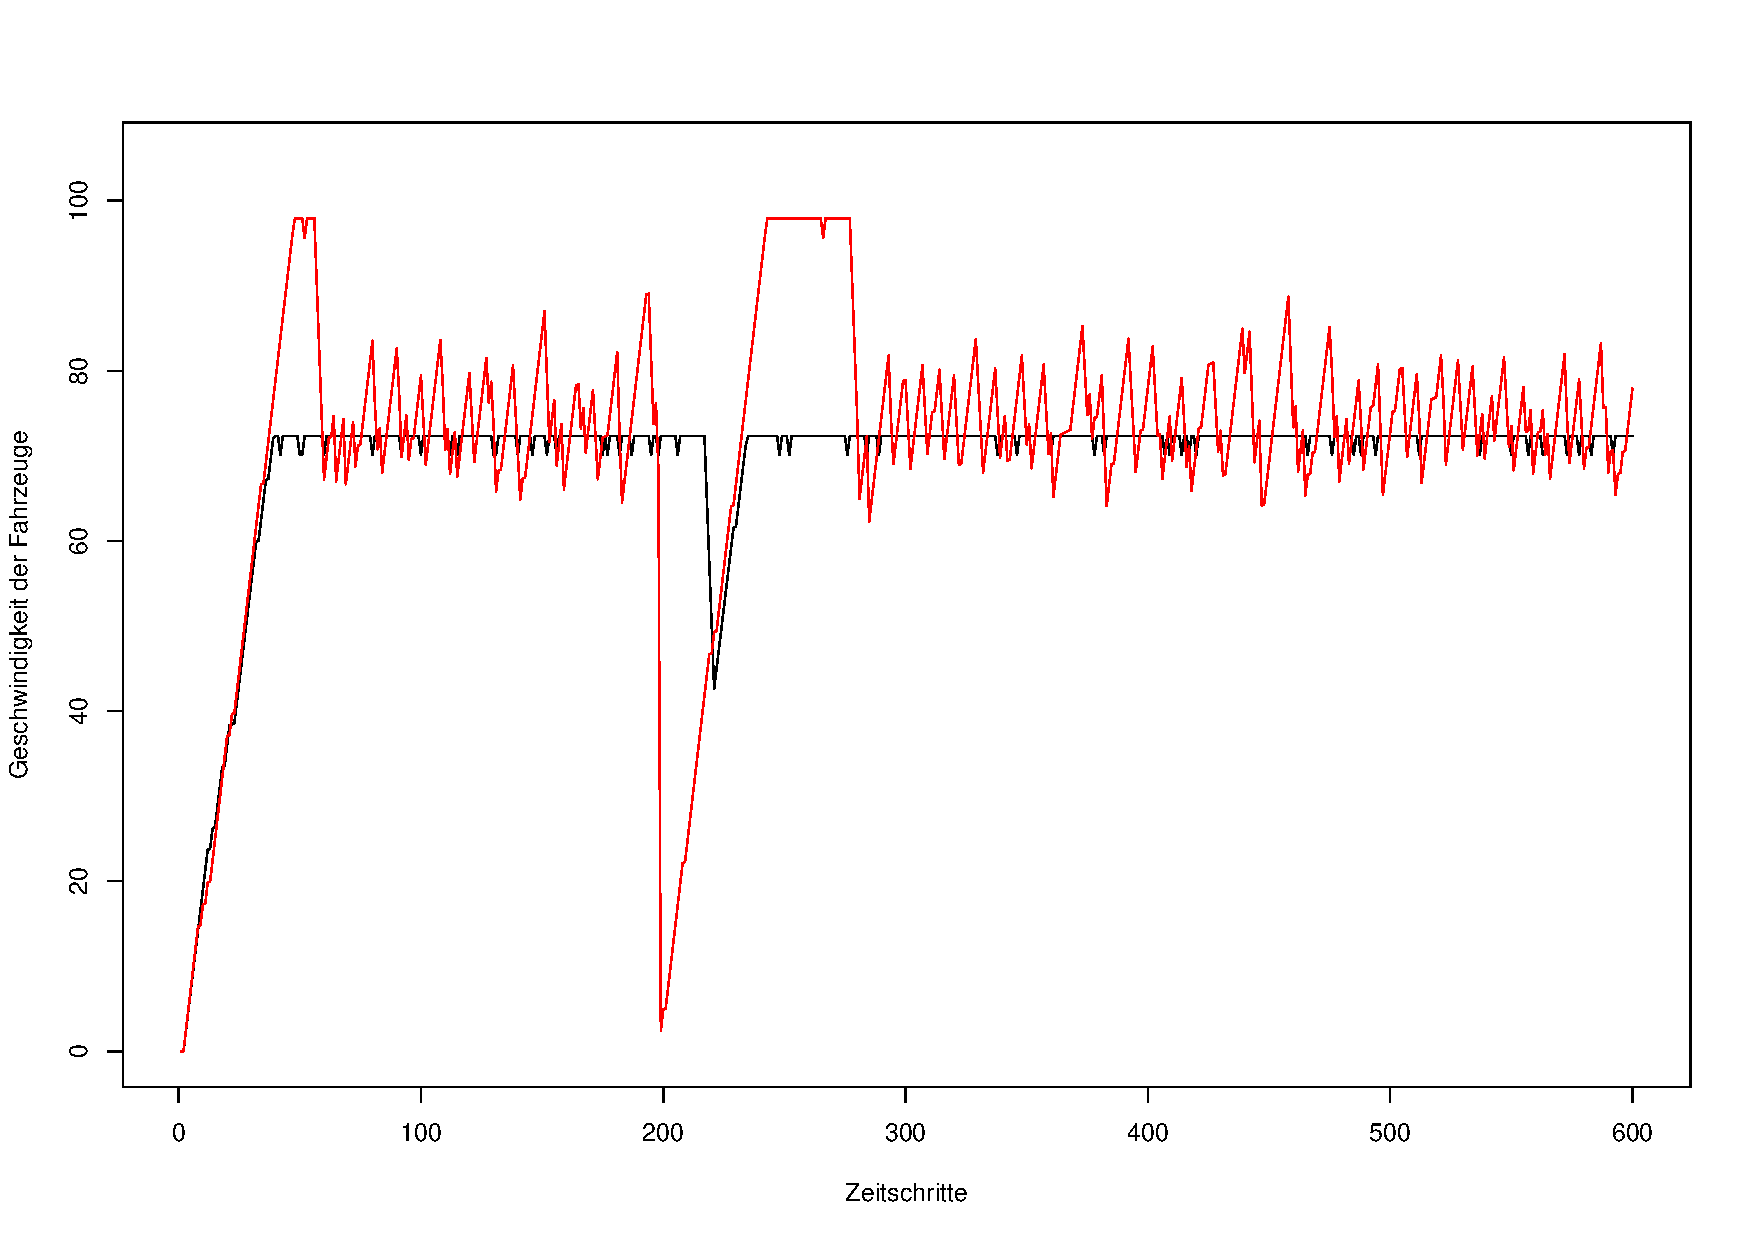
\includegraphics[width=0.3\textwidth]{speed_run16}\label{figure:run16}}
  \caption{Simulationen mit Zellgröße 5,0 m und Zeitschrittlänge 0,05 min} 
  \label{figure:run14-16}
\end{figure}

Die Diagramme in \cref{figure:run14-16} zeigen wiederholt, dass der Abstand, der für den Bremsvorgang zur Verfügung steht, mit einem recht langen Zeitraum zwischen den Zeitschritten, nicht ausreicht.

Allerdings ist im ersten und im dritten Durchlauf zu erkennen, dass das langsamere Fahrzeug, ohne dass es zu einer Kollision kommen muss, für das gerade beschleunigende Fahrzeug abbremsen konnte. 

\begin{figure}[hptb]
  \centering 
   \subfigure[1. Durchlauf]{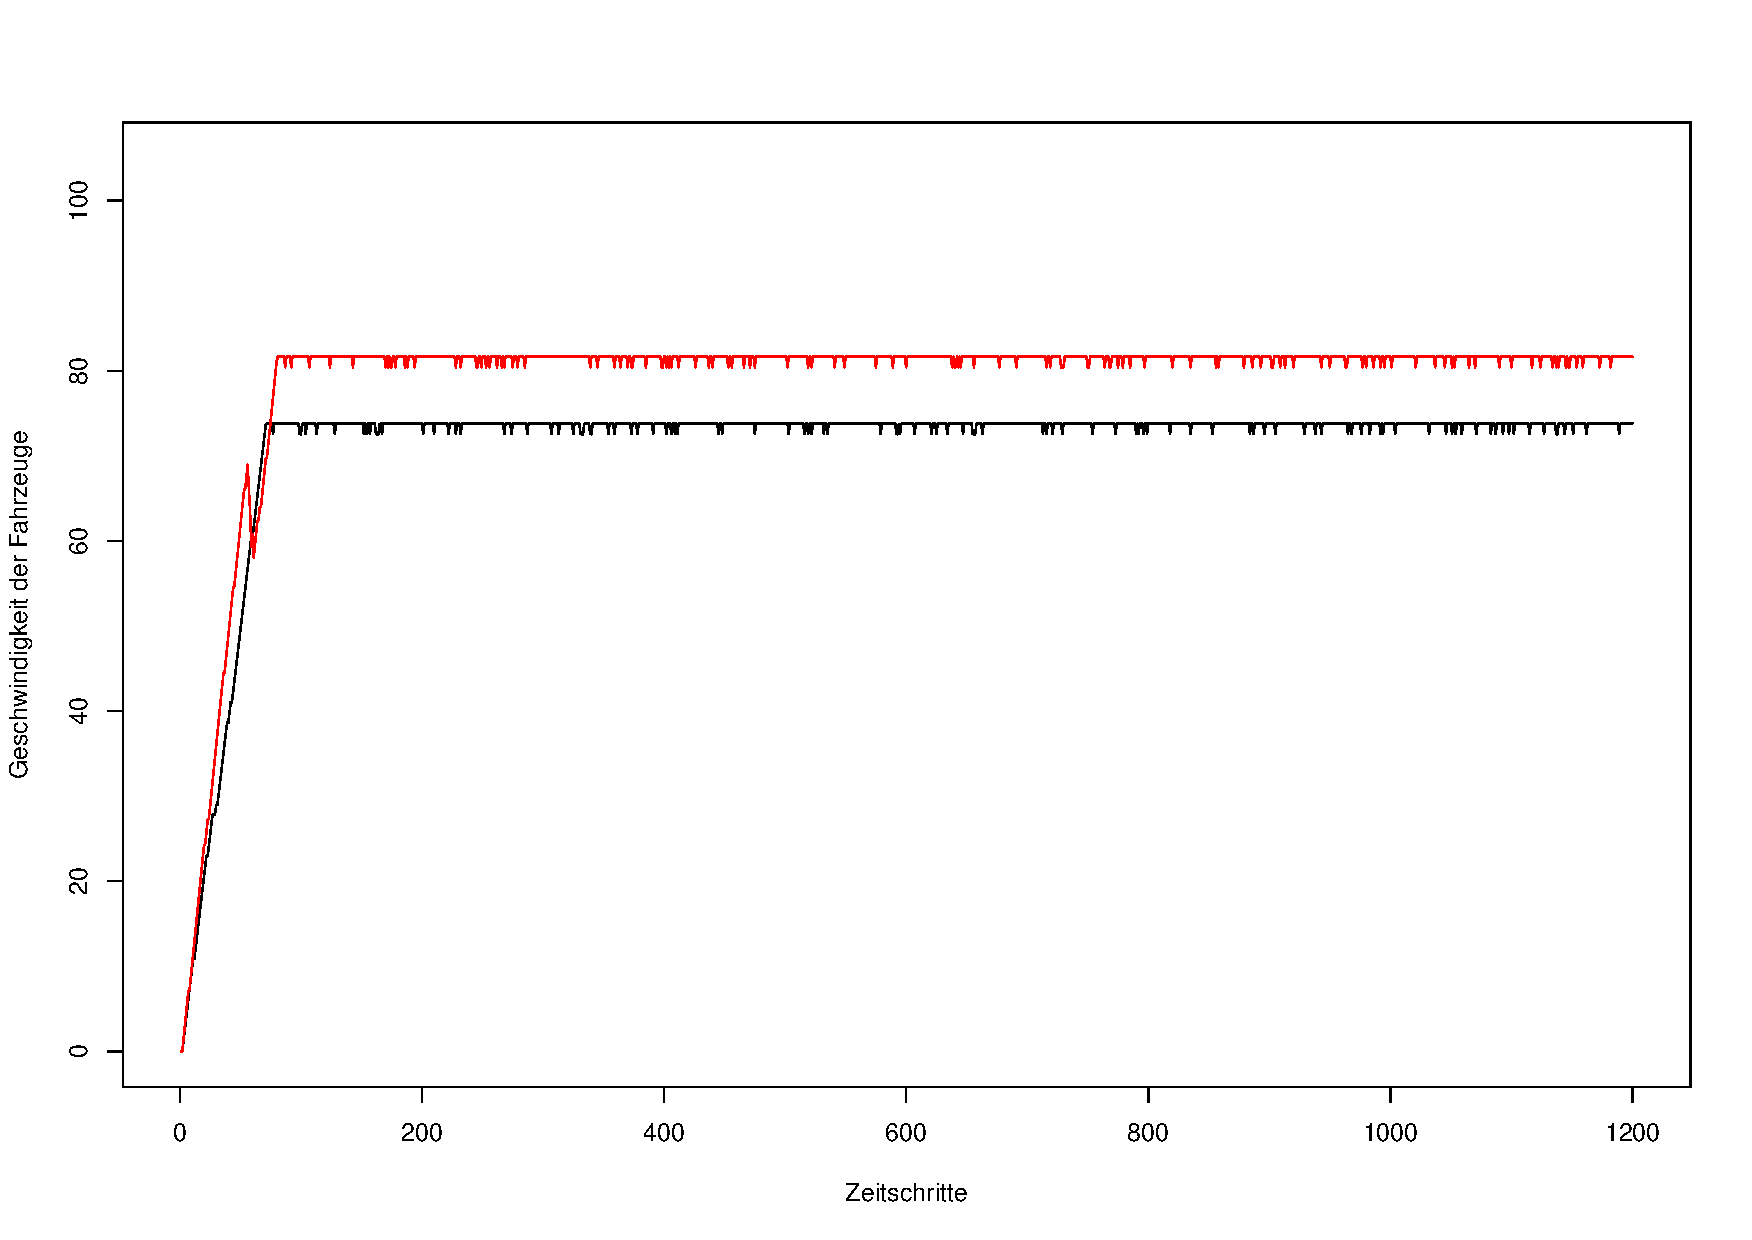
\includegraphics[width=0.3\textwidth]{speed_run17}\label{figure:run17}}\qquad 
   \subfigure[2. Durchlauf]{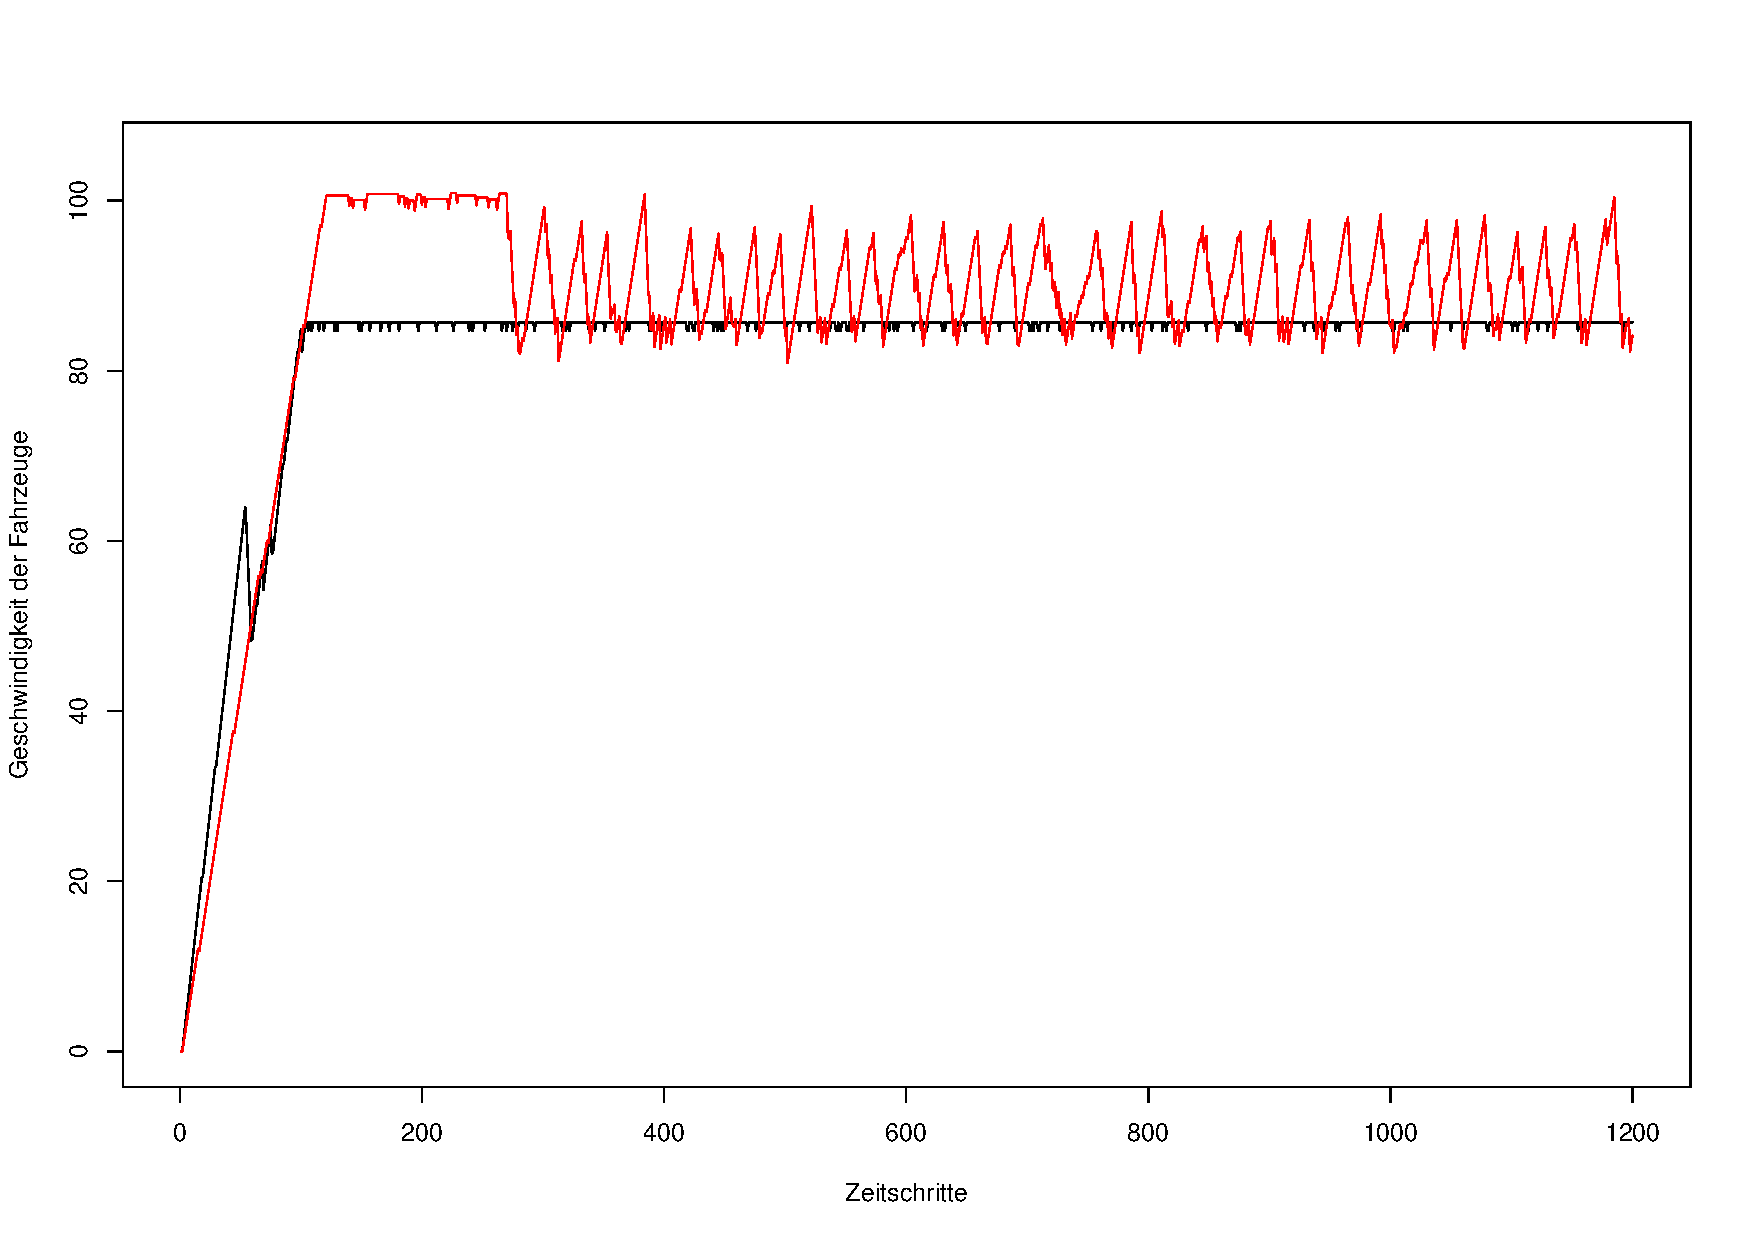
\includegraphics[width=0.3\textwidth]{speed_run18}\label{figure:run18}}\qquad 
   \subfigure[3. Durchlauf]{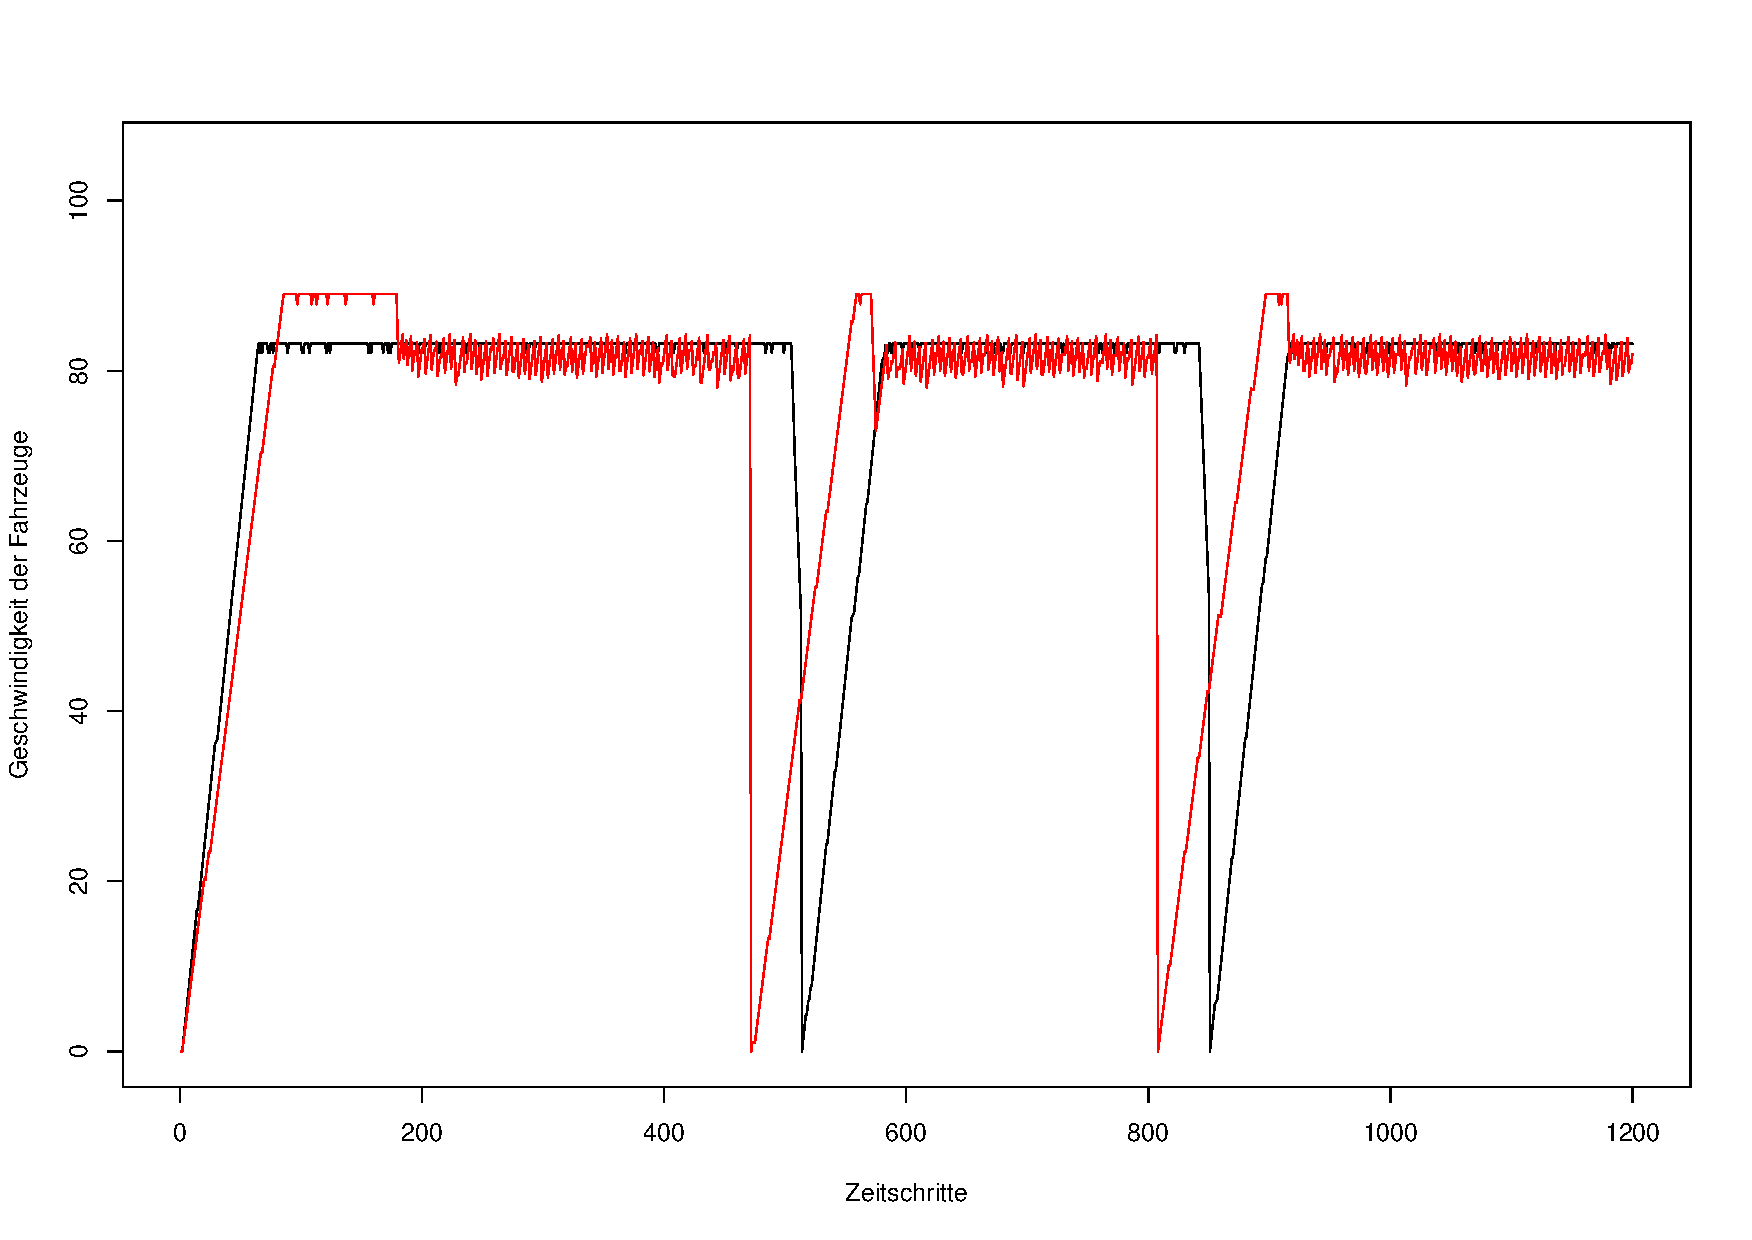
\includegraphics[width=0.3\textwidth]{speed_run19}\label{figure:run19}}
  \caption{Simulationen mit Zellgröße 5,0 m und Zeitschrittlänge 0,025 min} 
  \label{figure:run17-19}
\end{figure}

Die drei Durchläufe mit einer Zeitschrittlänge von 0,025 min ergaben ein uneinheitliches Bild.
In \cref{figure:run17} konnte das schnellere Fahrzeug wieder mit höherer Geschwindigkeit hinter dem langsameren herfahren, scheinbar ohne dass ein Raumgewinn passierte, der zu einer Verzögerung geführt hätte.
\\
Evtl. fuhr das schnellere Fahrzeug auch mit seiner max. möglichen Geschwindigkeit und der Geschwindigkeitsunterschied war so gering, das es in der Simulationszeit das langsamere Fahrzeug nicht erreichte.

Der Durchlauf im Diagramm in \cref{figure:run18} zeigt wieder das sägezahnähnliche Muster, wie es mit den größeren Zelldimensionen bereits der Fall war.

Unerwarteterweise kam es im dritten Durchlauf zu je zwei Kollisionen.
Besonders die jeweils auslösende Kollision des ursprünglich schnelleren Fahrzeuges war nicht zu erklären, da der Geschwindigkeitsunterschied in beiden Fällen minimal gewesen war.

Ein weiterer Durchlauf, siehe \cref{figure:run19a}, der einen vergleichbaren Ablauf hervorbrachte, bei dem aber die Ausgabe der Fahrzeugdaten im Kontrollfenster erfolgte, konnte das Verhalten aufklären.
Die Bedingung im Agentenplan waren so formuliert, dass das Folgefahrzeug dem vorausfahrenden folgen konnte, ohne dass ein \enquote{Sicherheitsabstand} gebildet wurde, wenn die Geschwindigkeit jenes Fahrzeuges nicht größer als die des vorausfahrenden Fahrzeuges war. 
\\
Somit genügte, gewisse Geschwindigkeiten vorrausgesetzt, eine kleine Beschleunigung, um im nachfolgenden Zeitschritt die für die Geschwindigkeit erforderliche Wegstrecke nicht mehr umsetzen zu können.

\begin{figure}[hptb]
  \centering 
   \subfigure[ursprüngliches Verhalten]{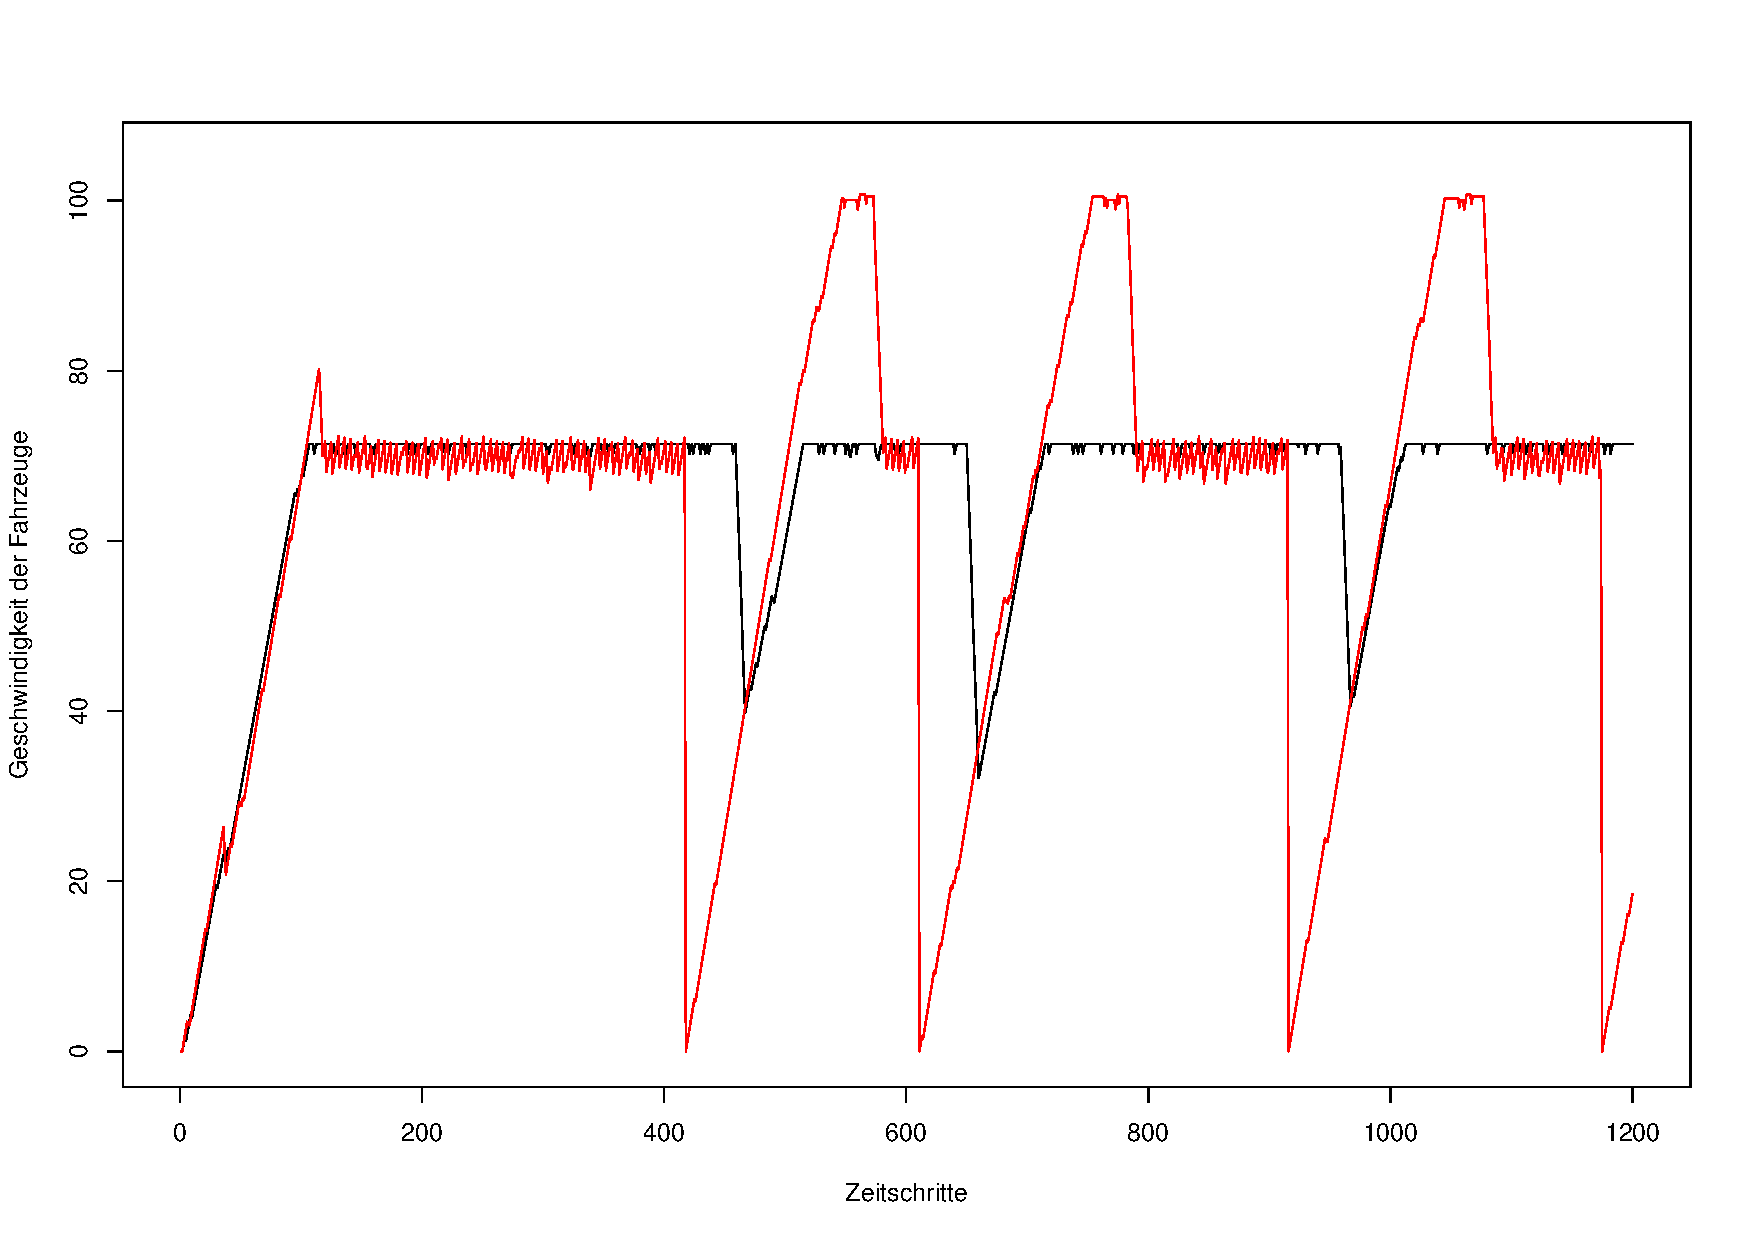
\includegraphics[width=0.3\textwidth]{speed_run19a}\label{figure:run19a}}\qquad 
   \subfigure[Modifikation 1]{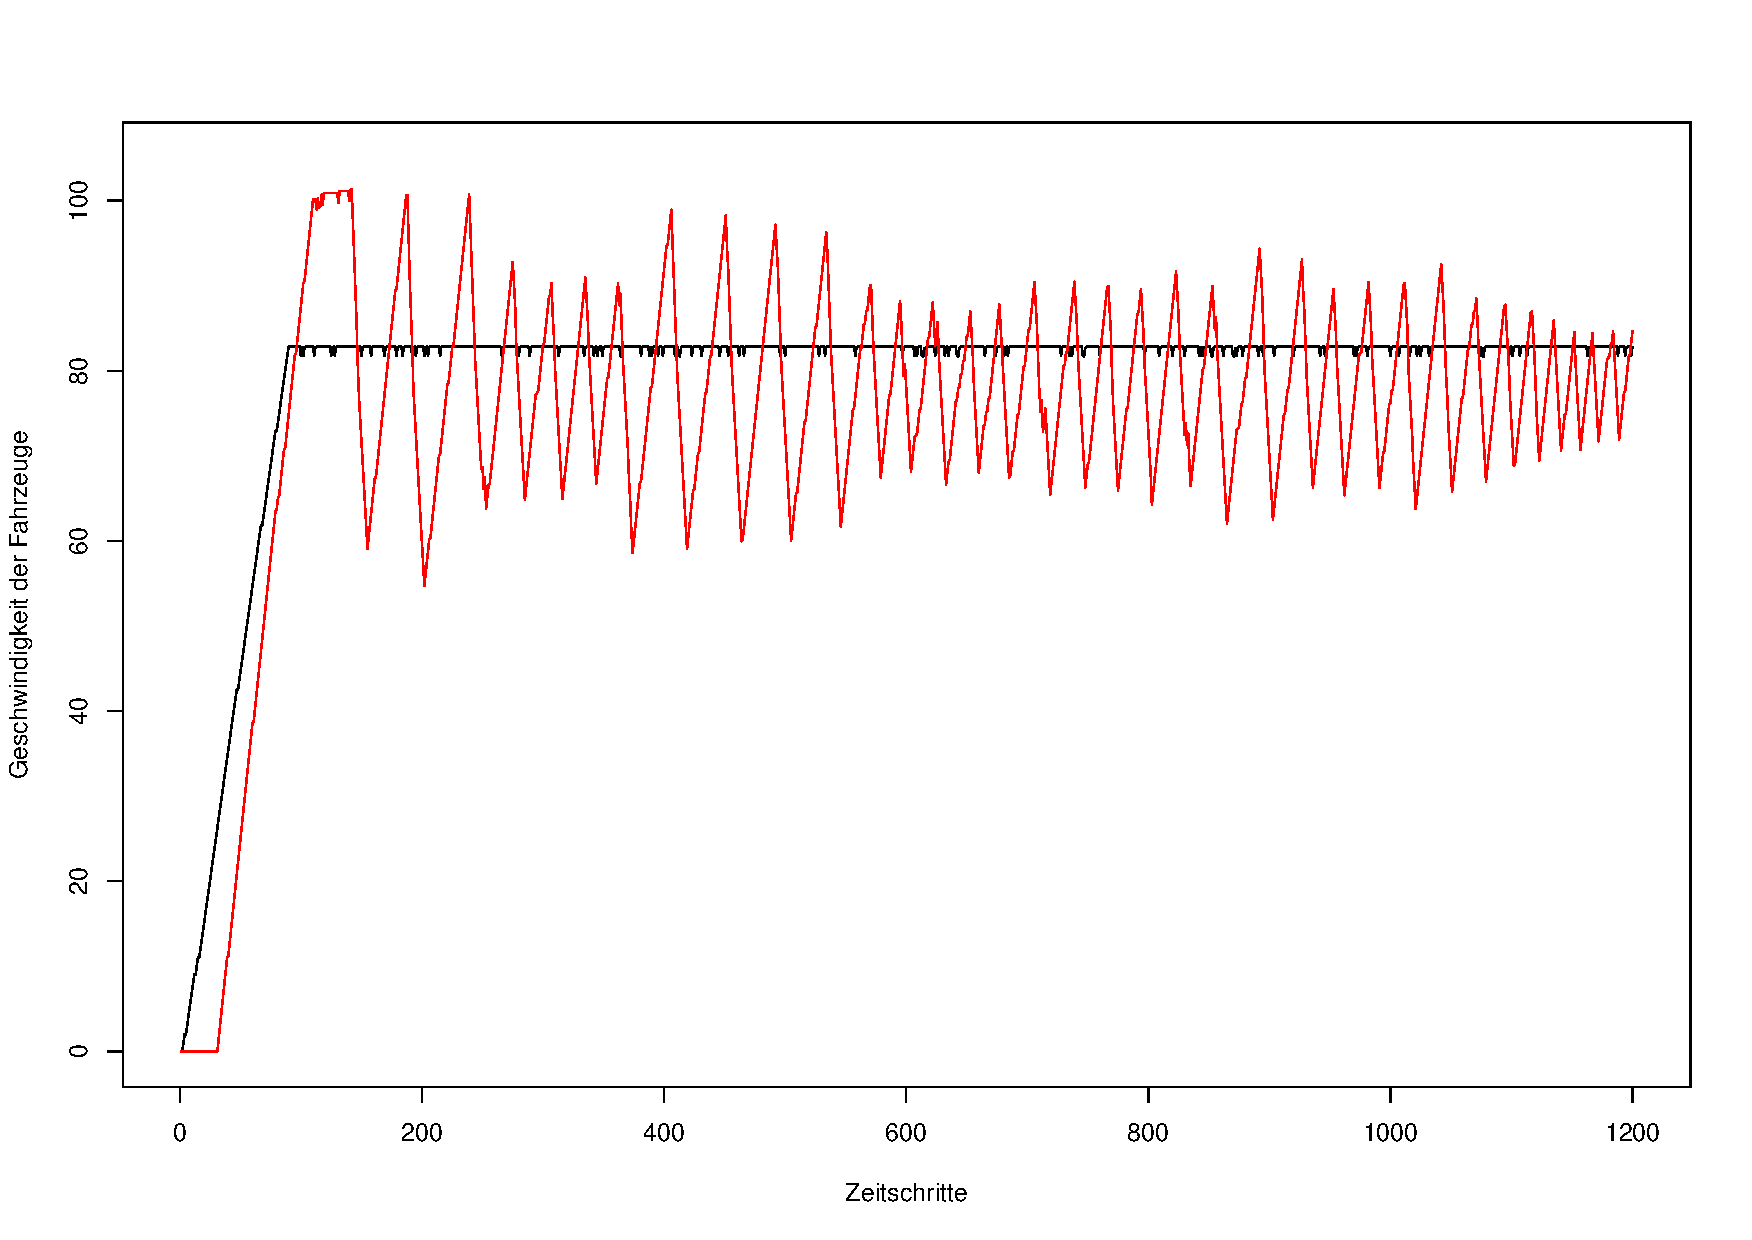
\includegraphics[width=0.3\textwidth]{speed_run19b}\label{figure:run19b}}\qquad 
   \subfigure[Modifikation 2]{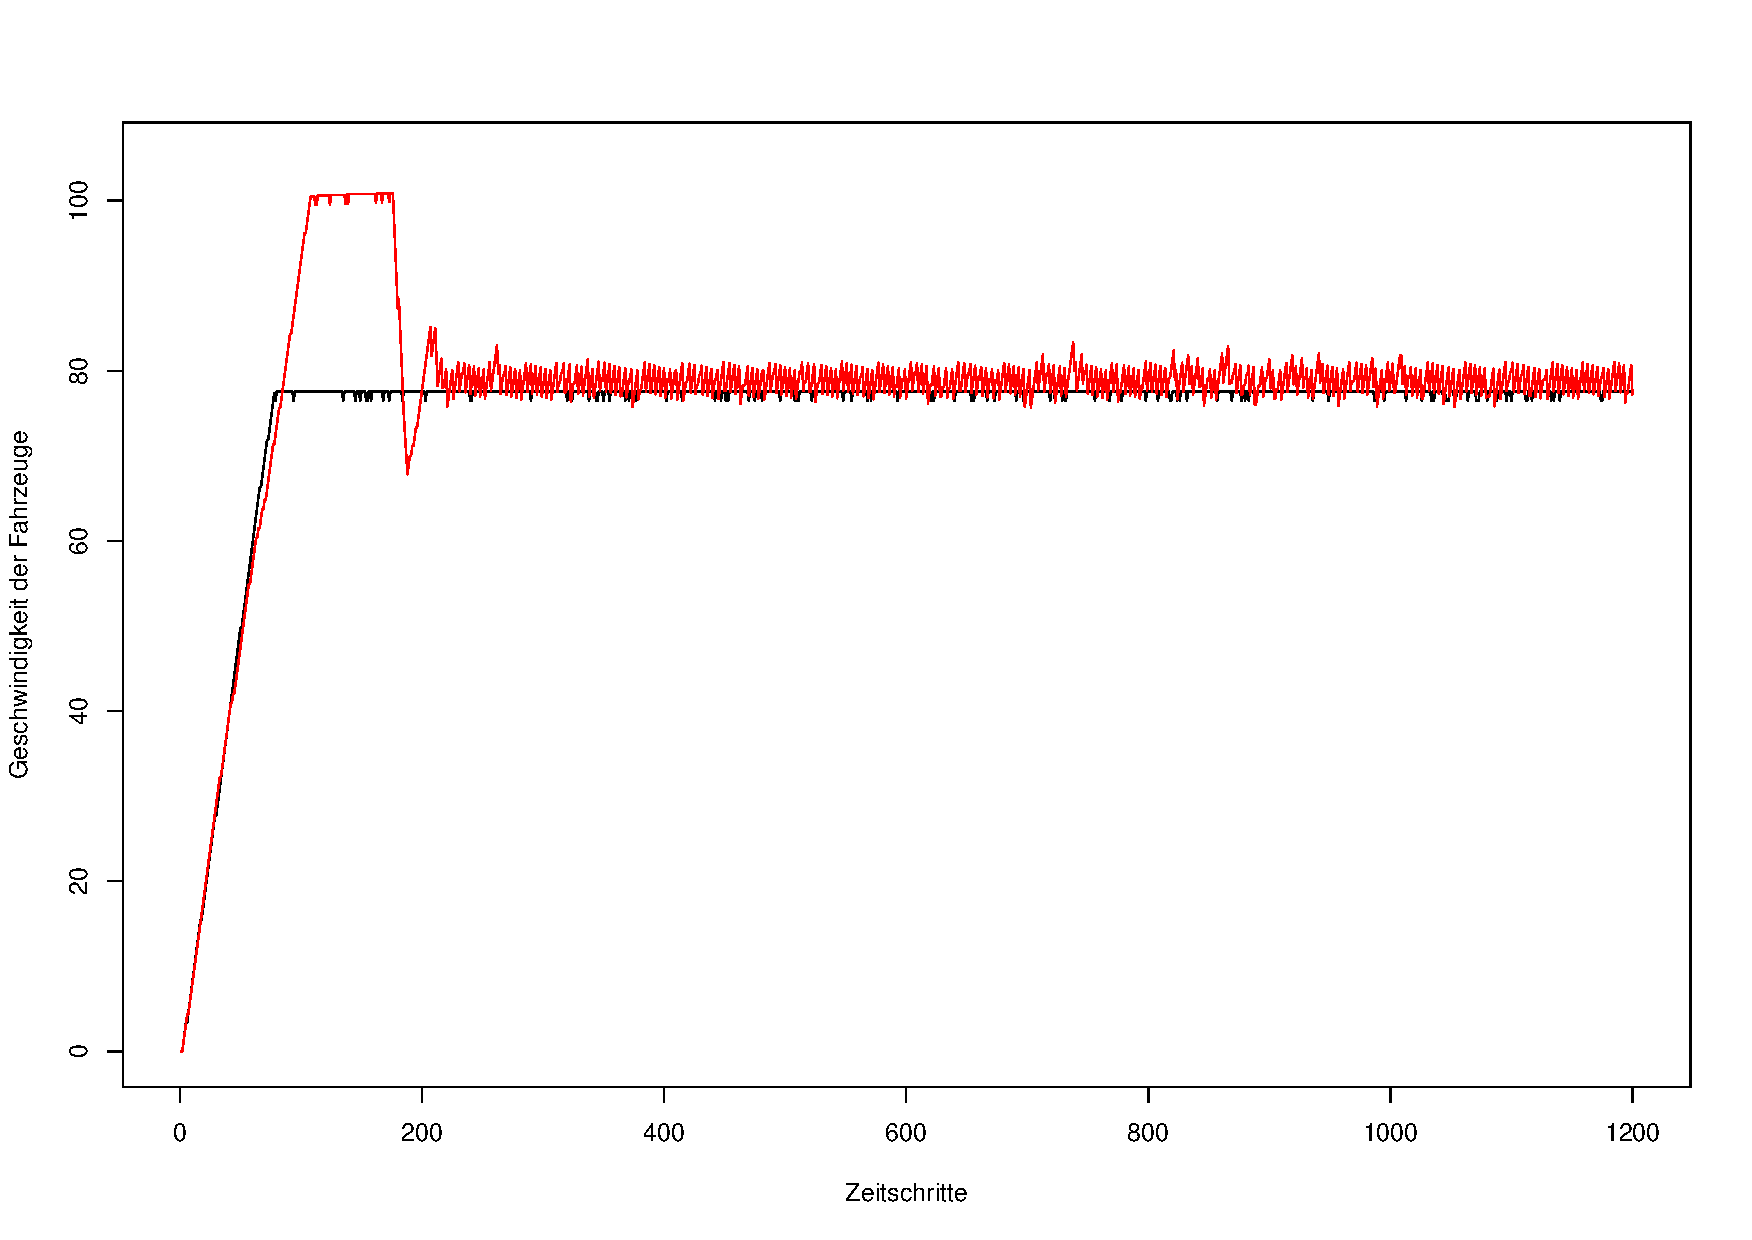
\includegraphics[width=0.3\textwidth]{speed_run19c}\label{figure:run19c}}
  \caption{Simulationen mit Veränderungen in den Agentenplänen} 
  \label{figure:run19a-c}
\end{figure}

Eine erste Modifikation führte wieder zurück zu einem Verhalten, siehe \cref{figure:run19b}, aufgrund dessen die Geschwindigkeitskomponente mit in die Verzögerungslogik eingefügt worden war. 
\\
Das nachfolgende Fahrzeug bremste so lange ab, bis der gewünschte Abstand erreicht war, um daraufhin mit einem \enquote{Zwischensprint} wieder auf das vorausfahrende Fahrzeug aufzuschließen.
Durch den Geschwindigkeitsüberschuss, der abgebaut werden muss, wurde der Abstand wieder extrem verkürzt, dass der Kreislauf von vorn beginnt.
\\
In einigen Simulationsläufen musste die Geschwindigkeit derart massiv abgebaut werden, dass das Folgefahrzeug fast zum Stillstand kam.

Es musste ein Weg gefunden werden, die Geschwindigkeit von \enquote{Ego} in Zusammenhang mit der Entfernung vom vorausfahrenden Fahrzeug zu bringen.
\\
Verschiedene Ansätze, bei denen in den Bedingungen der Logik mit den vorliegenden Werten Berechnungen durchzuführen gewesen wären, wurden von der Simulationsplattform nicht unterstützt.
\\
Da den Agenten sowohl die eigene Geschwindigkeit als auch die Entfernung als numerische Werte bekannt sind, werden diese nun zu einander in Beziehung gesetzt.

Dies führt dazu, dass die eigene Geschwindigkeit des betrachteten Fahrzeugs gleichzeitig der jeweilige Mindestabstand vom Vordermann sein muss. 
\\
Eine gleichwertige Bedingung wurde auch für die Simulation der Beschleunigung übernommen.
Der reine Geschwindigkeitsvergleich wurde entfernt.


\subsubsection{Zellgröße 2,5 m}

Aufgrund der Veränderung in den Agentenplänen wurde die erneut verringerte Zellgröße ebenfalls mit den beiden verbliebenen Zeitschrittwerten simuliert.

\begin{figure}[hptb]
  \centering 
   \subfigure[1. Durchlauf]{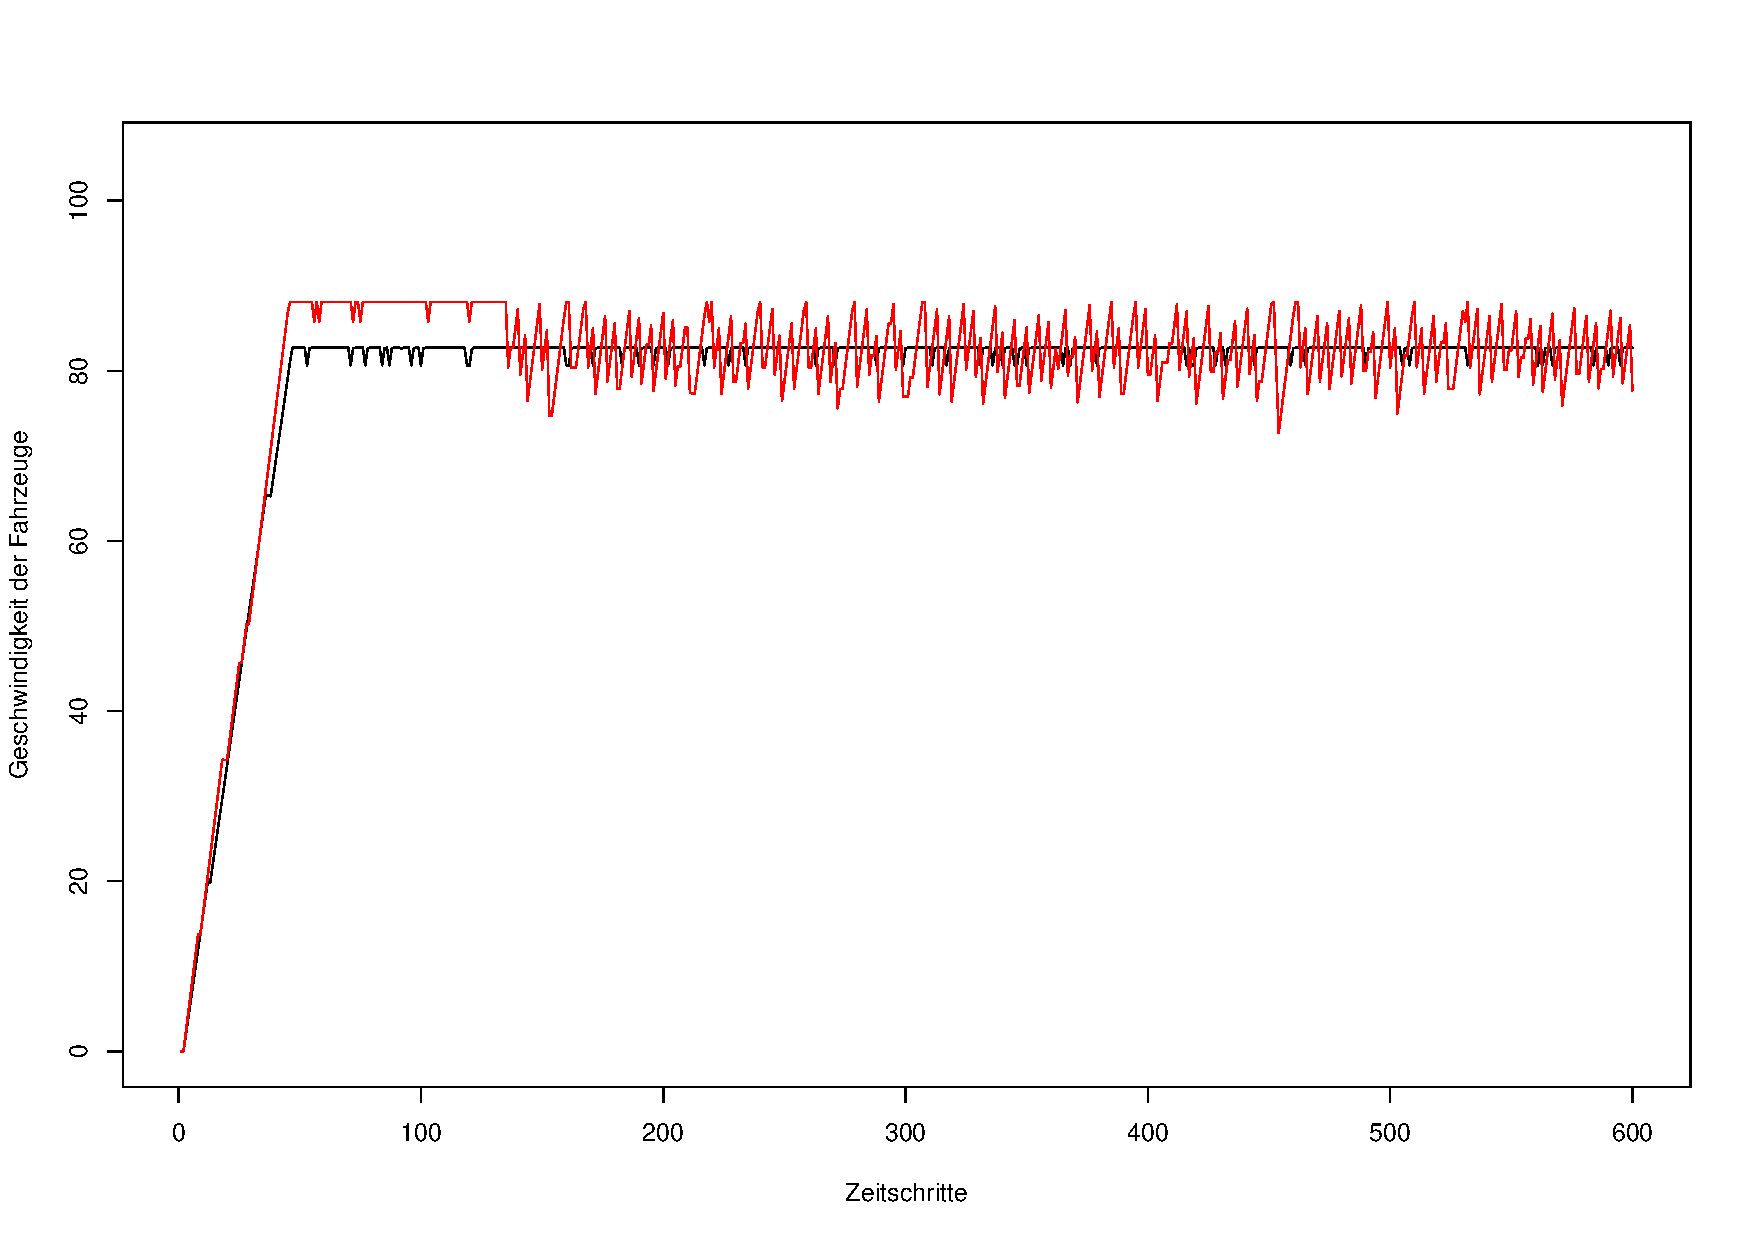
\includegraphics[width=0.3\textwidth]{speed_run24}\label{figure:run24}}\qquad 
   \subfigure[2. Durchlauf]{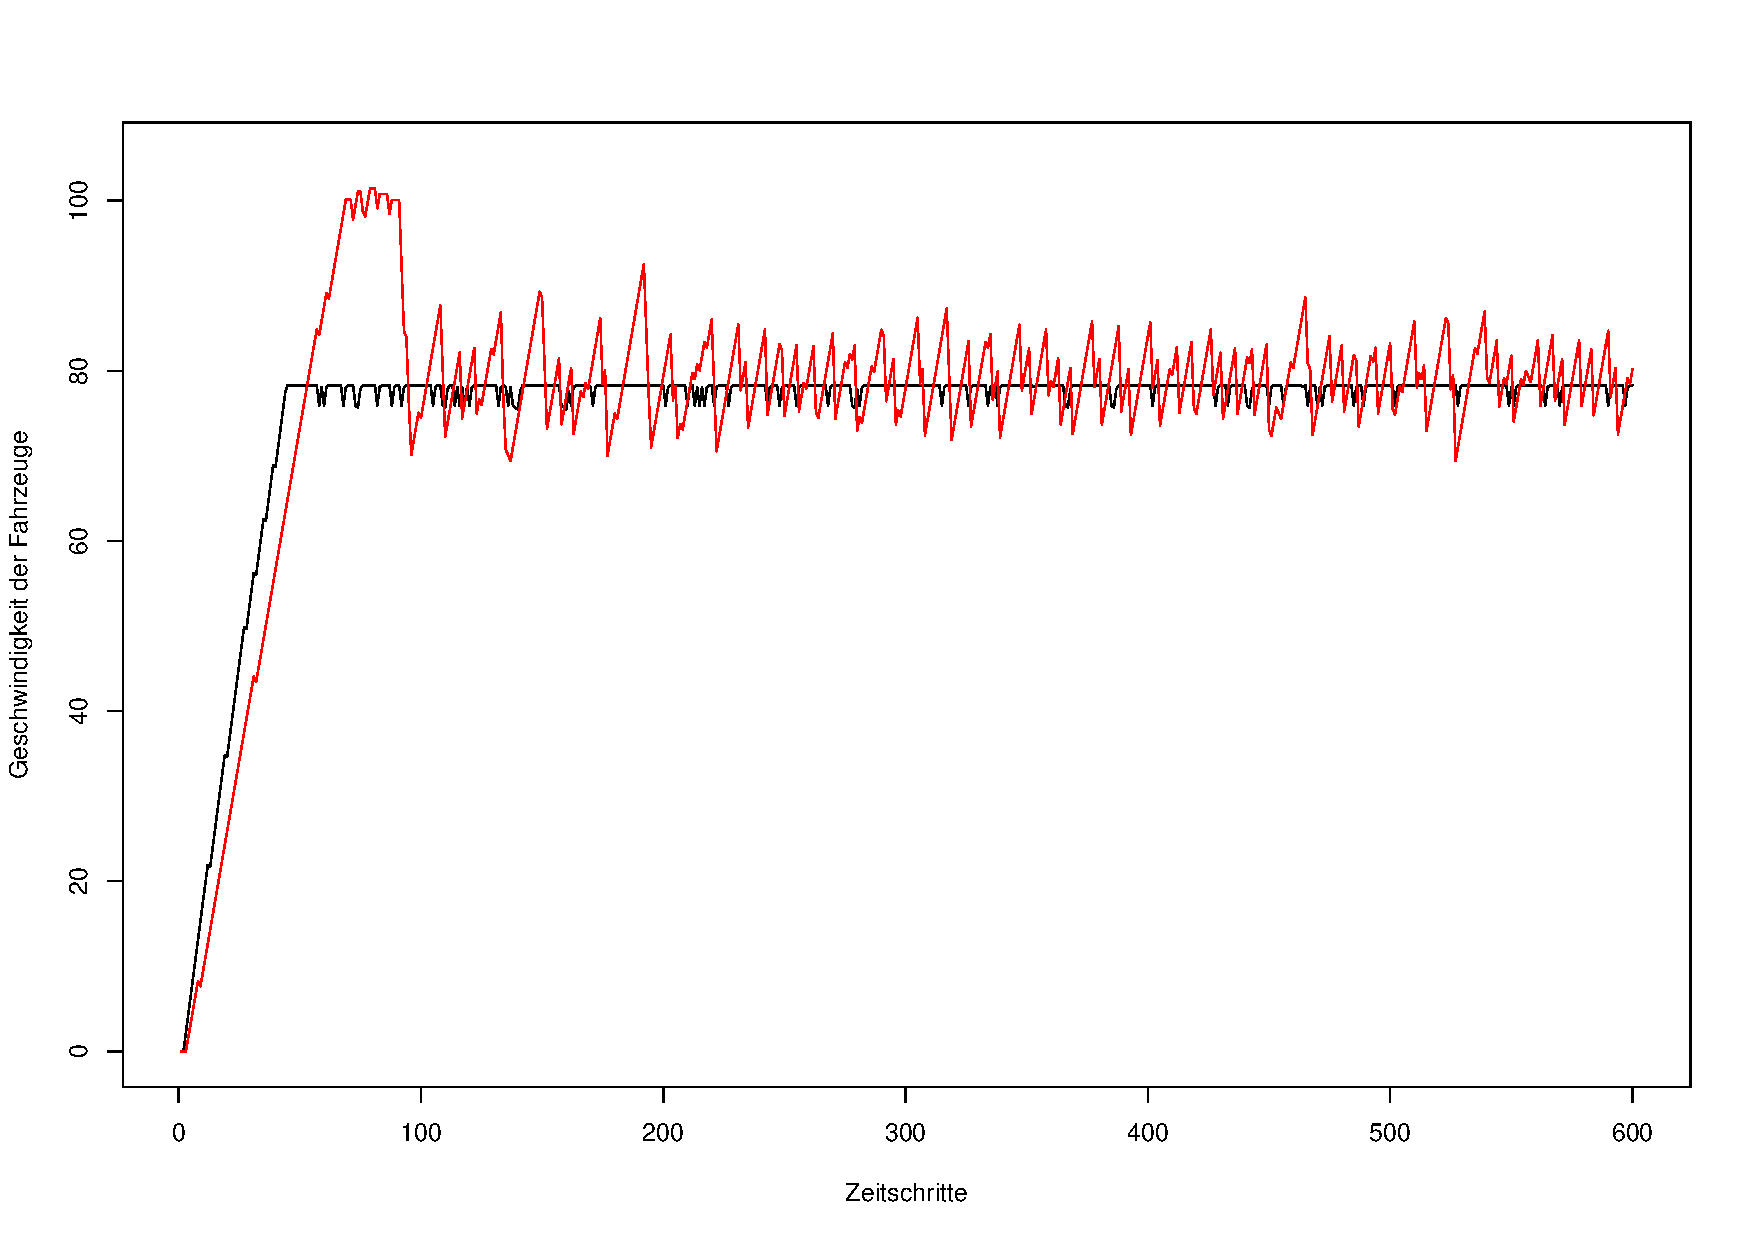
\includegraphics[width=0.3\textwidth]{speed_run25}\label{figure:run25}}\qquad 
   \subfigure[3. Durchlauf]{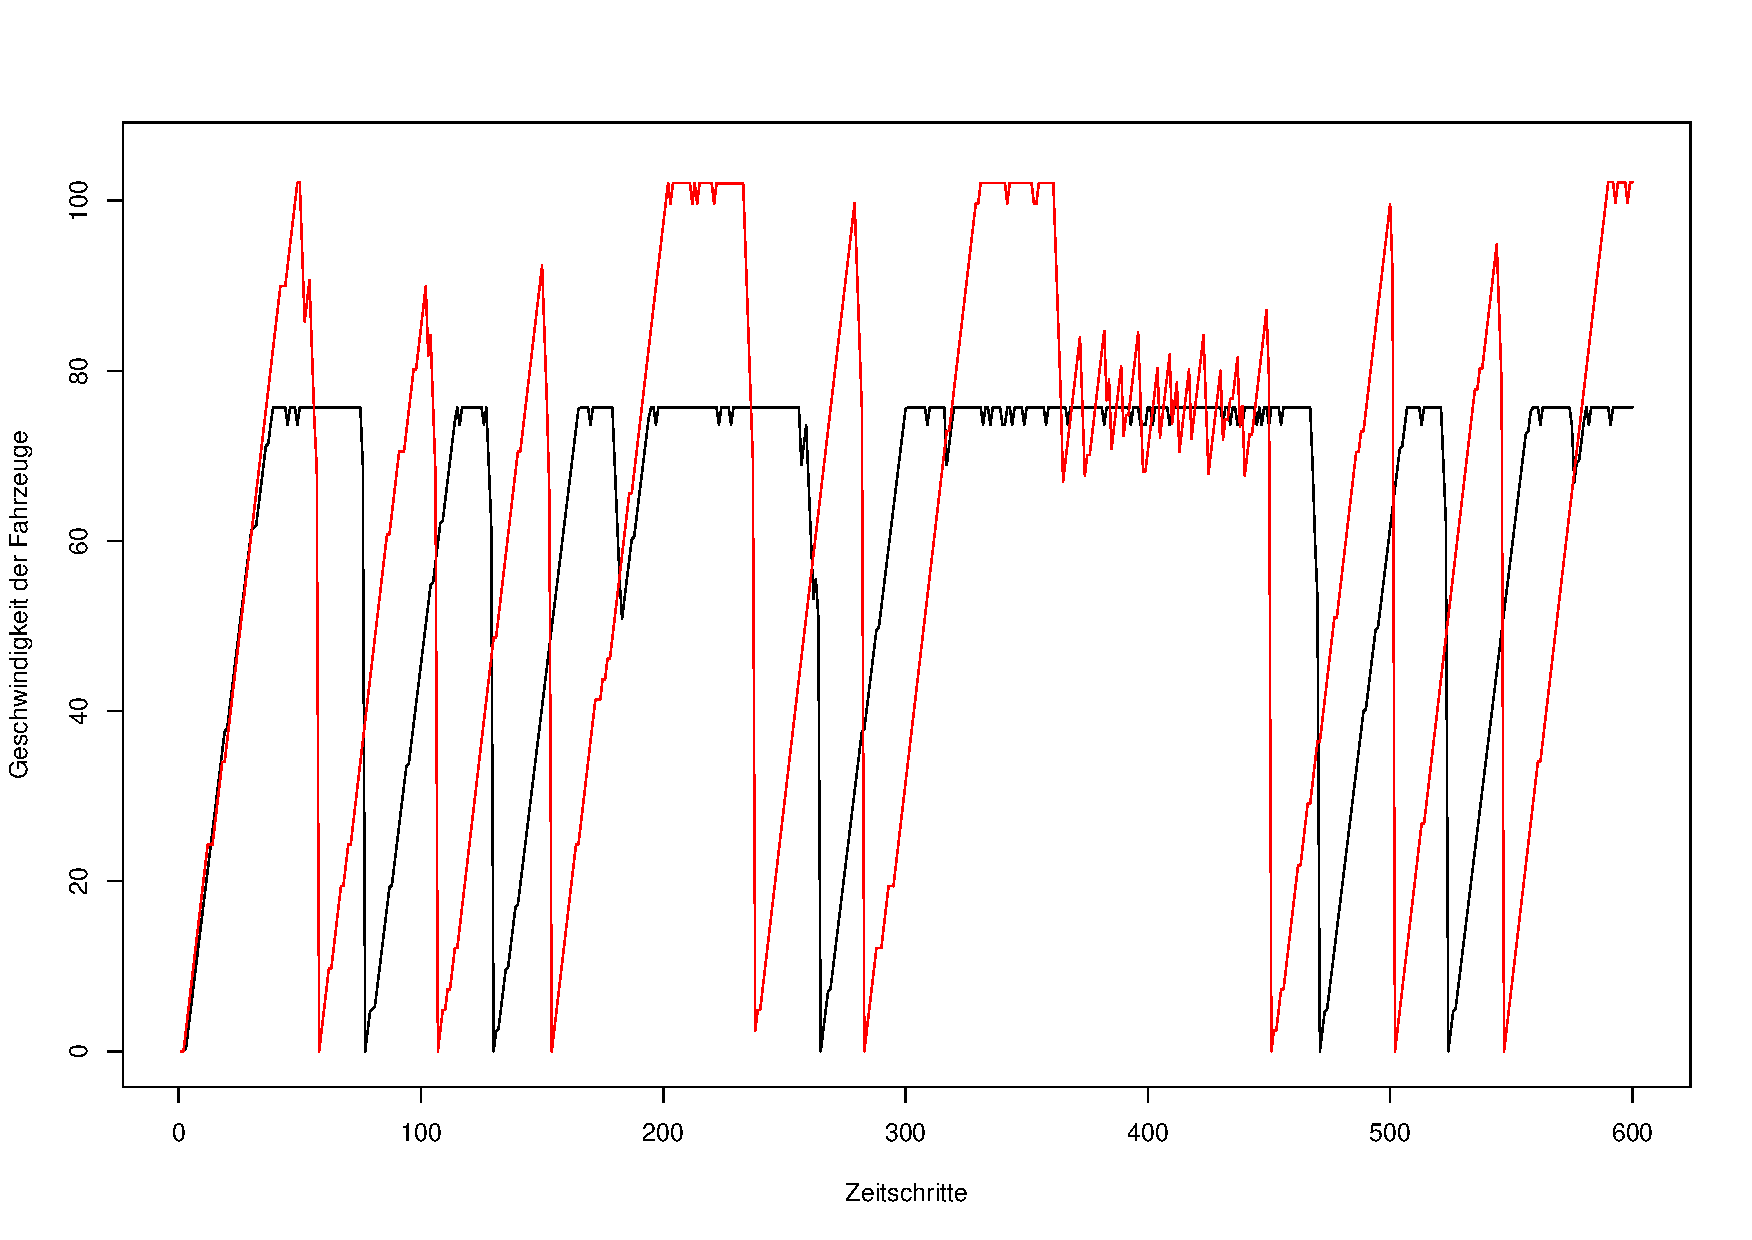
\includegraphics[width=0.3\textwidth]{speed_run26}\label{figure:run26}}
  \caption{Simulationen mit Zellgröße 2,5 m und Zeitschrittlänge 0,05 min} 
  \label{figure:run24-26}
\end{figure}

Die ersten beiden Simulationen mit 2,5 m/0,05 min zeigten ein Bild, welches nach den Veränderungen zu erwarten war.
In der dritten Durchführung traten allerdings wieder Kollisionsereignisse auf.

\begin{figure}[hptb]
  \centering 
   \subfigure[1. Durchlauf]{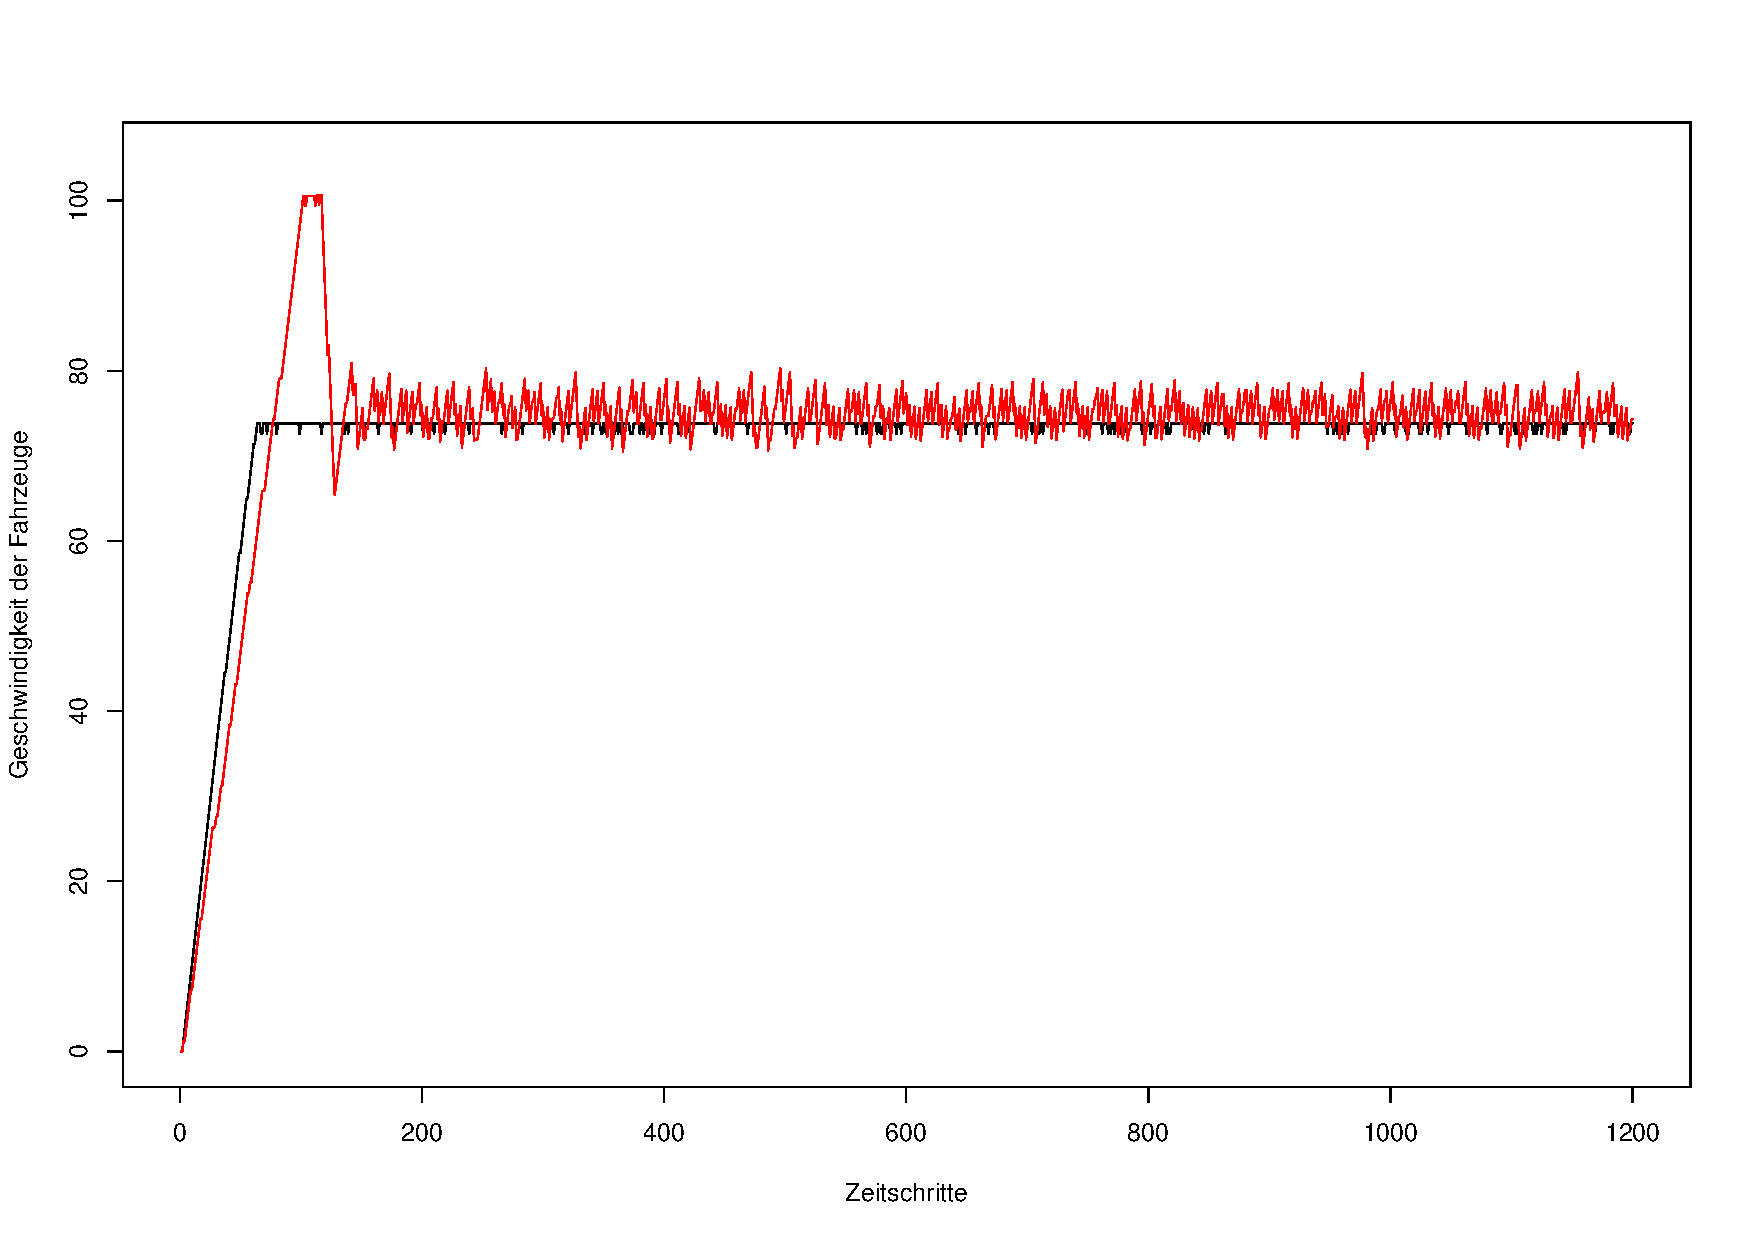
\includegraphics[width=0.3\textwidth]{speed_run27}\label{figure:run27}}\qquad 
   \subfigure[2. Durchlauf]{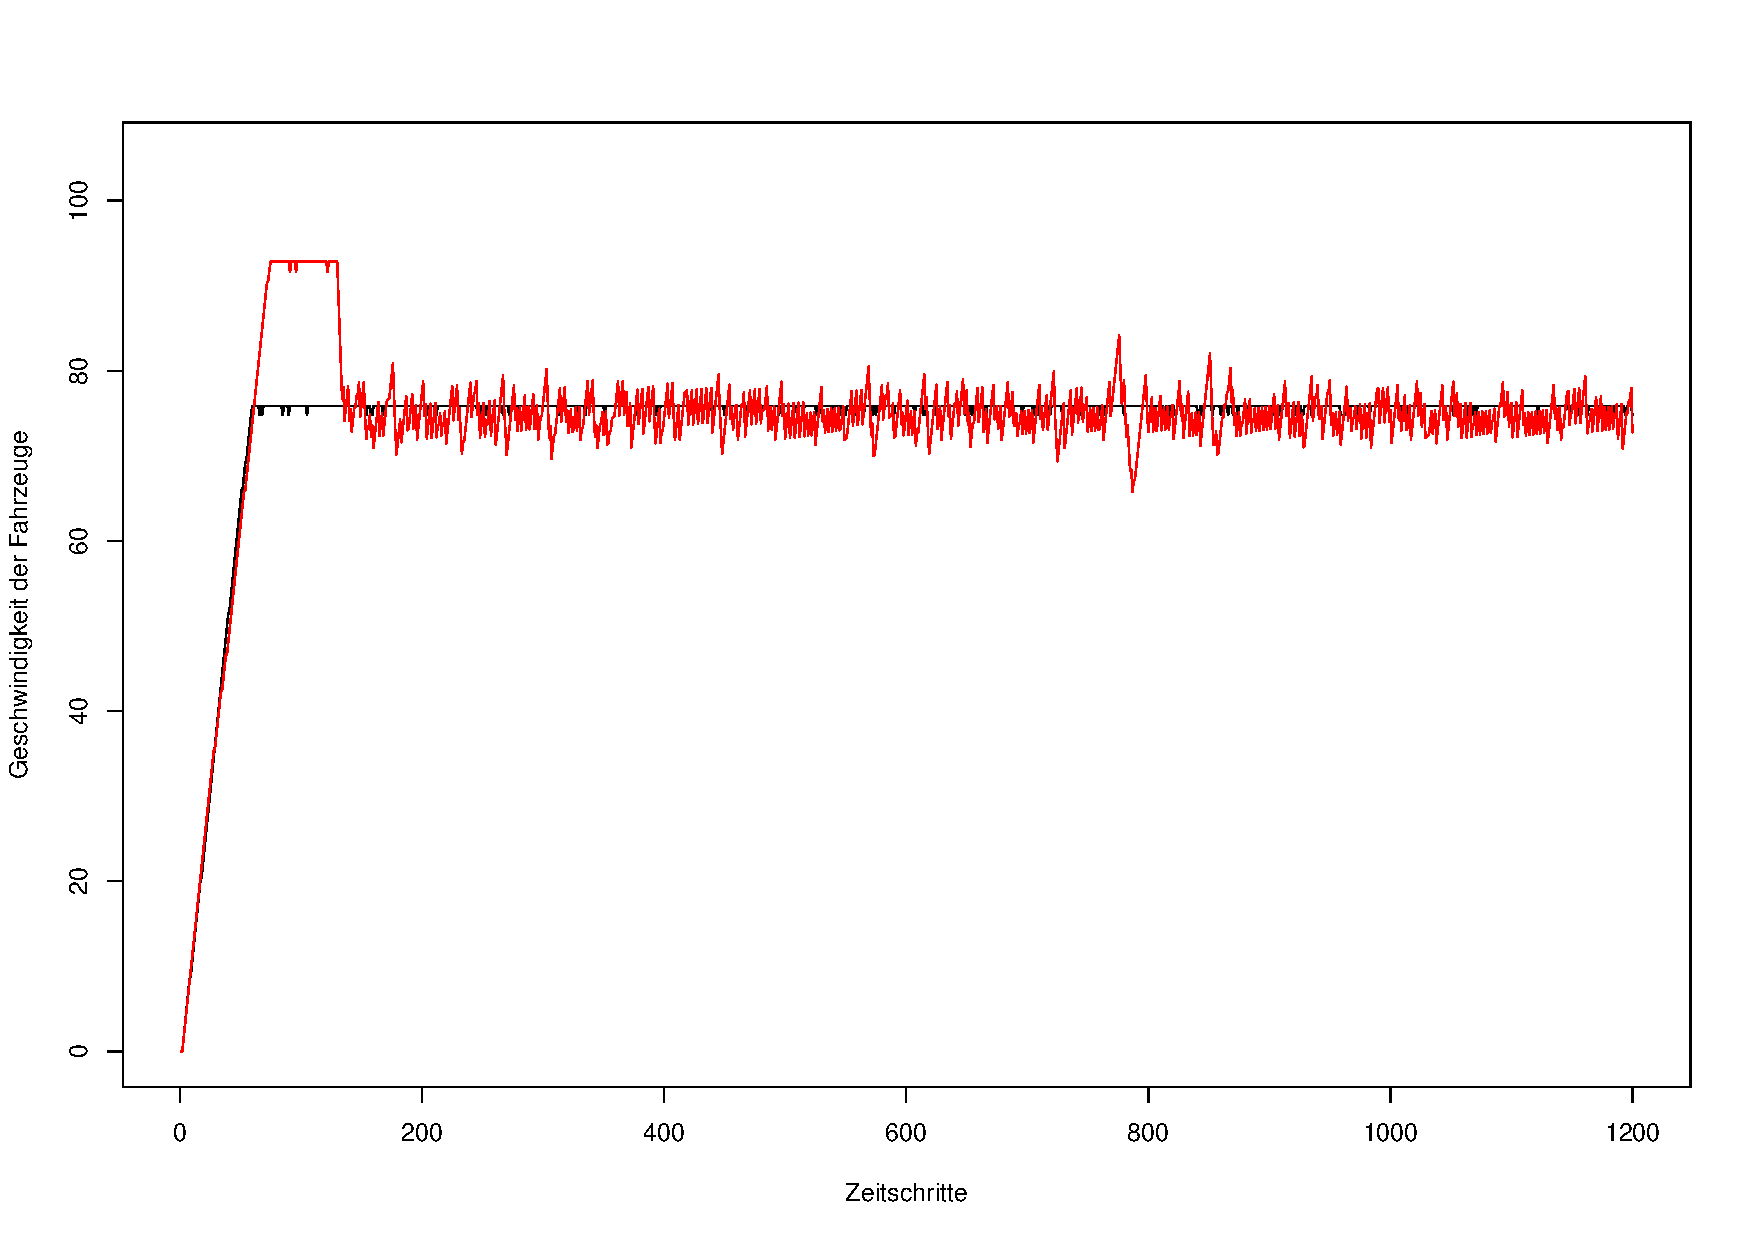
\includegraphics[width=0.3\textwidth]{speed_run28}\label{figure:run28}}\qquad 
   \subfigure[3. Durchlauf]{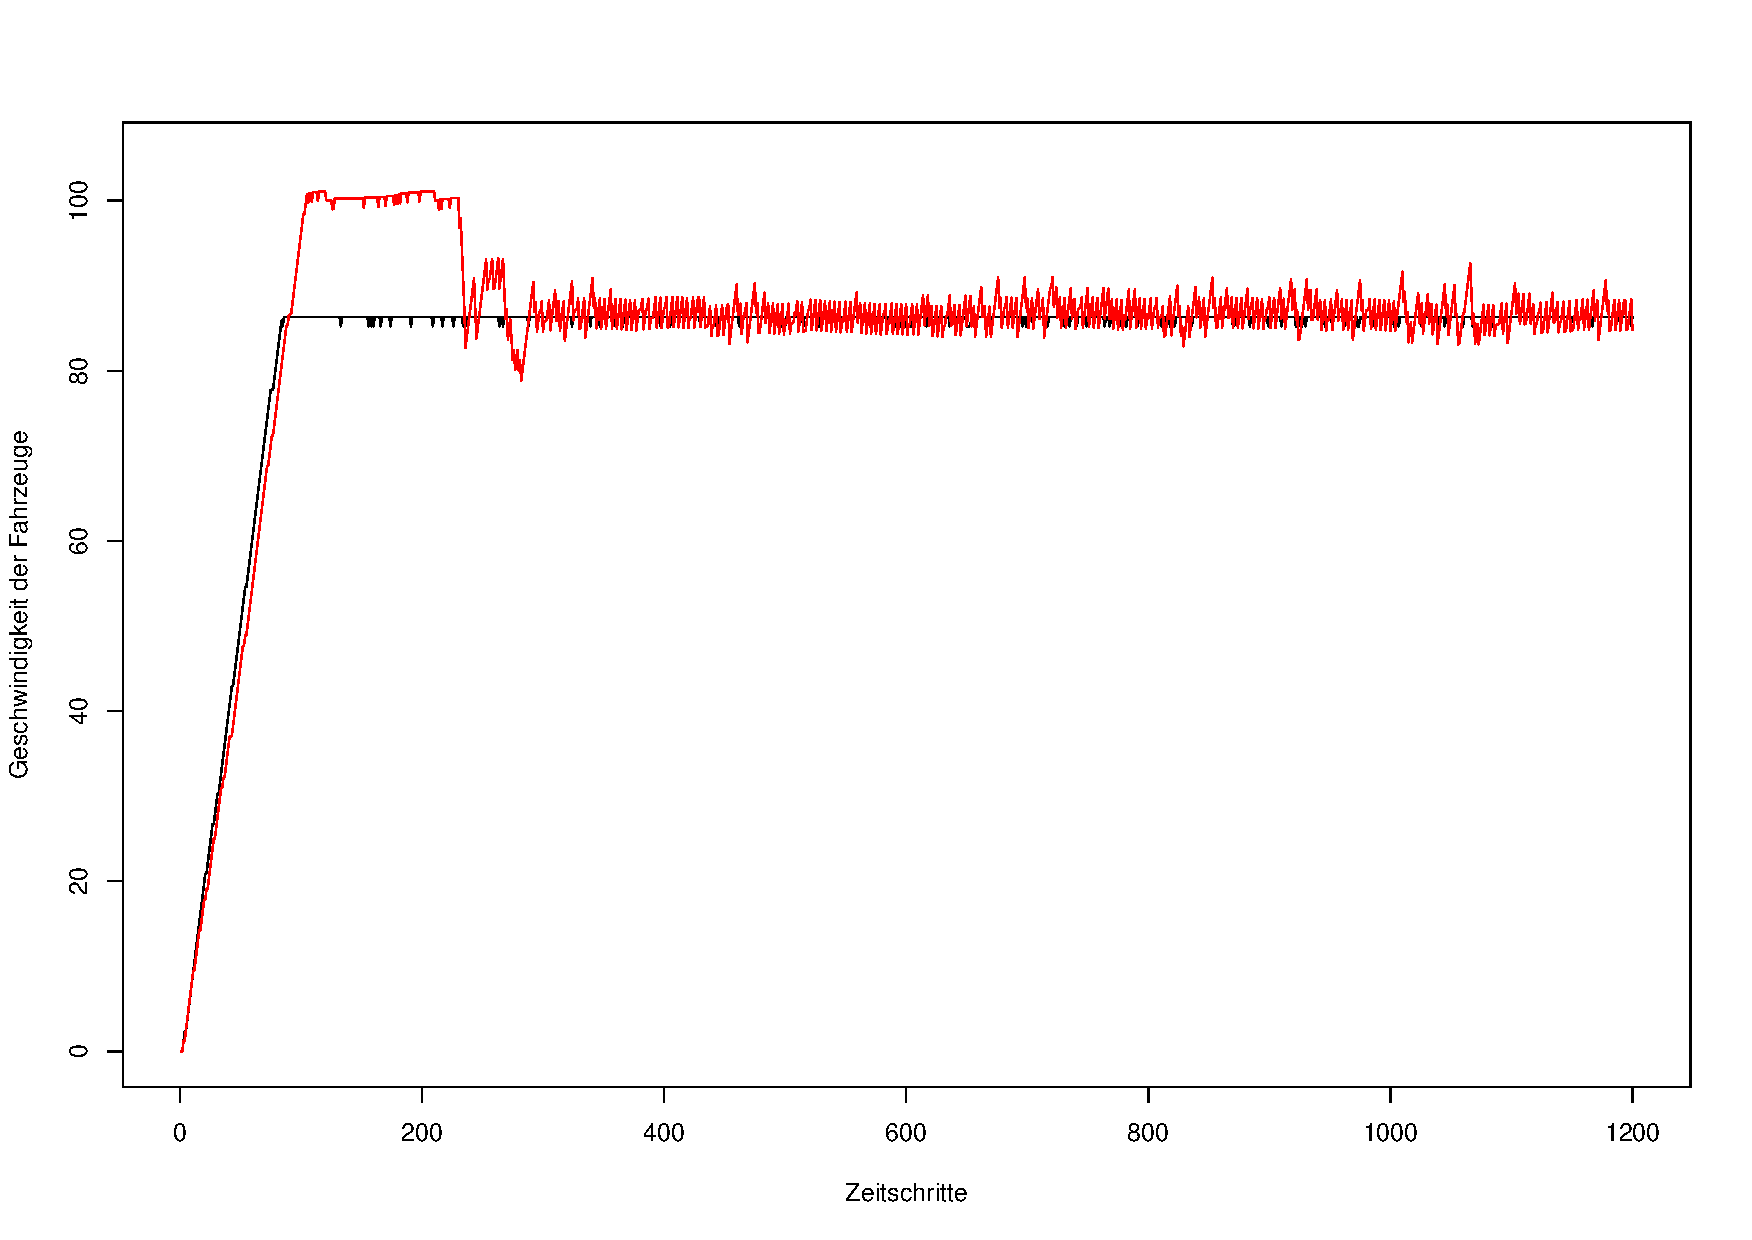
\includegraphics[width=0.3\textwidth]{speed_run29}\label{figure:run29}}
  \caption{Simulationen mit Zellgröße 2,5 m und Zeitschrittlänge 0,025 min} 
  \label{figure:run27-29}
\end{figure}

Die Simulationen der 2,5 m/0,025 min-Variante zeigten [ein sehr gutes Verhalten]\sa{own: anders}.
$Fzg^{S}$ konnte ohne Kollision hinter $Fzg^{L}$ abbremsen und sich dessen Geschwindigkeit anpassen.
\\
Es wurden insgesamt zehn weitere Durchgänge mit diesem Setup durchgeführt. 
Dabei wurde zweimal je eine Kollision beobachtet, die aber immer im Bereich der Beschleunigungsphase am Anfang der Simulation stattfand. 

\subsubsection{\texorpdfstring{Zellgröße $ < $ 2,5 m}%
                              {Zellgröße kleiner als 2,5 m}}

Bei vorhergehenden Testläufen wurde festgestellt, dass es bei einer Zellgröße von weniger als 2,5 Meter zu Inkonsistenzen in den Beliefbases der Agenten kommt.
Entscheidungen müssten dann aufgrund unterschiedlicher Voraussetzungen getroffen werden.
Aus diesem Grund wurde auf den Einsatz von kleineren Zellgrößen verzichtet.





\subsection{Testläufe des Einspurszenarios}
\label{test-singlelane}

Die Testläufe für den Einspurfall erfolgten mit folgenden Einstellungen:
\begin{itemize}
	\itemsep0em
	\item Anzahl Fahrzeuge: variabel
	\item Anzahl Fahrspuren: 1
	\item Streckenlänge: 7,5 km 
	\item Zellgröße: 2,5 m
	\item Simulationsdauer: 2 h
	\item Zeitschrittlänge: 0,025 min (1,5 sek)
	\item Intervalle Beschleunigung/Verzögerung/Geschwindigkeit: $ [3,5; 7] $/$ [8; 10] $/$ [80; 130] $
	\item max. Geschwindigkeit: 100 km/h
	\item Verhalten bei Kollisionsereignis: abbremsen (kein Totalstop)
\end{itemize}

Während bei der Entwicklung durchaus rückwärts laufenden Stauwellen beobachtet werden konnten, ist die Phase der Totalstopps, die dieses Verhalten hervorruft, bei der Simulation im allgemeinen nicht vorhanden.
Durch die feinere Ausführung der Bremsmanöver nähern nähern sich die Positionen der Fahrzeuge einander an und fächern sich, nachdem die Ursache (langsames Fahrzeug) beseitigt ist, wieder auf.














\subsection{Zellgröße vs. Simulation realer Beschleuningung/Verzögerung}

\subsubsection{träges Anfahren}
\label{sec:accelerategroove}

Aufgrund der vergleichbar zum NaSch-Modell gewählten Zellgröße von 7,5 Metern, im Gegensatz dazu aber die Simulation realitätsnaher Beschleunigungswerte, kommt es am Beginn des Simulationslaufs mehrere Zeitschritte lang zu einem Stillstand der Fahrzeuge.
Da jedes Fahrzeug softwareseitig in der Mitte der belegten Zelle platziert wird (bzw. im ersten Zeitschritt dorthin gesetzt wird) wird eine Geschwindigkeit von mehr als $ \frac{1}{2} \times $ 7,5 $ \frac{m}{s} = $ 13,5 km/h benötigt, um eine sichtbare Bewegung durchzuführen.
Durch die unterschiedliche Ausprägung der Beschleunigungswerte ist keine Nennung eines festen Zeitpunkts möglich, an dem dies vollzogen wird.

Im weiteren Verlauf der Simulation fällt es in der Weg-Zeit-Kurve nicht weiter auf, dass die Fahrzeuge an Zellen mit einer bestimmten Länge gebunden sind.



\subsubsection{schlechte Bremswirkung}
\label{sec:bremsverhalten}

Die Simulationsplattform bietet durch realistisch modellierte Beschleunigungen und Verzögerungen den Vorteil, dass der Verkehr feingranularer abgebildet werden kann.
Die analog zu den Simulationen von Nagel und Schreckenberg gewählte Zellgröße von 7,5 Metern führt allerdings dazu, dass theoretisch dargestellte Reduktionen der Geschwindigkeit nicht direkt in nächsten Zeitschritt umgesetzt werden.
Vielmehr muss, ähnlich wie beim Losfahren, siehe \cref{sec:accelerategroove}, ein gewisser Wert unterschritten werden, damit die gezeigte Bewegung auch real kürzer gesetzt wird.

Reicht der Platz nach vorn nicht aus, um das Fahrzeug entsprechend seiner Geschwindigkeit zu bewegen und in die freie Zelle hinter das vorausfahrende Fahrzeug zu setzen, wird ein Kollisionsereignis ausgelöst.

Das Verhalten hierzu kann über den Agentenplan gesteuert werden.
Zu Beginn der Erarbeitung wurde die Kollision mit einem extremen abbremsen modelliert, später dann als Totalstopp.
\\
Die Reduktion der Geschwindigkeit auf Null ist insofern vorteilhaft, weil der Extremausschlag nach unten im Plot der Geschwindigkeiten sichtbar ist.
Außerdem wird der Agent wirklich in der aktuellen Zelle gestoppt. 
Die Simulationsplattform würde sonst über (mehrere) Zeitschritte hinweg die Geschwindigkeit abzubauen, ohne dass bedingt durch vorausliegende Hindernisse, eine reale Bewegung stattfinden könnte. 
\\
Nachteilig ist zu sehen, dass ein Totalstillstand aufgrund der großen Geschwindigkeitsunterschiede meist weitere Kollisionen nach sich zieht.

% --- Diese beiden Absätze sind gut - Phil FB 27feb
Die Schwierigkeiten beim Bremsen können durch Reduktion der Zellgröße bei ansonsten gleichen Voraussetzungen \enquote{behoben} werden.
Eine Simulation mit reduzierten Zellgrößen führte in diesem Aspekt zu einem harmonischeren Verkehrsbild.

Für die weitere Entwicklung könnte für die Fahrzeuge bei der Initialisierung eine Länge generiert werden, wodurch diese mehrere dieser dann kleineren Zellen überdecken würden.
Dies würde ein diversifizierteres Fahrzeugbild zur Folge haben, bzw. die Möglichkeit eröffnen präzisere Simulationen mit kleineren Zellen durchzuführen und Fahrzeugklassen auch in Sachen Platzbedarf realistisch erscheinen zu lassen.


\subparagraph*{Worst Case-Analyse für Mindestabstände}

Das Kollisionsereignis wird nicht erst bei einer tatsächlichen Kollision, also wenn sich zwei Fahrzeuge in einem Punkt treffen, ausgelöst, sondern bereits wenn der Platz nach vorn zum aktuellen Zeitpunkt nicht mehr zum bewegen ausreicht.
Hierbei spielt es für das Simulationstool keine Rolle, dass das Hindernis in Bewegung ist und sich von dort entfernt.

In \cref{tab:restgeschw-abstand} sind die Mindestabstände für eine kollisionsfreie Bewegung für eine Zellgröße vom 2,5 m und einer Zeitschrittgröße von 0,025 min aufgeführt.
Zwischenschritte der Berechnung wurden jeweils aufgerundet.

\begin{table}[ht]
\begin{center}
\setlength{\tabcolsep}{0.5em} % for the horizontal padding
{\renewcommand{\arraystretch}{1.2}% for the vertical padding
\begin{tabular}{| c  c  c |}
\hline 
Restgeschwindigkeit & Mindestabstand in m \\ \hline 
130 & 55 \\ 
100 & 43 \\ 
80 & 35 \\ 
70 & 30 \\ 
60 & 25 \\ 
50 & 23 \\ 
30 & 13 \\ 
Schritt & 3 \\ \hline
\end{tabular}
}
\caption{Mindestabstände für Restgeschwindigkeit}
\label{tab:restgeschw-abstand}
\end{center}
\end{table}

Eine Veränderung der Zellgröße verändert diese Werte nicht grundlegend. 
Es wird meist lediglich auf ein Vielfaches der Zellgröße gerundet.
\\













%%.\sa{hier vermischst Du \cref{sec:sota} mit \cref{sec:realisierung}, hier geht es darum, wi Du konkret arbeiten willst um die Sachen unter \cref{sec:researchgap} zu beweisen oder zu belegen, evtl macht es Sinn diese Punkte mit in \cref{sec:sota} zu ziehen, Du kannst dann einfach, wenn Du es brauchst Verweise setzen}
%
%\noindent
%Die in \cite{dat-ba} vorgeschlagene Struktur ist zu implementieren und in vergleichbarer Umgebung simulatorisch zu testen. 
%Dabei sind die folgenden Größen zu erheben und entsprechend statistisch auszuwerten: 
%
%\begin{itemize}
%\item Verkehrsdichte
%\item Verkehrsfluss
%\item Spurwechselfrequenz
%\item Spurnutzung links/rechts
%\end{itemize}
%
%Das Testszenario wurde in \cite{na-sch} durch das zu Beginn zufällige Platzieren von Fahrzeugen in einem geschlossenen Kreis mit $L$ Zellen (ähnlich einer Autorennstrecke) simuliert. \\
%Allerdings wurde auch, bei der Simulation einer Fahrbahnverengung, eine Alternative Simulationsmöglichkeit beschrieben. 
%Eine Gridgerade von bis zu 10000 Zellen Länge wurde getestet - Bewegungsrichtung von links nach rechts. 
%Die Fahrzeuge wurden mit $v=0$ in die am weitesten links befindliche Zelle, so diese frei war, gesetzt und die Fahrzeuge in den sechs am weitesten rechts befindlichen Zellen (bei systemweiter $v_{max}=5$) gelöscht. 
%Letzteres Vorgehen sorgte für eine offene Grenze für den abfließenden Verkehr.
%
%Für eine kontinuierliche Simulation ist die zweite Möglichkeit ungeeignet. 
%Auch in \cite{multi-lane} wird von der Nutzung periodischer Randbedingungen gesprochen. 
%Dies lässt darauf schließen, dass, wie in \cite[Abb. 1.5]{peri-rand} für die Umgebung von Pixeln beschrieben, die Fahrzeuge vom \enquote*{Ende} der Gridstrecke am \enquote*{Anfang} wieder eingesetzt wurden und somit der zuerst beschriebene Kreis einsteht.
%Dieses Verhalten ist zu bevorzugen.
%
%Vorteil der geschlossenen Kreisstrecke ist, dass man bei konstanter Fahrzeuganzahl $N$ (bei \cite{multi-lane} waren dies $N = 10^{3}$) durch die Veränderung der Systemgröße eine unterschiedliche Fahrzeugdichte erreicht werden kann. 
%Jeder Dichtewert wurde für $T = 10^{5}$ Zeitschritte simuliert, wobei die erste Hälfte verworfen wurde, um mögliche Störeffekte ausklingen zu lassen. 
%Die generierten Simulationsdaten wurden über $T_{sample} = 300$ Zeitschritte und eine Wegstrecke von 133 Zellen, was etwa 1 km Länge in der realen Welt entspricht, gemittelt, um statistische Schwankungen zu reduzieren.
%
%Ein mögliches Simulationstool ist das \enquote{Traffic Simulation Game}\footnote{\link{https://lightjason.github.io/news/2017-09-workshop/}}. 
%In der Grundkonfiguration erzeugt dieses eine beliebig lange, gerade Straße mit beliebig vielen Fahrspuren. 
%ſEs ist zu prüfen, ob die Software auf die gewünschte Verhaltensweise angepasst werden kann.
    
    \bibliography{references}

\end{document}

